% Ejemplo de documento de tesis.
% Versión:
% $Id: main.tex 647 2009-06-25 20:08:54Z lm-mac $
%
% Una tesis en inglés y de la UC3M sería:
\documentclass[11pt,spanish,UC3MThesis]{PhdThesis}
%
% Una tesis en español y de la UH sería:
%\documentclass[11pt,spanish,UHThesis]{PhdThesis}
\usepackage{babel,tabularx,ctable}
\usepackage{algorithmic}
\usepackage{pdfpages}
%----------------------------------------
% opciones para hyperref
% enlaces en colores, convenientes para visualizar el documento.
\newcommand\MYhyperrefoptions{bookmarks=true,bookmarksnumbered=true, pdfpagemode={UseOutlines},plainpages=false,pdfpagelabels=true,
colorlinks=true,linkcolor={blue},citecolor={blue},pagecolor={blue}, urlcolor={blue}, 
pdftitle={Programacion Genetica Aplicada a la Resolucion del Cubo de Rubik}, 
pdfsubject={Proyecto de Fín de Carrera},
pdfauthor={Ignacio Bona Piedrabuena},
pdfkeywords={}}
% enlaces en blanco y negro, mejor para la versión final
%newcommand\MYhyperrefoptions{bookmarks=true,bookmarksnumbered=true,pdfpagemode={UseOutlines},
%plainpages=true,pdfpagelabels=true,colorlinks=true,linkcolor={black},citecolor={black},pagecolor={black}, urlcolor={black},
%pdftitle={Understanding New Orleans}, 
%pdfsubject={Another PhD Thesis},
%pdfauthor={Ignatius O'Reilly},
%pdfkeywords={katrina,new orleans,jeans}}
%
% incluyendo hyperref
\usepackage[\MYhyperrefoptions,pdftex]{hyperref} % para pdflatex
%\usepackage[hypertex, colorlinks=true, backref]{hyperref} % para latex
%----------------------------------------
%
% otros paquetes
\usepackage[utf8]{inputenc}
\usepackage[caption=false,font=footnotesize]{subfig}
\usepackage{graphicx}
%
%  declarando estilo de bibliografía
\usepackage[round,sort&compress]{natbib}
% redefiniendo \cite para que apunte a la cita más común de natbib
\renewcommand{\cite}[1]{\citep{#1}}
%
% cambiar tipo de letras
%\usepackage[charter]{mathdesign}
%\usepackage[math]{iwona}
\usepackage{cmbright}
\usepackage[cmbright]{sfmath}

% para las tablas
\renewcommand{\tabularxcolumn}[1]{>{\centering\arraybackslash}m{#1}}
\setlength{\heavyrulewidth}{0.1em}
\newcommand{\otoprule}{\midrule[\heavyrulewidth]}

%
%---------------------------------------
% 
\title{Programación Genética Aplicada a la Resolución del Cubo de Rubik}
\author{Ignacio Bona Piedrabuena}
\supervisor{Luis Martí Orosa}
% usando href estas cosas quedan mejor
%\email{\href{mailto:reilly@uc3m.es}{reilly@uc3m.es}}
%\homepage{\href{http://www.giaa.inf.uc3m.es/miembros/reilly}{http://www.giaa.inf.uc3m.es/miembros/reilly}}
%\address{31415 Katrina St, New Orleans 21780 \\ Lousiana, United States}
%
%\telephone{+34 91 856 13XX}
\date{Colmenarejo, 2010} 
%
% si el documento no es una tesis doctoral lo puedes cambiar aquí
\thesiscustomname{Proyecto de Fín de Carrera}
%
\makeindex
\setlength{\parskip}{1ex plus 0.5ex minus 0.2ex}
\begin{document}
\renewcommand{\tablename}{Tabla} 
%\pagestyle{empty}
\chaptertitlestyle{serifbig}
\partstyle{serifbig}
\pagestyle{serif}

\maketitle
 \begin{dedication}
 	\textit{Para mi copiloto.}
 \end{dedication}
%\begin{abstract}
%    In this work we present 
%\end{abstract}
\begin{acknowledgments}
 	Me gustaría agradecer a todas aquellas personas que me han apoyado no sólo
 	en la realización de este proyecto, sino a todos aquellos que me han ayudado
 	a llegar hasta aquí. A mi madre. A mi padre. A mi hermano. A toda mi familia
 	que me apoya en cada momento. A Azahara y a su familia por hacerme sentir
 	como uno más. A Enrique por terminar el proyecto casi a la vez. A todos
 	aquellos amigos que nos hemos mantenido con fuerzas examen tras
 	examen: Alexis, Dani, Acebes, Lidia, Jorge y muchos más. A Crazy Soul: Abtin,
 	Gonzo, Marc, Joseba. A Against The Odds: Roberto, Edu y Jesús por perseguir
 	un sueño. A todos aquellos amigos y amigas que nos hacer pasar tan buenos
 	momentos: Kim, Isa, Cris, Govi, Erica, Nacho, Alba, Arázazu, Ali. A mis
 	compañeros de beca: Dani, Miguel. A mis viejos amigos: Fer, Pablo, Victor, Diego, Jorge. A mis
compañeros de trabajo: Javier, Marisol, Pepón, Javier Izquierdo, Amaia,
 	Carlos, Guillermo. A mi vecino y amigo de toda la vida Santi. A Luis por su paciencia y apoyo, gracias a los
 	cuales he logrado que este proyecto llegue a buen puerto. A todos
 	aquellos que se me olvide nombrar.
 	
 	Y, en especial, a aquellos que ya no están aquí. A mi abuelo. A Loli.
 	
 	A todos ellos gracias.
\end{acknowledgments}
\frontmatter 
\tableofcontents
%\listoffigures
%\listoftables
%\begin{preface}
%    Here the preface
%\end{preface}
%if you use only (sub)section* in introduction



\mainmatter
%\bibliography{bib/biblio}
\chapter{Introducción}\label{ch:intro}

En este proyecto de fin de carrera se tiene como objetivo tratar el tema de la
programación genética. De esta forma se pretende generar un programa que resuelva
el cubo de Rubik de forma óptima. El motivo del proyecto se debe a una
competición ofrecida por Parabon, en la que se pretende participar. El ganador
de la competición tendrá la oportunidad de exponer su proyecto en \textit{The
Genetic and Evolutionary Computation Conference 2009} (GECCO 2009),
una famosa conferencia sobre la computación evolutiva.

La programación genética es una rama de la computación evolutiva donde se imita
el modelo de evolución natural aplicado a programas informáticos. La computación
evolutiva procede de difqerentes orígenes: programación evolutiva
\cite{Fogel:1966}, algoritmos genéticos \cite{Holland:1975}, estrategias de
evolución \cite{Rechenberg:1971,Schwefel:1975} y por último programación genética
\cite{Cramer:1985,Koza:1992}. Todas estas vertientes nacieron de forma
independiente, pero en los noventa se unificaron para formar la computación
evolutiva.  Todas estas ramas coinciden en inspirarse en la teoría de la
evolución moderna de la que Darwin \cite{Darwin:1859} plantó sus pilares, para
resolver problemas, normalmente de optimización, en la informática.

La computación evolutiva se caracteriza por encontrar soluciones inusuales a
problemas de los que no existe un método resolutivo claro o viable en términos
temporales. La potencia de estos sistemas reside en una multitudinaria
exploración aleatoria del espacio búsqueda.

Uno de los problemas del cubo de Rubik es que debido al gran número de
posibilidades de desorden no es posible determinar a priori un número mínimo de
pasos que se necesitan para resolver cualquier cubo. De este modo, los métodos
que han dado mejores resultados han sido los sistemas de búsquedas exhaustivas
informáticas,  batiendo el record con 26 pasos \cite{Cooperman-Kunkle:2007} y
22 pasos \cite{Rokicki:2008}. Sin embargo, explorar todo el extenso espacio de
cubos de Rubik posibles resulta un proceso muy costoso, por lo que es posible que
aún existan soluciones más cortas inexploradas actualmente. Esto hace que la
programación genética sea un desafío interesante para la resolución mediante la
computación evolutiva.

El resto de este documento trendrá la siguiente estructura. Un capítulo
introductorio donde se describirá de la teoría de la evolución en la que se
inspiran las principales ideas de los sistemas evolutivos
(capítulo \ref{ch:estado-arte}). Procederemos a adentrarnos en la  situación actual de los sistemas evolutivos, en concreto en la programación evolutiva, donde se verán todos los procesos existentes en una evolución informática. Además profundizaremos y
describiremos los métodos más utilizados en la programación evolutiva, con sus
ventajas y sus defectos.

Una vez introducidos en la materia de la programación genética fijaremos los
objetivos de este proyecto de fin de carrera (capítulo \ref{ch:objetivos}).

\begin{itemize}
  \item Desarrollo de una representación adecuada del problema para hacer posible su solución usando
  programación genética.
  \item Experimentación y ajuste de los parámetros del algoritmo evolutivo a fin de lograr soluciones con el
  mejor desempeño posible.
  \item Ejecución del sistema y extracción de la mejor solución para ser
  enviada a la competición.
\end{itemize}

En el capítulo \ref{ch:diseno-algoritmo} explicaremos el diseño de nuestro algoritmo que hemos
utilizado para la realización de este proyecto. Veremos las evoluciones que ha
sufrido nuestro lenguaje hasta llegar hasta el seleccionado para ser
implementado. Además hablaremos de todo el complejo proceso de evaluación y
asignación del fitness a nuestros individuos.

Una vez abordado el diseño del sistema, nos centraremos en la implementación
(capítulo \ref{ch:implementacion}). Explicaremos las herramientas que nos han
ayudado a desarrollar un programa evolutivo, además de las librerías que modelan
el cubo de Rubik computacionalmente. Terminaremos este capítulo explicando la
implementación con diagramas de clases y la configuración final de la
plataforma evolutiva.

En el capítulo \ref{ch:pruebasyresultados} hablaremos de las pruebas realizadas, explicando el
porqué de ellas y las conclusiones de su resultado.

Las conclusiones finales del proyecto se verán en el capitulo \ref{ch:concl}, además de
hablar de las futuras líneas de investigación.

Como anexos añadiremos la planificación del proyecto y un desarrollo en detalle
de los parámetros de utilización de ECJ.

% otherwise use
% \mainmatter
% %\bibliography{bib/biblio}
\chapter{Introducción}\label{ch:intro}

En este proyecto de fin de carrera se tiene como objetivo tratar el tema de la
programación genética. De esta forma se pretende generar un programa que resuelva
el cubo de Rubik de forma óptima. El motivo del proyecto se debe a una
competición ofrecida por Parabon, en la que se pretende participar. El ganador
de la competición tendrá la oportunidad de exponer su proyecto en \textit{The
Genetic and Evolutionary Computation Conference 2009} (GECCO 2009),
una famosa conferencia sobre la computación evolutiva.

La programación genética es una rama de la computación evolutiva donde se imita
el modelo de evolución natural aplicado a programas informáticos. La computación
evolutiva procede de difqerentes orígenes: programación evolutiva
\cite{Fogel:1966}, algoritmos genéticos \cite{Holland:1975}, estrategias de
evolución \cite{Rechenberg:1971,Schwefel:1975} y por último programación genética
\cite{Cramer:1985,Koza:1992}. Todas estas vertientes nacieron de forma
independiente, pero en los noventa se unificaron para formar la computación
evolutiva.  Todas estas ramas coinciden en inspirarse en la teoría de la
evolución moderna de la que Darwin \cite{Darwin:1859} plantó sus pilares, para
resolver problemas, normalmente de optimización, en la informática.

La computación evolutiva se caracteriza por encontrar soluciones inusuales a
problemas de los que no existe un método resolutivo claro o viable en términos
temporales. La potencia de estos sistemas reside en una multitudinaria
exploración aleatoria del espacio búsqueda.

Uno de los problemas del cubo de Rubik es que debido al gran número de
posibilidades de desorden no es posible determinar a priori un número mínimo de
pasos que se necesitan para resolver cualquier cubo. De este modo, los métodos
que han dado mejores resultados han sido los sistemas de búsquedas exhaustivas
informáticas,  batiendo el record con 26 pasos \cite{Cooperman-Kunkle:2007} y
22 pasos \cite{Rokicki:2008}. Sin embargo, explorar todo el extenso espacio de
cubos de Rubik posibles resulta un proceso muy costoso, por lo que es posible que
aún existan soluciones más cortas inexploradas actualmente. Esto hace que la
programación genética sea un desafío interesante para la resolución mediante la
computación evolutiva.

El resto de este documento trendrá la siguiente estructura. Un capítulo
introductorio donde se describirá de la teoría de la evolución en la que se
inspiran las principales ideas de los sistemas evolutivos
(capítulo \ref{ch:estado-arte}). Procederemos a adentrarnos en la  situación actual de los sistemas evolutivos, en concreto en la programación evolutiva, donde se verán todos los procesos existentes en una evolución informática. Además profundizaremos y
describiremos los métodos más utilizados en la programación evolutiva, con sus
ventajas y sus defectos.

Una vez introducidos en la materia de la programación genética fijaremos los
objetivos de este proyecto de fin de carrera (capítulo \ref{ch:objetivos}).

\begin{itemize}
  \item Desarrollo de una representación adecuada del problema para hacer posible su solución usando
  programación genética.
  \item Experimentación y ajuste de los parámetros del algoritmo evolutivo a fin de lograr soluciones con el
  mejor desempeño posible.
  \item Ejecución del sistema y extracción de la mejor solución para ser
  enviada a la competición.
\end{itemize}

En el capítulo \ref{ch:diseno-algoritmo} explicaremos el diseño de nuestro algoritmo que hemos
utilizado para la realización de este proyecto. Veremos las evoluciones que ha
sufrido nuestro lenguaje hasta llegar hasta el seleccionado para ser
implementado. Además hablaremos de todo el complejo proceso de evaluación y
asignación del fitness a nuestros individuos.

Una vez abordado el diseño del sistema, nos centraremos en la implementación
(capítulo \ref{ch:implementacion}). Explicaremos las herramientas que nos han
ayudado a desarrollar un programa evolutivo, además de las librerías que modelan
el cubo de Rubik computacionalmente. Terminaremos este capítulo explicando la
implementación con diagramas de clases y la configuración final de la
plataforma evolutiva.

En el capítulo \ref{ch:pruebasyresultados} hablaremos de las pruebas realizadas, explicando el
porqué de ellas y las conclusiones de su resultado.

Las conclusiones finales del proyecto se verán en el capitulo \ref{ch:concl}, además de
hablar de las futuras líneas de investigación.

Como anexos añadiremos la planificación del proyecto y un desarrollo en detalle
de los parámetros de utilización de ECJ.

% with \chapter{\introductionname} instead of \introduction

\chapter{Estado del arte}\label{ch:estado-arte}

\section{Teoría de la evolución}

La computación evolutiva está basada, como muchos otros saberes humanos, en la
observación y funcionamiento de la naturaleza. Como la propia palabra anticipa,
la computación evolutiva imita al proceso de evolución natural para alcanzar
objetivos computacionales. Esta descripción es una breve explicación de ciertos
fenómenos naturales que nos servirán para entender mejor la computación
evolutiva.

¿Qué es el código genético?  El código genético es el conjunto de normas por las que la información codificada
en el material genético (secuencias de ADN o ARN) se traduce en proteínas (secuencias de aminoácidos) en las
células vivas. Esto significa que el código genético almacena toda la información física de nuestro cuerpo:
color de la piel, color de ojos, altura de las orejas, etc. No obstante, la información aprendida durante la
vida no se almacena en los genes (código genético). De esta forma, nuestros hijos se parecen a nosotros porque
llevan parte de nuestro código genético, sin embargo, no actúan de la misma manera, ya que el comportamiento
depende de muchos otros factores (educación, amistades, sociedad). Por ejemplo, los gemelos son idénticos
genéticamente y, por ello, su apariencia externa es la misma; pero su forma de actuar puede ser completamente
diferente.

El código genético está formado por una o varias cadenas de ácido
desoxirribonucleico o ADN. A su vez estas cadenas están formadas por cuatro
nucleótidos cuyas bases son: adenina (A), timina (T), citosina (C) o guanina (G).
Estas bases se unen entre sí formando largas cadenas de información
(AGGTACGTAATTCTGTCG…). Las secuencias de ADN que constituyen la unidad
fundamental, física y funcional de la herencia se denominan genes (figura
\ref{fig:adn}). De esta forma llamaremos gen a la parte de ADN que codifica, por
ejemplo, el color de los ojos. Realmente, toda esta información genética se asemeja a un lenguaje, y como todo
lenguaje, tiene reglas gramaticales y sintácticas, y una posterior interpretación
y expresión.

\begin{figure}[t] \centering
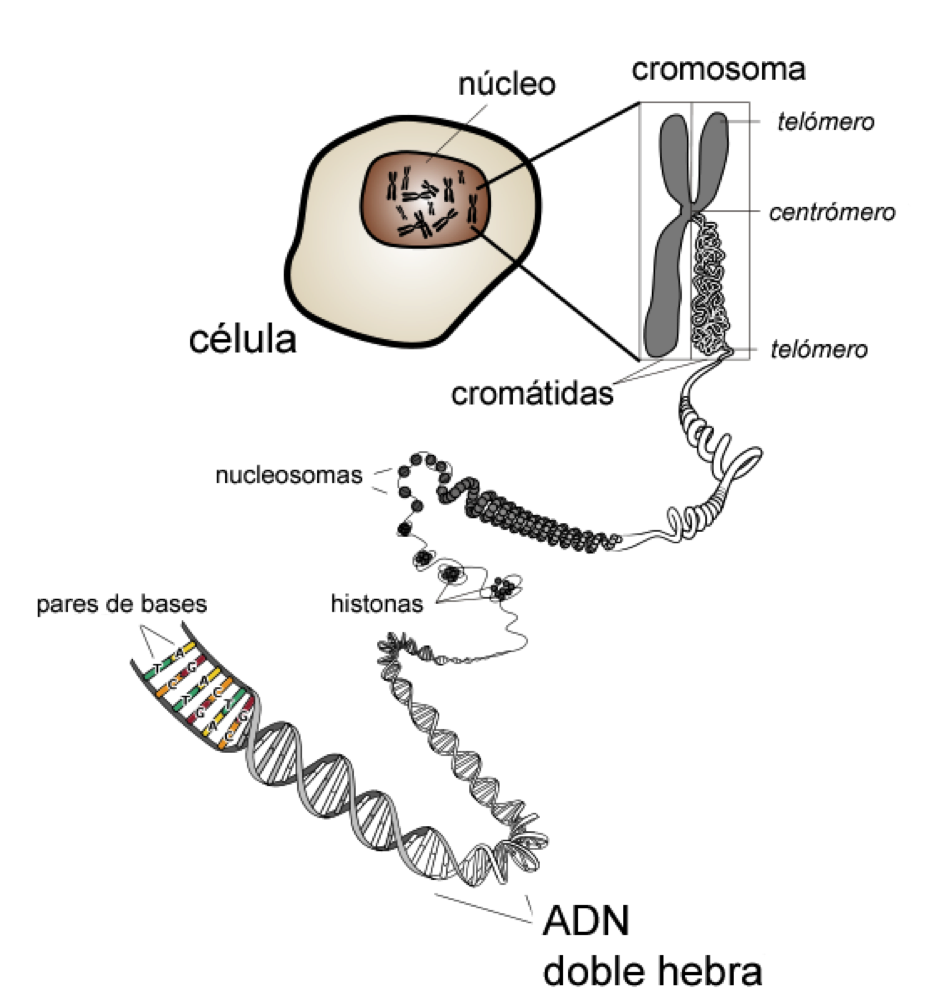
\includegraphics[width=0.45\textwidth]{figs/adn}
\caption{Estructura del ADN.}
\label{fig:adn}
\end{figure}

Sin embargo, existe una diferencia en la información que contiene el código
genético y la expresión del mismo. Eso es lo que llamamos genotipo y fenotipo. El
genotipo es la  información que nuestro código genético contiene. El fenotipo es
la expresión del genotipo. Ésta puede variar por diferentes motivos: dominancia
de genes, medio ambiente, etc. Por ejemplo: es posible tener información para los
ojos azules y marrones y poseer ojos marrones.

Cada individuo de una población tiene su propio ADN único que le define.  No
obstante, no dista mucho de otro individuo de su misma especie. De este modo
pueden reproducirse entre ellos. Esto se debe a que al tener trozos similares de
ADN, con la misma función, se pueden intercambiar por los mismos trozos del otro
individuo. Esto se llama cruzamiento. Así, la descendencia tendrá algunos rasgos
del padre y otros rasgos de la madre: su código genético se ha mezclado
(figura \ref{fig:mendel}).

\begin{figure}[t]
\centering
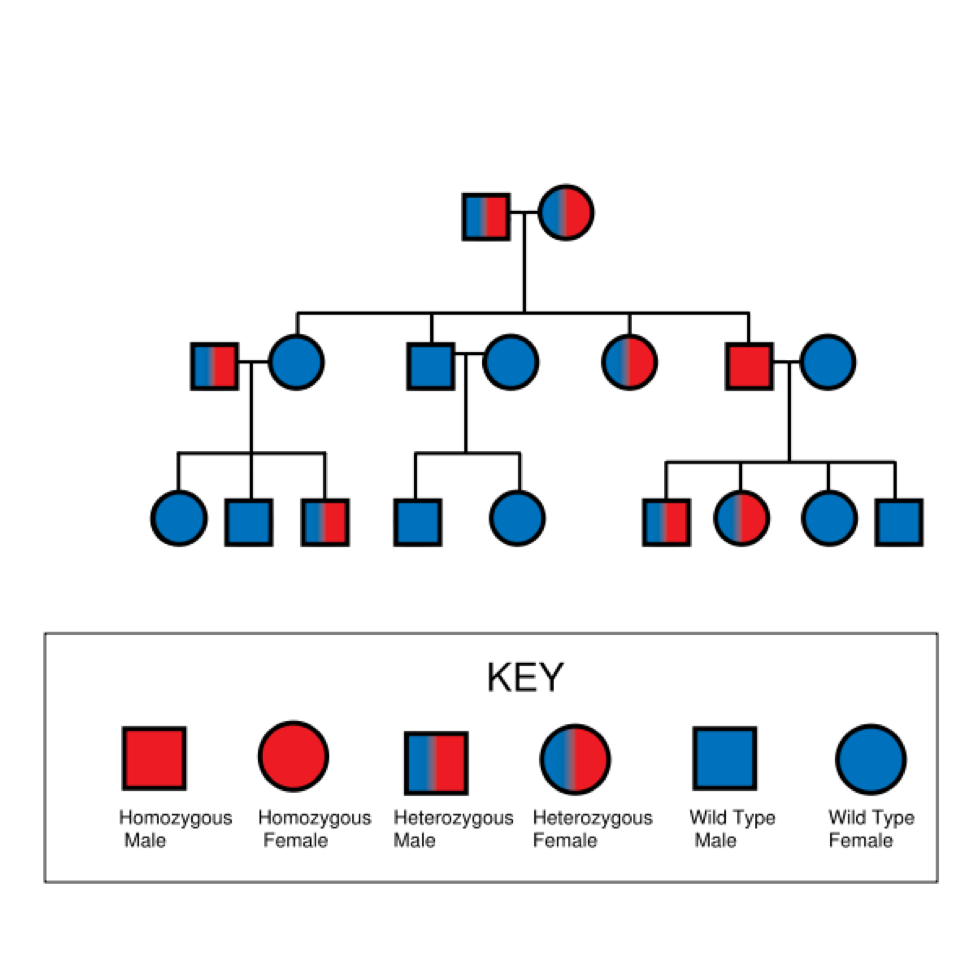
\includegraphics[width=0.45\textwidth]{figs/mendel}
\caption{Ejemplo de posibles descendencias y combinaciones de dos individuos con
dos tipo de gen (rojo y azul).}
\label{fig:mendel}
\end{figure}

Se ha demostrado que la diversidad es necesaria para la supervivencia de la
especie. Este hecho se hizo presente en la realeza Española a lo largo de la
historia, donde solo tenían descendencia entre ellos. La consanguinidad reducía
considerablemente la diversidad genética y empobrecía la calidad de lo
individuos, potenciando enfermedades genéticas. Por ejemplo, Carlos II nació
débil, estéril y enfermizo víctima de sucesivos matrimonios consanguíneos de la
familia real.

Por lo tanto, la naturaleza necesita ciertas similitudes para mezclar ADN, pero,
es fundamental que existan pequeñas diferencias en el ADN de los progenitores.
Esto es crucial para el éxito en la evolución: la diversidad.

La diversidad tiene su origen en la mutación. Una mutación es una alteración en
el código genético que produce cambios en el fenotipo. La consecuencia mas
importante de las mutaciones es que pueden ser heredadas por las siguientes
generaciones. No obstante, la mayoría de las mutaciones producen consecuencias
fatales para el individuo y sólo en contadas ocasiones tienen un resultado
positivo para la continuidad de la especie.  Por ejemplo una mutación que
cambie de color a un animal y por ello es capaz de camuflarse mejor con su
entorno.

La función de la diversidad es crear individuos capaces de ofrecer diferentes
desempeños en situaciones de diversa naturaleza. Estas situaciones pueden ser
fatales si no son superadas. Por ejemplo, el ataque de un determinado virus, o el
ataque de un depredador. Ciertas cualidades consiguen hacer que el individuo siga
viviendo y por lo tanto tener descendencia. Por lo tanto, podríamos decir que la
naturaleza selecciona a los individuos más aptos. Es lo que se llama selección
natural.

Combinando toda esta teoría evolutiva con la informática surge la computación
evolutiva.

\section{Computación evolutiva}

Desde que Von Neumann ideó su modelo de computación moderna en los albores de la
informática, el concepto de algoritmo tomó más fuerza que nunca (una secuencias
de pasos que sirve para resolver un problema). El problema ahora es encontrar la
secuencia de pasos adecuada. Con la ventaja de que estas “nuevas” máquinas eran
capaces de ejecutar estas secuencias de pasos infinitamente más rápido que el ser
humano, se abrió la puerta a nuevos campos de búsqueda y nuevas ideas. Desde
siempre la naturaleza ha aportado a nuestra civilización multitud de ideas y
soluciones y, en este ámbito, no iba a ser diferente. Por qué no imitar el
mecanismo que tiene la naturaleza para dar con sus excelentes soluciones. La
computación evolutiva es la implementación del algoritmo de la evolución.

Esta idea dio lugar a diferentes vertientes dentro de la computación evolutiva,
entonces inexistente como tal. Desde Estados Unidos, J. Fogel  \cite{Fogel:1966}
daba las primeras pinceladas a lo que se llamaría programación evolutiva. Fogel
creó un sistema evolutivo donde los individuos a evolucionar eran máquinas de
estado finito en el ámbito de la predicción. Henry Holland  \cite{Holland:1975}
tuvo otra visión de este concepto y quiso aplicarlo a problemas de optimización,
donde los individuos consistían en valores numéricos que se aplicaban de alguna
forma a un determinado algoritmo. Este método recibió el nombre de algoritmos
genéticos. En 1960 Ingo Rechenberg y Hans--Paul Schwefel  \cite{Rechenberg:1971}
propusieron las Estrategias Evolutivas. Sobre la base de los resultados previos,
Koza  \cite{Koza:1992} inició la última de las cuatro ramas, la programación
genética. En esta última, los individuos que evolucionan son programas informáticos que luchan por
conseguir la solución con mayor (o menor) puntuación.  El mejor programa será
capaz de procrear y tener descendencia, en cambio, los menos aptos estarán
predestinados a desaparecer.

En todas estas ramas es común tener una población de individuos que se reproducen
y/o mutan, permitiendo la descendencia a los individuos que consiguieron mejor
puntuación enfrentándose a un problema determinado. Sorprendentemente, el
algoritmo converge, tendiendo a que la población actual mejore la puntuación de sus
antecesores.

En computación evolutiva es necesario evaluar a cada individuo de la población y
para ello se necesita reproducir el entorno adecuado del problema que se quiere
resolver. Además, para asegurar el éxito de nuestro algoritmo, necesitamos un
gran número de individuos en la población. Esto hace que estos algoritmos
necesiten muchos recursos computacionales. Sin embargo, gracias a los últimos
avances tecnológicos, la computación evolutiva está en auge actualmente.

\section{Programación genética}

En 1992, John R. Koza publicó Genetic Programming: On the Programming of
Computers by Means of Natural Selection \cite{Koza:1992}, un libro que extiende y
asienta las bases que Nichael Lynn Cramer \cite{Cramer:1985} inició con su
publicación A Representation for the Adaptive Generation of Simple Sequential Programs.

Koza habla de las posibles codificaciones que un programa lineal puede tener
 para poder ser evolucionado. Defiende que la estructura más adecuada es la
representación en árbol. Un programa representado como árbol tiene múltiples
ventajas: Es posible volver al estado lineal sin ambigüedades. Las operaciones de
reproducción y mutación consumen menos recursos, además de producir mejor
rendimiento.

Este modelo de representación dio lugar a multitud de alternativas de
modificación y ajuste del algoritmo. Existen infinidad de posibilidades con los
que podemos “jugar” y probar, como los posibles métodos de reproducción,
mutación, inicialización de programas, selección de nodos, etc. Hablaremos de
estos aspectos en los siguientes apartados.

El algoritmo de la programación genética es como todos los algoritmos de la
computación evolutiva. Se trata de un bucle, donde cada iteración se llama
generación. En el caso de la primera iteración se creará una población de un
determinado número de programas aleatoriamente generados. Durante la iteración,
se procederá a la evaluación de los individuos, selección, reproducción,
mutación, y así sucesivamente.

En el proceso de evaluación, se ejecutará el programa y se puntuará de alguna
forma su comportamiento.

En el proceso de selección, se eligen los individuos más aptos de todas la
población para procrear y generar una nueva población. Para procrear se pueden
utilizar diferentes métodos, incluso puede darse el caso en el que los individuos
simplemente se clonen.
 
Una vez que tenemos la nueva población, se forzará la mutación de algunos
individuos con una cierta probabilidad.

El bucle de generaciones llegará a su fin cuando se encuentre al individuo ideal
(si es que puede llegar a existir un individuo que satisfaga todas nuestras
necesidades) o se llegue a un límite de generaciones.



\subsection{El problema del camino de la hormiga (Santa Fe Ant Trail)}

Antes de continuar, se describirá una aplicación de ejemplo muy característico en
la programación genética que servirá para la comprensión de los conceptos. Este
problema es el problema del camino de la hormiga o en inglés Santa Fe Trail Ant.
Consiste en conseguir que una hormiga situada en un mapa de rejilla pueda
seguir el ratro de comida. Este ratro de comida no es continuo. Así la hormiga
tendrá que seguir el ratro a pesar de las discontinuidades (ver figura \ref{fig:santa-fe}).

Evolucionar un individuo que resuelva este problema es un ejercicio de toma de
decisiones. Los individuos reciben información del ambiente; si hay o no comida
en frente de ellos y pueden moverse hacia adelante, girar a la izquierda o
girar a la derecha o una combinación de estos movimientos. El objetivo es comer
toda la comida posible en un periodo de tiempo determinado. Uno de los
motivos por el que se utiliza este problema para introducirnos a la
programación genética es que es sencillo y, sobre todo, mediante la programación
genética se puede resolver fácilmente este problema.


\begin{figure}[t] \centering
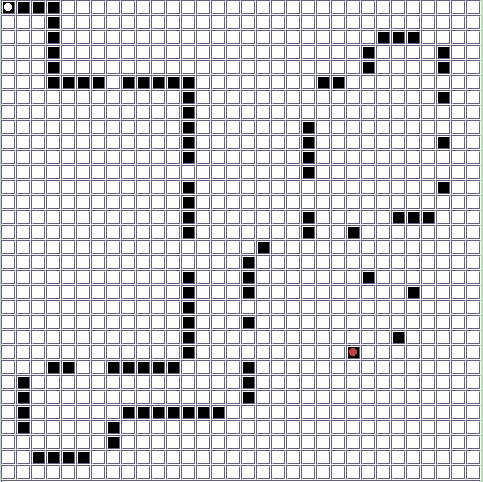
\includegraphics[width=0.65\textwidth]{figs/sftrail}
\caption{Representación del problema del camino de la hormiga de Santa Fe. Los
cuadrados negros representan comida, mientras que los cuadrados blancos están
vacío. El punto blanco es el punto de partida de la hormiga y el punto rojo es
el final del camino.}
\label{fig:santa-fe}
\end{figure}


\subsection{Lenguaje y árboles}

En la programación genética cada individuo tiene una determinada secuencia de
instrucciones a ejecutar, es decir, su propio código genético. Esta secuencia de
instrucciones es, como la propia palabra dice, secuencial. Por ello, muchas
implementaciones de sistemas de programación genética utilizan esta
representación para mezclar y evolucionar programas. Sin embargo, la
representación lineal dificulta las labores de reproducción ya que es difícil
encontrar zonas de similitud para intercambiar código. Asimismo, el intercambio
de código no asegura tener nuevos individuos sintácticamente correctos.

Existe otra forma de representación que aporta mayores alternativas a la hora de
crear y mezclar código genético: la representación en árbol. Es una de las más
extendidas en la programación genética debido a su flexibilidad y al gran número
de posibilidades que ofrece.

Un árbol es una estructura de datos formada por nodos. Un nodo, explicándolo de
una forma informal, es una caja que contiene dentro cierta información y que está
ligada a otras cajas, otros nodos. Estas ligaduras o conexiones se llaman hijos.
Existen nodos que podrán tener varios hijos, y nodos que no tendrán ninguno, en
cuyo caso se les llamará nodos hoja o terminales. Además existirá un nodo base
del que partirán el resto de los nodos (ver figura \ref{fig:arbol}).

\begin{figure}[t] \centering
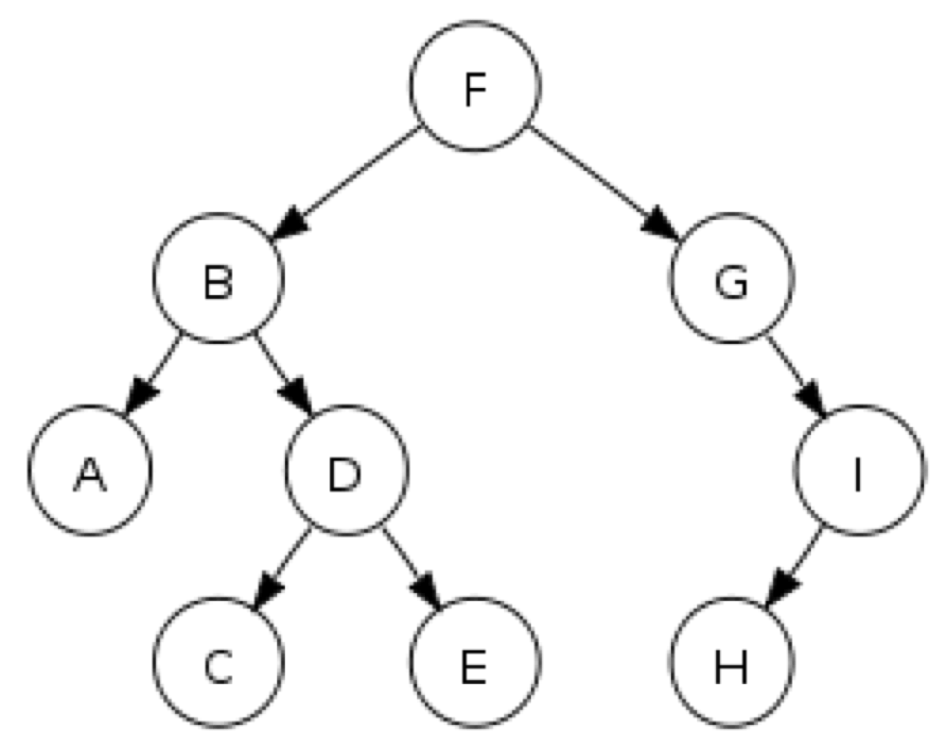
\includegraphics[width=0.45\textwidth]{figs/arbol}
\caption{Representación de un árbol.}
\label{fig:arbol}
\end{figure}

En la programación genética cada nodo contiene una instrucción del programa o una
constante. Las constantes suelen ser nodos terminales, y las instrucciones de
programa suelen ser nodos no-terminales.

Para ejecutar un programa, necesitamos una secuencia de instrucciones. Para
obtener una secuencia de instrucciones de un árbol existen una serie de
transformaciones que transforman estos árboles en un código lineal sin ningún
tipo de ambigüedad. Estas transformaciones se llaman preorder, inorder y
postorder:

Preorder: raíz, subárbol izquierdo, subárbol derecho. (F, B, A, D, C, E, G, I, H)
Inorder: subárbol izquierdo, raíz, subárbol derecho. (A, B, C, D, E, F, G, H, I)
Postorder: subárbol izquierdo, subárbol derecho, raíz. (A, C, E, D, B, H, I, G,
F)


La decisión de utilizar un orden especifico viene dado por el lenguaje que
apliquemos para resolver el problema.

Esta estructura es idónea para la reproducción de los programas, ya que facilita
el proceso de combinación genética que se representa por el intercambio de
subárboles y, en esta estructura, este proceso resulta trivial (cambiar un hijo
por otro).

En la ejemplo de la hormiga, el lenguaje serían todos los movimientos que puede
realizar la hormiga, además de la comprobación de si existe comida frente a ella.
Un pequeño árbol podría ser:

\begin{algorithmic}
\IF {$comidadelante$} 
    \STATE $avanzadefrente$
\ELSE 
	\STATE $avanzalateralmente$
\ENDIF 
\end{algorithmic}

\subsection{Etapas del proceso evolutivo}

El proceso evolutivo es un proceso iterativo, el cual se repite hasta que se
cumpla un criterio de parada. El criterio de parada puede ser que se haya llegado
a un máximo de iteraciones o que se haya encontrado al individuo deseado.

En la primera generación se inicializa la población, mediante procesos aleatorios
que debe proveer a la población de la suficiente diversidad para proporcionar el
éxito del algoritmo.

Después, el proceso iterativo se reduce a tres etapas: selección de individuos,
reproducción y adición de los nuevos individuos.

\subsubsection{Inicialización}\label{subsubsec:inittree}

La inicialización consiste en crear una nueva población y dotar a todos
los individuos de la población de un código genético admisible, además de generar
la diversidad suficiente en la población para que el sistema pueda evolucionar.
Se pueden llevar a cabo multitud de métodos para acometer este fin, sin embargo,
los más empleados y comunes son los métodos grow y  full que se suelen combinan
de forma que el 50\% de la población se genera por el método grow y el restante
con el método full. Estos métodos los describiremos a continuación.

El método grow genera un árbol de programa de un individuo aleatoriamente hasta
una determinada profundidad. En concreto, dado un conjunto de terminales  y de no
terminales de nuestro lenguaje, el método grow va rellenando el árbol
aleatoriamente escogiendo indiferentemente entre terminales y no terminales hasta
llegar a la máxima longitud, en cuyo caso sólo elije terminales terminando con la
expansión del árbol. Aunque existe un límite estipulado de longitud máxima, es
posible que los árboles generados no lleguen en profundidad a ese límite ya que
al escoger entre aleatoriamente entre símbolos terminales y no terminales, puede
darse el caso que aparezcan símbolos terminales podando el crecimiento del árbol.
Incluso es posible que los árboles generados tengan mayor longitud, ya que si
existe una gramática inherente al lenguaje, puede que en el límite de altura solo
podamos escoger símbolos no terminales, prolongando el crecimiento del árbol
hasta que podamos seleccionar terminales. Este método está muy condicionado por
la cantidad de nodos terminales y no terminales de nuestro lenguaje, ya que dado
un lenguaje con un alto número de terminales, la probabilidad de escoger uno
aumenta respeto a la probabilidad de escoger un símbolo no terminal. Esto ocurre
también al contrario.

El método full siempre escoge símbolos no-terminales hasta una determinada
profundidad donde, a partir de ahí, sólo elegirá símbolos terminales. Es por esto
que este método siempre genera árboles de la misma profundidad.
 
Como hemos mencionado antes, normalmente se utilizan ambos métodos para generar
la población inicial por el motivo de que el método grow está condicionado por el
número de terminales y no terminales del lenguaje, pudiéndose generar árboles muy
cortos en el caso que en el lenguaje predominen los símbolos terminales. Este
hecho puede poner en peligro el éxito de la evolución, ya que si los árboles que
generamos son demasiado cortos, la diversidad de la población no sería suficiente
para obtener la solución deseada. Sin embargo, el método full garantiza un mínimo
de altura en lo árboles, pero generando siempre árboles de la misma forma. Es por
esto por lo que se combinan ambos métodos, produciendo un número determinado de
individuos con un método y el resto con el otro.

Por último resaltar que en un lenguaje donde predominen los símbolos
no-terminales, los árboles generados con el método grow serán parecidos a los que
genere el método full.

\subsubsection{Evaluación}

Antes de proceder a la selección, es necesario evaluar a la población. El
proceso de evaluación consiste en ejecutar cada individuo y probar su eficacia
al solucionar el problema. Esa eficacia tendrá que ser codificada para poder
comparar a dos individuos cualquiera y decidir cuál es el mejor de ambos.

Para tomar esta decisión, podemos dar a cada individuo una calificación
numérica de su rendimiento. Una vez que tenemos esta calificación, la toma de
decisiones se simplifica al comparar que programa supera en calificación al otro
programa en cuestión. Además, tenemos que tener en cuenta si queremos maximizar
esta calificación, en cuyo caso, 0 sería el valor del individuo menos apto, e
infinito el individuo más apto; o si queremos minimizarla, en cuyo caso 0
representaría el individuo ideal e infinito el individuo menos apto.  Koza se
inclina a utilizar la segunda versión de calificación. A esta forma de puntuación
se la llamó fitness estandarizado. Además existe una transformación que acota
esta calificación entre 0 y 1, donde 0 sería el individuo peor y 1 el mejor. Esta
última calificación ajustada se la llamó a fitness ajustado. La transformación se
realiza mediante la siguiente formula:
\begin{equation}
   Adj = \frac{1}{1+f},
\end{equation} donde $f$ es el fitness estandarizado.


No obstante, en determinadas ocasiones, es difícil obtener una única nota por individuo, puesto que es posible
que existan diferentes medidas que influyen en la decisión.  Estos problemas surgieron sobretodo cuando se
detectó la aparición de bloat. El bloat son las partes del código del un
programa que carecen de sentido o son innecesarios. Para evitar este fenómeno se quiso introducir una medida más de control del bloat en la toma de decisiones de los individuos. Para combinar estos dos objetivos, se pensó utilizar una combinación lineal de los objetivos del tipo
\begin{equation}
   fitness = \sum_{i}w_if_i(x),
\end{equation}
donde $f_i(x)$ es el valor obtenido al evaluar la $i$-ésima función objetivo y  $w_i$ el valor por el cual
misma se poderará.

Incluso se puede llegar a tener una ponderación exponencial de los objetivos, cuando queremos dar mucha mas
importancia a un objetivo que a otro. Es posible, además, impedir el uso de un determinado objetivo hasta un
cierto nivel de satisfacción de otro objetivo.

Sin embargo, hay que prestar especial atención a la hora de combinar todos nuestros objetivos ya que es posible
que limitemos la evolución de nuestros programas si elegimos unos parámetros incorrectos. Por ello conviene
realizar un estudio previo del rendimiento de nuestro fitness.

Langdon y Poli \cite{LangdonPoli:1998} utilizaron un función semilineal para
combinar el acierto del programa y la velocidad para mejorar el rendimiento de la programación genética en el problema de la hormiga. No obstante, necesitaron
ajustar este fitness para aquellas hormigas que eran muy rápidas pero no conseguían resolver el problema.

Pero la combinación lineal de objetivos no es la única aproximación posible para resolver problemas
multi-objetivo, existen otros métodos capaces de optimizar varios objetivos simultáneamente, por ejemplo,
métodos basados en la optimización de la frontera de Pareto.

La frontera de Pareto es aquella frontera formada por las soluciones óptimas de una población. Estas soluciones
no se pueden comparar ya que, si por ejemplo observamos la figura
\ref{fig:pareto}, en algún punto una solución A ofrece mejor resultado frente a cierto problema que una solución B, sin embargo la B ofrece mejor solución a otro problema que la A. Por ello no se pueden comparar.
Sin embargo puede existir una solución C cuyas soluciones sean peor que la dada por la A, en ese caso, A es
estrictamente superior que C. Este sistema intenta evitar que la solución se quede en un mínimo local, ampliando
las fronteras a otros mínimos de interés. Además tiene la ventaja de potenciar la diversidad.

\begin{figure}[t]
\centering
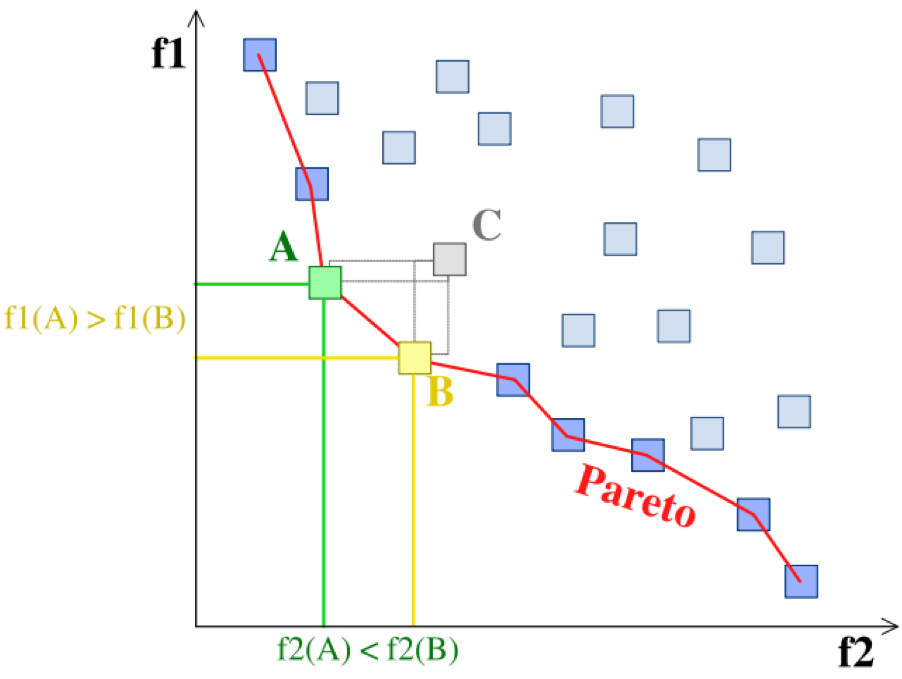
\includegraphics[width=0.65\textwidth]{figs/pareto}
\caption{Ejemplo de la frontera de Pareto.}
\label{fig:pareto}
\end{figure}

Además de la frontera de Pareto, existen otros métodos como el orden lexicográfico (los objetivos son ordenados
según la preferencia del usuario),  métodos basados en prioridades, otros métodos basados en la dominancia de la
frontera de Pareto pero con la adhesión de la cuenta del número de objetivos que un individuo es mejor que otro.
Incluso, es posible combinar varios métodos de evaluación, para conseguir una visión más objetiva y diversa
del problema. 

\subsubsection{Selección}

El proceso de selección sirve para escoger a los individuos de la población mejor
adaptados, para que actúen de progenitores de la siguiente generación. En la
naturaleza existen varios factores que intervienen para que un individuo pueda
tener descendencia. El primero de todos es que consiga sobrevivir, ya sea por que no es
devorado por depredadores, o porque sea capaz de procurarse alimento. Lo segundo
es que encuentre pareja para reproducirse. El último factor es que la
combinación de ambos individuos sea apta para crear un nuevo individuo. Sin
embargo, en la realidad es posible que “el mejor” individuo no pueda
reproducirse, pero otro individuo de “peor calidad” pueda conseguirlo. Aunque
este hecho es menos probable, sigue siendo posible.

En la programación genética, la selección es un conjunto de reglas que sirven para elegir a los progenitores de
la siguiente generación. Estos progenitores se reproducirán (cruzamiento genético) y generarán descendencia.

Un sistema muy utilizado en programación genética es la selección por torneo (tournament selection).  Este
sistema consiste en escoger aleatoriamente de la población un cierto número de individuos. De esos individuos se
escoge el mejor de todos para ser el padre. Para escoger la madre se repite el proceso: se escoge aleatoriamente
a un número de individuos de la población y se elige al individuo con mejor calidad. Este sistema garantiza un
mínimo de diversidad, ya que no siempre se elegirá al mejor individuo de la población para tener descendencia y
por lo tanto, no todos los hijos tendrán al mismo padre. Pero, por el contrario, existen grandes posibilidades
de que éste tenga descendencia, ya que si es escogido en algún torneo, será el vencedor.

Además existen otros métodos que no solo tienen en cuenta si un individuo es mejor que otro, sino que miden
también la diferencia de la calidad, ya que si la diferencia no es muy grande, quizás el vencedor de la
selección no es el que tenga un desempeño estrictamente superior.


\subsubsection{Reproducción}

La fase de reproducción es la que se encarga de generar nuevos individuos,
preferiblemente diferentes, a partir de los predecesores seleccionados en el
proceso anterior. En esta fase se pueden utilizar varios métodos de reproducción.
El cruzamientos es un método que consiste en intercambiar parte del código del
padre y parte del de la madre. Otro método más simple es el de la clonación, cuya
función consiste en copiar a los progenitores en la nueva población. Además, para
generar más variedad, los individuos son mutados con cierta probabilidad, esto es
que el código genético de algunos individuos es modificado introduciendo nuevo
material genético dentro de la población (figura \ref{fig:cross}).

\begin{figure}[t]
\centering
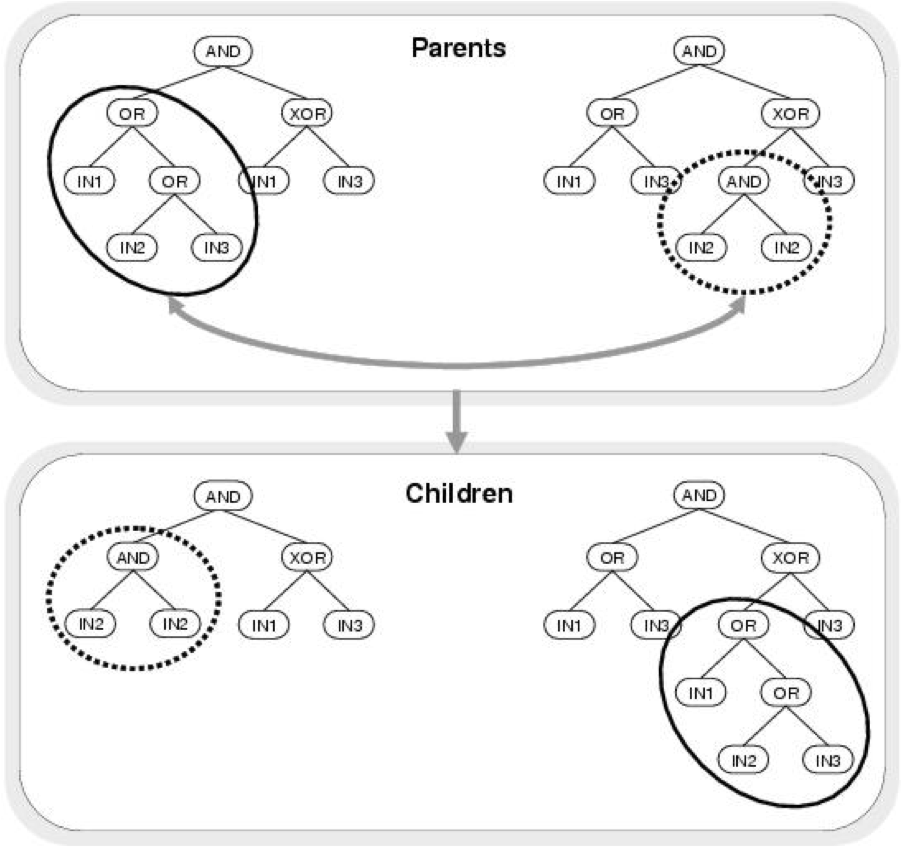
\includegraphics[width=0.55\textwidth]{figs/cross}
\caption{Cruzamiento de dos árboles.}
\label{fig:cross}
\end{figure}

Dependiendo del problema, nos interesará utilizar cruzamiento o clonación y mutación, o una combinación de estos
operadores controlados por probabilidades de aparición.
 
\paragraph{Cruzamiento}\label{para:crossover}

El cruzamiento es el intercambio de material genético entre dos individuos para producir un individuo nuevo y
diferente. En programación genética esto se traduce en intercambio de subárboles. Cuando dos individuos se van a
reproducir se selecciona un nodo aleatoriamente en el padre y otro nodo en la madre y se realiza el intercambio
de subárboles.

Sin embargo, en la naturaleza, durante la reproducción sexual de dos individuos se intercambia parte del código
genético de tal forma que el nuevo código genético generado es similar al de los padres. Esto es posible debido
a la organización existente del código genético en genes y cromosomas. En la programación genética  no sucede
exactamente de la misma forma ya que resulta muy costoso identificar las partes de código similares entre dos
programas. Es por ello que el código genético se almacena en árboles, imitando los genes y cromosomas en la
naturaleza. De esta forma se consigue estructurar el código genético de tal forma que puedan encontrarse partes
similares fácilmente. No obstante, la simple estructuración del código genético del programa en árboles no es
suficiente y requiere de subprogramas adicionales que controlen la reproducción ya que el intercambio de
subárboles sin control mismo puede cambiar radicalmente la configuración del árbol resultante, produciendo
efectos fatales.

Existen varios métodos denominados métodos homólogos que intentan preservar la
posición del material genético. Mantener la posición física del material
genético es trivial cuando se trata de programas lineales ya que en su forma
natural ya son lineales. Sin embargo, este proceso resulta más tedioso cuando
el código se encuentra almacenado en árboles ya que la transformación a código
lineal puede verse afectada enormemente por un ligero cambio en el arbol.

El más viejo operador de cruzamiento homólogo en programación genética es el
cruzamiento en un punto. El operador intercambia un subárbol que coincida en la
raíz en los dos padres. Identifica las partes con la misma forma estructural
(misma aridad\footnote{En el análisis matemático, se define a la aridad de un
operador matemático o de una función como el número de argumentos necesarios para
que dicho operador o función se pueda calcular.}), e intercambia el código
genético a partir de estas partes comunes. De esta forma, este sistema intenta
mantener la posición original del código genético intercambiado
\cite{LangdonPoli:2002}.

El método de cruzamiento de tamaño similar escoge el primer nodo de forma aleatoria como el cruzamiento normal.
Sin embargo, el segundo nodo debe seleccionarse de tal forma que la altura de este segundo subárbol debe ser
parecida a la altura del primer subárbol seleccionado.
 
Harries y Smith \cite{HarriesSmith:1997} idearon cinco operadores nuevos de
cruzamiento muy parecidos a los tradicionales pero con restricciones de profundidad en los puntos de cruzamiento de los árboles de los padres utilizando un criterio
probabilístico.

No obstante, existen otras clases de operadores lineales de cruzamiento, pero pertenecen a una representación
distinta a la utilizada, por lo que no nos concierne para el desarrollo del proyecto. 

\subparagraph{Clonación}

Como su propio nombre dice, se trata de copiar individuos de una generación a otra. Este método se llama también
reproducción, aunque en este contexto el nombre puede dar lugar a ambigüedades. Clonar no aporta nueva
diversidad a la población, no obstante, en ciertas ocasiones resulta conveniente aplicarlo, sobre todo en las
ocasiones donde se ha conseguido una solución muy óptima y no se desea perder la información correspondiente a
esa solución.

Al ser un operador que pone en peligro la diversidad de la población se suele utilizar con probabilidades muy
bajas o nulas. Por otro lado, es cierto que en la naturaleza existen especies que utilizan la clonación como
forma de reproducción, pero siempre se da en organismos sencillos. Por otro lado, existen estudios que
demuestran que posible evolucionar individuos con clonación combinada con mutación.

Por otro lado existe un sistema de los algoritmos evolutivos llamado elitismo que es un mecanismo para preservar
a los individuos más aptos de la población clonando a estos individuos en la nueva población.


\subparagraph{Mutación}

En el ámbito de la programación genética la mutación se define como el cambio aleatorio del código genético
(código de programa) del individuo. Este cambio se puede producir en cualquier punto del código y actuar de las
siguientes formas: borrando código, generando código o cambiando una instrucción por otra.

La mutación, al producirse de forma aleatoria, produce efectos incontrolados y genera individuos menos aptos
para la supervivencia. Por ello, la frecuencia de aparición de este fenómeno suele ser baja. Incluso se ha
llegado a cuestionar si es necesario para que el algoritmo evolutivo converja. Se ha demostrado que es posible
resolver problemas con programación evolutiva sin llegar a utilizar la mutación. Sin embargo, la mutación debe
entenderse como un punto de entrada de diversidad. Y si no somos capaces de generar esa diversidad en el inicio
del algoritmo, la mutación salvará a la población de quedarse estancada.

A diferencia de los programas lineales donde una mutación solo produce un cambio puntual en el material
genético, las mutaciones en los árboles pueden aparecer de diversas formas, que se explican a continuación:

 \begin{enumerate}
    \item La mutación de subárbol selecciona un nodo aleatoriamente y genera un
    subárbol aleatorio para ese nodo \cite{Koza:1992}.
    Kinnear \cite{Kinnear:1993} amplió este método restringiendo la profundidad
    del árbol producido a un 15\%.

	\item La mutación de reemplazo de nodo selecciona un nodo al azar y lo
	reemplaza por un nodo equivalente, de la misma aridad y mismas propiedades. Este método se parece a la versión lineal de reemplazar una línea de código
por otra.

	\item La mutación Hoist genera un nuevo individuo a partir de un subárbol del
individuo anterior. La raíz del nuevo árbol será diferente al del anterior y el árbol generado será más pequeño.

	\item La mutación Shrink intercambia un subárbol elegido aleatoriamente por un
nodo terminal aleatorio compatible. Este método también reduce el tamaño final del programa.


	\item La mutación de permutación selecciona un nodo aleatoriamente e
intercambia de posición sus subárboles. Es posible que en algunos casos, este intercambio no refleje ningún cambio en el funcionamiento del programa.

\end{enumerate}

\subsubsection{La nueva población}

Una vez que hemos seleccionado, reproducido y con cierta probabilidad mutado la
población, es el momento de generar otra población con nuevos individuos.
Normalmente se escogen los nuevos individuos más aptos y se rellena la población
hasta un número máximo de individuos. Además, se puede reservar un espacio de
esta población para los individuos más aptos, con mejor puntuación, de la
generación anterior. Esto se llama elitismo. Aunque el elitismo apueste en contra
de  la diversidad, se ha comprobado que en ciertas ocasiones acelera la
convergencia del algoritmo, sin embargo, debe utilizarse con precaución. Además
al crear esta nueva población podemos encontrar dos formas de hacerlo: El modo
generacional y el modo de estado estacionario.

En el modo de estado generacional el sistema almacena todas las generaciones en espacios diferentes. Los nuevos
individuos ocupan un nuevo espacio. Este modo evolutivo aporta un gran valor
estadístico e incluso sería posible que antiguos individuos interviniesen en
nuevas poblaciones ya que poseemos la información de todos los
individuos de la evolución. El único inconveniente de este sistema es que requiere muchos más recursos y puede
ser un modo poco factible para largas ejecuciones.

En el modo de estado estacionario, el espacio asignado para almacenar los
programas siempre es el mismo, de esta forma, los nuevos individuos tienen que
desplazar a los individuos antiguos, ocupando su posición. Este método resulta
ideal para ejecuciones muy largas, poblaciones muy extensas o individuos que
ocupen mucho espacio en memoria. Incluso, es posible que en determinadas
ocasiones, el sistema ofrezca un rendimiento más alto que el sistema
generacional, ya que no tiene que generar nuevas estructuras, ni preocuparse por
clonar los individuos antiguos para crear nuevos. Lo único que tiene que hacer es
mantenerlos en la población.

\subsection{El cubo de Rubik}

El cubo de Rubik fue inventado por un profesor de arquitectura Húngaro Ernö Rubik
en 1974. Se trata de un puzzle en forma de cubo de 6 caras y con 9 pegatinas
coloreadas en cada cara.  Cada cara tiene un color y estas caras se pueden rotar
descolocando las posiciones de los colores. El objetivo del juego es volver a
juntar las pegatinas del mismo color.

La dificultad del cubo de Rubik radica en las millones de posiciones diferentes
que puede llegar a tener. En total se calcula que pueden existir más de 43
millones de permutaciones \cite{wiki:Rubik}.

Existen diversas formas de resolución del cubo de Rubik, no obstante, el misterio está en que no es posible
formalizar un algoritmo capaz de encontrar una solución óptima (la que menos pasos requiere) de cualquier cubo
desordenado. En 2008, Tomas Rokicki  \cite{Rokicki:2008} estableció el record
mas reciente y demostró que cualquier cubo de Rubik se resuelve en 22 movimientos o menos.

Estos algoritmos se basan en la búsqueda de todo el espacio de posibilidades del cubo de Rubik, el cual, es tan
grande que se puede tardar varias décadas en calcular. Para simplificar ligeramente el proceso se utiliza la
descomposición matemática del cubo de rubik en subconjuntos. Estos subconjuntos son más fáciles de resolver y
ofrecen una guía para estos algoritmos.

En nuestro sistema solo vamos a poder realizar movimientos de caras. Por lo tanto ya que tenemos 6 caras y dos
sentidos de movimientos, podremos hacer 12 movimientos en cada estado. Si tenemos un cubo ordenado, podremos
hacer 12 desplazamientos. Estos 12 cubos diremos que pertenecen a la dificultad 1. Por cada uno de estos 12
cubos tendremos 12 movimientos, por lo tanto 144 posibilidades. Estos cubos pertenecerán al nivel 2. Nótese que
12 de estos 144 cubos, es el cubo resuelto. Del nivel 3 tendremos 1.728 cubos y así en adelante.

Estos niveles de dificultad nos servirán para clasificar los cubos de Rubiks y tener una noción a priori del
número de pasos que son requeridos para su resolución.

Para referirnos a las caras del cubo utilizaremos la nomenclatura desarrollada
por David Singmaster  \cite{Singmaster:1981}:

\begin{itemize}
  \item F(Front): la cara que de enfrente. 
  \item B(Back): la cara opuesta a la frontal. 
  \item U(Up): la cara de encima a la frontal. 
  \item D(Down): la cara de debajo de la frontal.
  \item L(Left): la cara a la izquierda de la frontal. 
  \item R(Right): la cara a la derecha de la frontal.
\end{itemize}

Esta nomenclatura estandariza el caso de los posibles movimientos del cubo y hace posible expresar una posible
solución de forma rigurosa y sin ambigüedades.
\chapter{Objetivos del PFC}\label{ch:objetivos}

El objetivo del proyecto de fin de carrera consiste en evolucionar un programa a
través de la programación genética capaz de resolver el cubo de Rubik de forma
óptima. Como este objetivo es realmente amplio, se dividirá en varios
subobjetivos:

\section{Encontrar un lenguaje apropiado para representar la solución del
problema}

El lenguaje que utilice nuestro programa necesitando pocos nodos, será capaz  de
expresar un solución. Cuanto menos nodos tenga que generar la programación, la
soluciones serán menos complejas, por lo tanto, la convergencia del algoritmo
será más alta, llegando a una solución más rápidamente.

\section{Encontrar un fitness adecuado para que nuestro sistema evolutivo
consiga desarrollarse y generar soluciones del cubo de Rubik.}

La elección del fitness es fundamental para la correcta evolución del sistema.
Tiene que mantener “sana” la población y a la vez indicar claramente qué
individuos son mejores que otros.

\section{Encontrar un algoritmo de evaluación que obtenga datos
suficientes para determinar el rendimiento del programa.}

El algoritmo de evaluación se encargará de probar el programa con una muestra
representativa del problema, lidiando con factores de eficiencia y rendimiento,
para conseguir en el menor tiempo posible sacar una muestra fiable de las
capacidades del programa evaluado.

\section{Encontrar los parámetros adecuados de nuestro framework para optimizar el
desarrollo del resolvedor.}

Nuestro framework de trabajo contiene infinidad de parámetros a configurar, los
cuales requieren ser correctamente establecidos, ya que una mala configuración
puede ser fatal y generar programas inoperativos. La configuración es crucial
para el éxito de nuestro sistema evolutivo.

\section{Optimizar la velocidad de evaluación.}

Para poder obtener soluciones en un tiempo razonable, el sistema tendrá que
ahorrar cualquier tiempo de CPU extra. Para ello se necesitará crear multitud de
cachees y mecanismos que eviten la repetición de procesos que dan lugar al mismo
resultado ya calculado anteriormente.

\section{Resolver cualquier cubo de Rubik.}

Dentro del objetivo del proyecto, antes de conseguir encontrar una solución
óptima al problema, necesitaremos encontrar una solución cualquiera del problema.
Y, a partir de ahí, reducir el número de pasos a realizar para resolver el cubo.

\section{Buscar las soluciones más compactas.}

Una vez que tenemos la solución al problema, los programas tendrán que ir bajando
la complejidad de sus soluciones hasta llegar a un cierto limite. Obviamente se
desconoce cual es éste, sin embargo, nuestro límite será el tiempo que
dispongamos para encontrar una solución menor. Además llegará un punto en el que
apenas mejore. En ese punto podremos dar por finalizada la ejecución.

\chapter{Diseño del algoritmo}\label{ch:diseno-algoritmo}


\section{Lenguaje}\label{sec:lenguaje}

En este apartado iremos pasando por todos los lenguajes que se han diseñado y
probado hasta llegar al lenguaje escogido para la representación del problema. Un
lenguaje candidato tiene que poder realizar todos los movimientos posibles del
cubo de Rubik y a la vez tiene que realizar las comprobaciones suficientes para
determinar qué movimiento realizar en cada momento. Es por ello que el lenguaje
constará de sentencias condicionales, capaces de ejecutar una rama si la
condición se cumple y sentencias de acción como puede ser el desplazamiento de
una cierta cara en un cierto sentido.

\subsection{Solución 1: El cubo como mapa}\label{subsec:solucion1}

El primer lenguaje que se nos planteó, fue al imaginar un lenguaje parecido al
lenguaje del problema de la hormiga. El problema de la hormiga tiene los
operadores de movimiento de la hormiga por el mapa y las comprobaciones de
existencia de comida enfrente. Adaptando este problema a nuestro problema,
podríamos pensar en el cubo de Rubik como un mapa bidimensional. Un mapa con
forma de cruz, donde cada casilla del cubo representa una posición del mapa.
Sobre este mapa nos podemos mover hacia arriba, hacia abajo, derecha e izquierda.
Al situarnos en el borde de una cara y avanzar nos situaremos en la siguiente
cara, es decir, no existe límite, siempre podemos avanzar.

Una vez que nos podemos desplazar por el mapa, como la hormiga, querremos
realizar ciertas comprobaciones en relación a nuestra posición actual, como por
ejemplo si existe comida en nuestra posición. En el caso del cubo de rubik,
querremos  comprobar el color de la pegatina en la que estemos situados.

Una vez que tenemos la funcionalidad de comprobar cualquier casilla de nuestro
cubo de Rubik, los siguientes operadores son triviales y básicos para el
resolvedor del cubo de Rubik: los movimientos de cara. Estos son los operadores
que rotan una cara, por ejemplo, el que rota la cara derecha en sentido de las
agujas del reloj.

Es normal pensar qué parámetros son necesarios en nuestro sistema, es decir,
cuando movemos una cara necesitaremos especificar qué cara movemos. Debe existir
el operador “mover” y el parámetro “cara” que especifica que cara movemos. No
obstante, el objetivo de este lenguaje es conseguir un lenguaje gramaticalmente
libre, de tal forma que cualquier nodo sea compatible con otro.

Este hecho tiene la ventaja de que cualquier nodo puede sustituir a otro, por
eso, los operadores de mutación y cruzamiento requieren de menos esfuerzo para
llevar a cabo con éxito su labor. Por lo tanto, en el lenguaje tendremos nodos
del tipo “IfBlue”, “IfRed” o MoveFaceUpClockwise.

De esta forma tenemos el conjunto de nodos terminales que se muestra en la
tabla \ref{tab:n-terminales-sol1} y en la figura \ref{fig:leng1nodosterm}, y el
conjunto de nodos no-terminales en la tabla \ref{tab:n-noterminales-sol1} y en
la figura \ref{fig:leng1nodosnoterm}.


\begin{table}[t]
\caption{Tabla de nodos terminales de la solución 1.}
\label{tab:n-terminales-sol1}
\centering
\begin{tabular}{lp{8cm}}
\toprule
\textbf{Nombre} & \textbf{Descripción}\\
\midrule
\textbf{MovePosUp}					&	Mueve la posición actual a la casilla superior. Si no
existe tal casilla, se saltará de cara a la superior a la casilla Y2. Si
estamos en la cara superior, nos desplazaremos a la cara trasera.\\ \hline
\textbf{MovePosDown}				&	Mueve la
posición actual a la casilla inferior. Si no existe tal casilla, se saltará de
cara a la inferior a la casilla Y0. Si estamos en la cara inferior, nos
desplazaremos a la cara trasera.\\\hline
\textbf{MovePosLeft}				&	Mueve la posición actual a la casilla izquierda. Si
no existe tal casilla, se saltará de cara a la izquierda a la casilla
X2.\\\hline \textbf{MovePosRight}				&	Mueve la posición actual a la casilla derecha. Si no
existe tal casilla, se saltará de cara a la derecha a la casilla X0. \\\hline
\textbf{MoveFaceUpClockwise}			&	Mueve la cara superior en el sentido de las
agujas del reloj.\\\hline
\textbf{MoveFaceDownClockwise}		&	Mueve la cara inferior en el sentido de las
agujas del reloj.\\\hline
\textbf{MoveFaceRightClockwise}		&	Mueve la cara derecha en el sentido
de las agujas del reloj.\\\hline
\textbf{MoveFaceLeftClockwise}		&	Mueve la cara izquierda en
el sentido de las agujas del reloj.\\\hline
\textbf{MoveFaceFrontClockwise}		&	Mueve la cara
frontal en el sentido de las agujas del reloj. \\\hline
\textbf{MoveFaceBackClockwise}		&	Mueve la cara trasera en el sentido de las
agujas del reloj.\\\hline
\textbf{MoveFaceUpCounterClockwise}&	Mueve la cara superior en el sentido
opuesto a las agujas del reloj.\\\hline
\textbf{MoveFaceDownCounterClockwise}&	Mueve la cara inferior en
el sentido opuesto a las agujas del reloj.\\\hline
\textbf{MoveFaceRightCounterClockwise}&	Mueve
la cara derecha en el sentido opuesto a las agujas del reloj.\\\hline
\textbf{MoveFaceLeftCounterClockwise}&	Mueve la cara izquierda en el sentido
opuesto a las agujas del reloj.\\\hline
 \textbf{MoveFaceFrontCounterClockwise}&	Mueve la cara frontal en
el sentido opuesto a las agujas del reloj.\\\hline
 \textbf{MoveFaceBackCounterClockwise}&Mueve
la cara trasera en el sentido opuesto a las agujas del reloj.\\
\bottomrule
\end{tabular}
\end{table}


\begin{table}[t]
\caption{Tabla de nodos no-terminales de la solución 1.}
\label{tab:n-noterminales-sol1}
\centering
\begin{tabular}{lcp{8cm}}
\toprule
\textbf{Nombre}&\textbf{Aridad}& \textbf{Descripción}\\
\midrule
\textbf{IfBlue}&2&	Comprueba que la casilla de la posición actual sea azul. Si
es así ejecuta lo hijos de la izquierda. Si no, ejecuta los de la
derecha.\\\hline
\textbf{IfWhite}&	2& Comprueba que la casilla de la posición actual sea blanca.
Si es así ejecuta lo hijos de la izquierda. Si no, ejecuta los de la
derecha.\\\hline
\textbf{IfGreen}&2& Comprueba que la casilla de la posición actual sea verde.
Si es así ejecuta lo hijos de la izquierda. Si no, ejecuta los de la derecha.
\\\hline
\textbf{IfOrange}&	2&	Comprueba
que la casilla de la posición actual sea naranja. Si es así ejecuta lo hijos de
la izquierda. Si no, ejecuta los de la derecha.\\ \hline
\textbf{IfRed}&	2&	Comprueba que la
casilla de la posición actual sea rojo. Si es así ejecuta lo hijos de la
izquierda.Si no, ejecuta los de la derecha.\\\hline
\textbf{IfYellow}&	2&	Comprueba que la
casilla de la posición actual sea amarillo. Si es así ejecuta lo hijos de la
izquierda. Si no, ejecuta los de la derecha. \\\hline
\textbf{Progn2}&	2&	Ejecuta primero la rama
izquierda y luego la derecha.\\\hline
\textbf{Progn3}&	3&	Ejecuta primero la rama izquierda,
luego la central y luego la derecha.\\
\bottomrule
\end{tabular}
\end{table}


\begin{figure}[t]
\centering
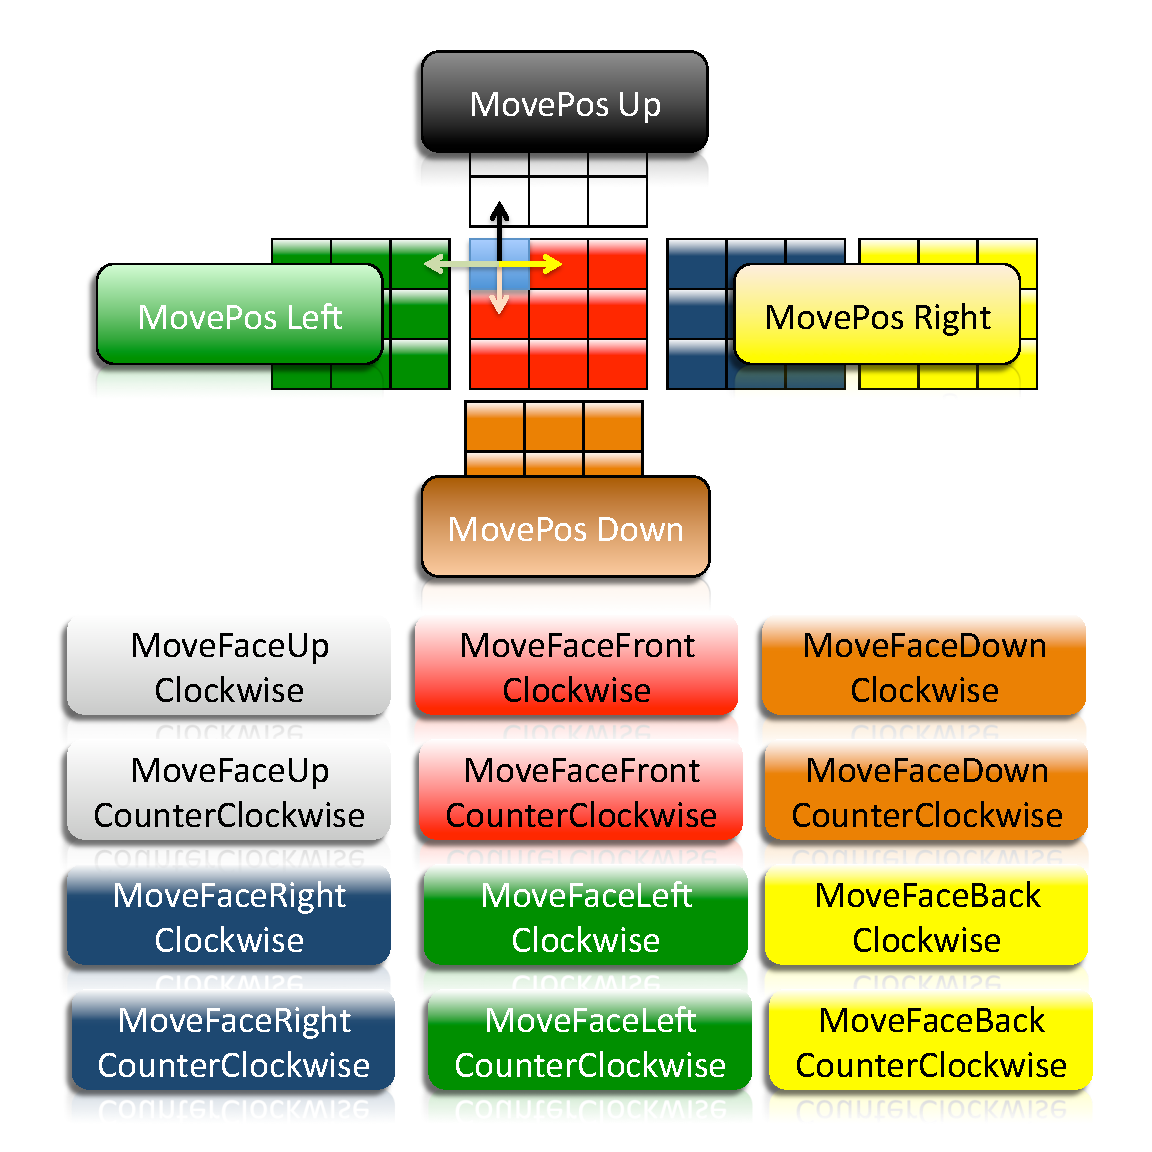
\includegraphics[width=0.65\textwidth]{figs/pdf/leng1nodosterm}
\caption{Nodos terminales de la solución 1.}
\label{fig:leng1nodosterm}
\end{figure}

\begin{figure}[t]
\centering
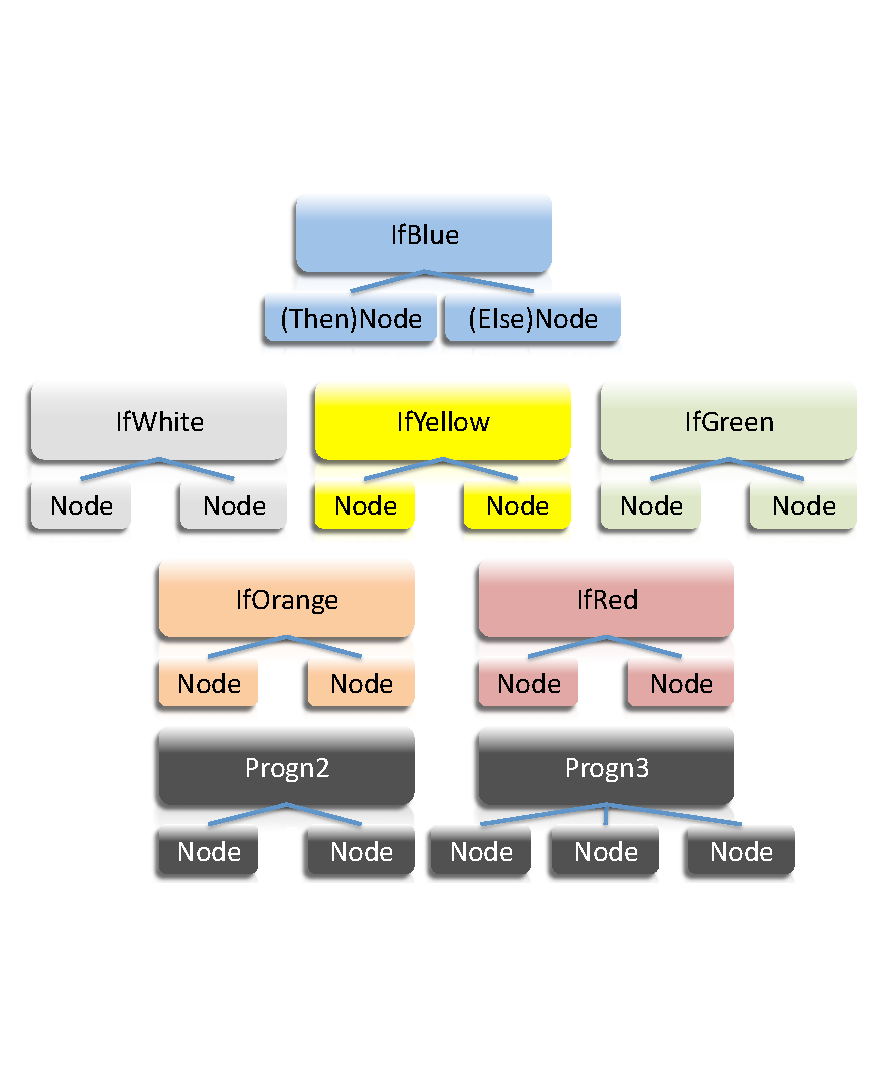
\includegraphics[width=0.65\textwidth]{figs/pdf/leng1nodosnoterm}
\caption{Nodos no terminales de la solución 1.}
\label{fig:leng1nodosnoterm}
\end{figure}



Este lenguaje ofrece la ventaja que cada nodo es sustituible por cualquier otro.
De esta manera, la generación de árboles, cruzamiento, mutación y cualquier
operador que trabaje con el lenguaje resultará beneficiado de esta situación.

Sin embargo este lenguaje resulta poco eficiente, en cuanto al número de nodos
requeridos para lograr resolver cubos, ya que el trabajo que cuesta comprobar dos
casillas diferentes no siempre es el mismo, de modo que alcanzar el camino hacia
una casilla puede convertirse en otro problema de cierta complejidad en si mismo.

Además, al ser necesario saber en que posición estamos, es inherente que el
estado del sistema entre en juego a la hora de determinar los resultados de un
operador. Es por esto que este lenguaje es difícilmente predecible y entendible
por el hombre.

Por otra parte, este es un lenguaje débilmente tipado de forma que la aparición
de bloat estará mucho más presente, y podrá ocupar un espacio mucho mayor en los
árboles del sistema.

Vamos a ver un ejemplo de cómo se podría solucionar un cubo de Rubik de nivel 1
(una cara desplazada respecto de la solución, figura \ref{fig:leng1ejemplo1})
con este lenguaje. Si, por ejemplo, rotamos la cara de la izquierda en el sentido de las agujas del reloj, tendremos
un cubo de Rubik de nivel 1, donde la cara frontal tiene tres casillas del color
de la cara superior, la cara inferior tiene 3 casillas del color de la cara
frontal y así sucesivamente. Para dar con la solución bastaría con el siguiente
plan:

\begin{algorithmic}
\IF {$Orange$} 
        \STATE $MovePosDown$
        \STATE $MovePosDown$
        \STATE $MovePosDown$
        \STATE $MovePosRight$
        \IF {$Orange$}
                \STATE $MoveFaceLeftCounterClockwise$
        \ENDIF
\ENDIF 
\end{algorithmic}

El plan puede no parecer muy complicado, pero si queremos volver a evaluar la
casilla inicial, tendremos que volver hacia atrás y repetirlo del mismo modo con
todas las casillas que se tengan que comprobar. Por otra parte, el lenguaje
admite sentencias del tipo 
\begin{algorithmic}
\IF {$IfOrange$} 
        \IF {$IfRed$}
                \STATE \ldots
        \ENDIF
\ENDIF 
\end{algorithmic} 
(figura \ref{fig:leng1ejemplo2}) que carecen de sentido y que son
difícilmente controlables. Esto puede desencadenar la generación de mucho código
sin sentido que carezca de utilidad.




\begin{figure}[t]
\centering
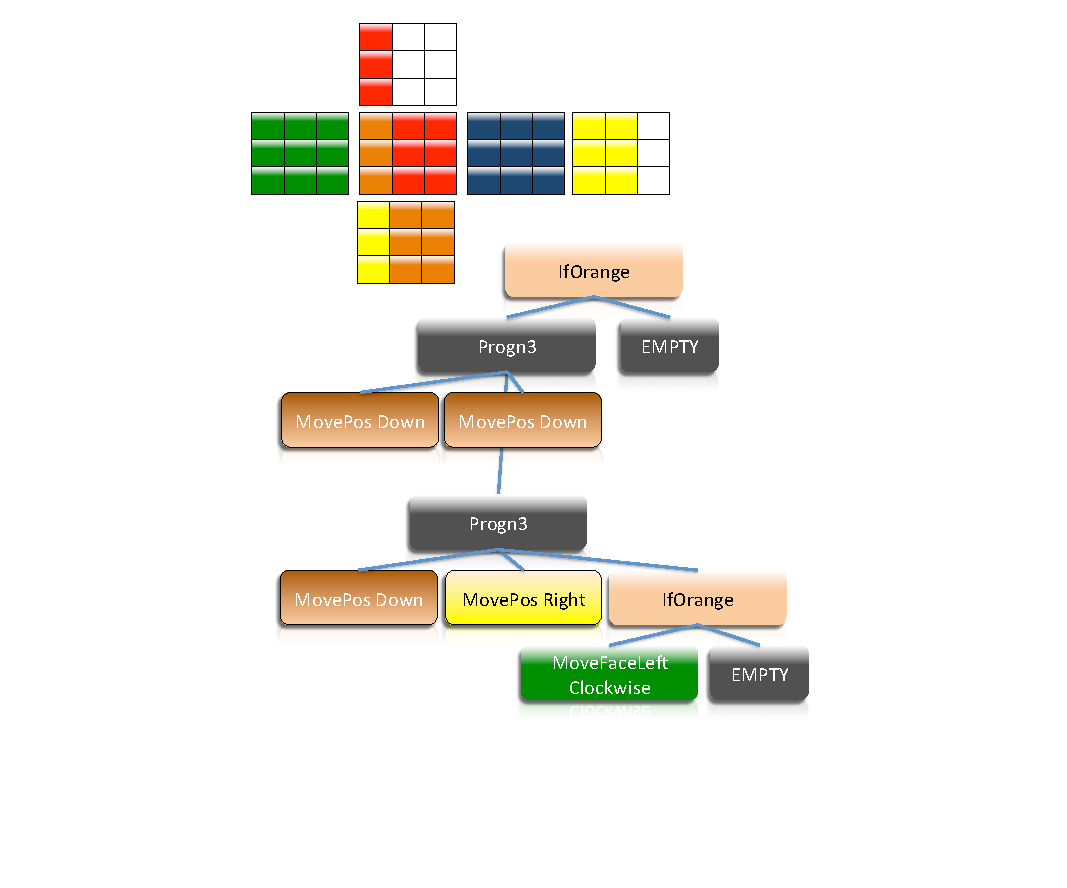
\includegraphics[width=0.65\textwidth]{figs/pdf/leng1ejem1}
\caption{Ejemplo de árbol que resuelve un cubo de rubik de nivel 1.}
\label{fig:leng1ejemplo1}
\end{figure}

\begin{figure}[t]
\centering
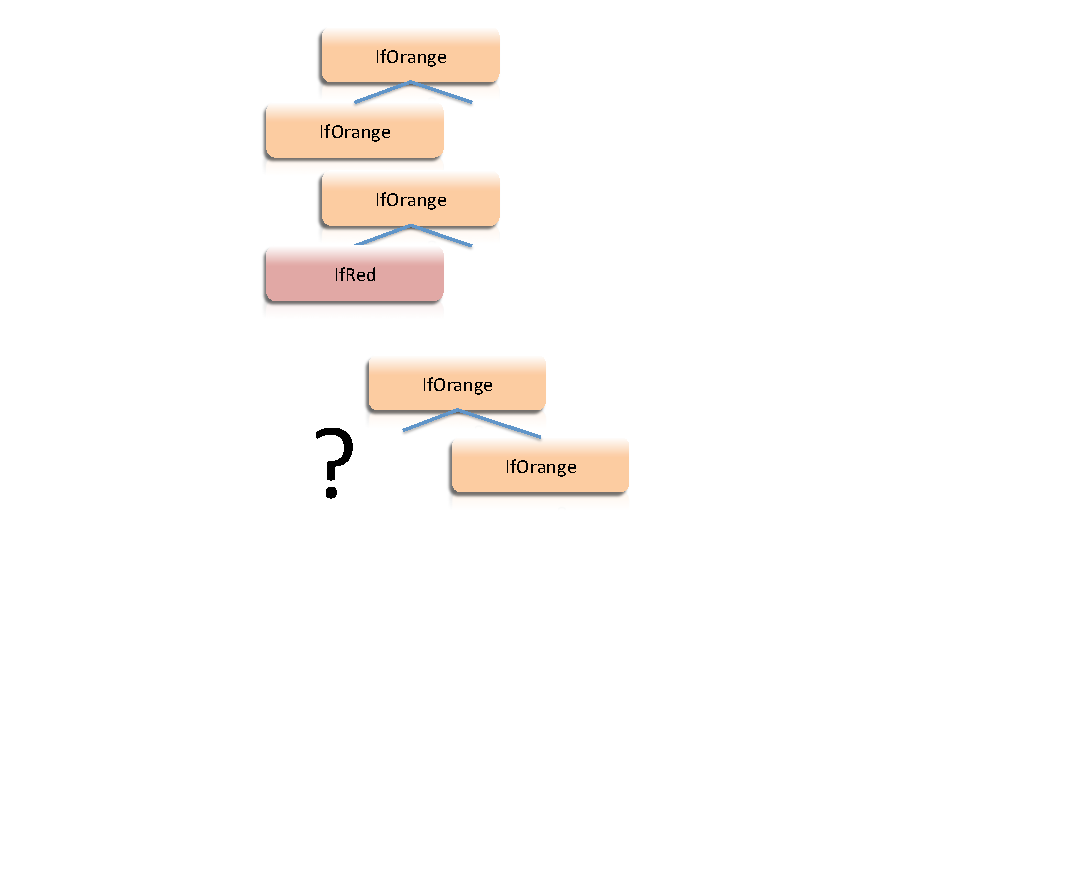
\includegraphics[width=0.45\textwidth]{figs/pdf/leng1ejem2}
\caption{Árboles válidos que carecen de sentido de la solución 1.}
\label{fig:leng1ejemplo2}
\end{figure}


\clearpage


\subsection{Solución 2: Un lenguaje de
funciones y parámetros.}\label{subsec:solucion2}

Uno de los grandes fallos de la solución 1 es que la comprobación del color de
dos casillas diferentes se convierte en un problema en si mismo. Las
comprobaciones deberían poderse hacer en una instrucción sin necesidad de generar
un árbol especifico para encontrar una casilla.

Es por ello que surge la necesidad de un lenguaje fuertemente tipado, donde
existan funciones como test que comprueban en que una casilla seleccionada por
parámetros coincida con el valor del color pasado por parámetros, es decir:
test faceUp x1 y2 colorRed(comprueba que la casilla x1 y2 de la cara de
arriba sea de color rojo). La necesidad de los parámetros se justifica porque si queremos
generar una función por cada combinación de parámetros posibles tendríamos:

\begin{equation}
   6 caras * 3 casillas_x * 3 casillas_y * 6 colores = 324 nodos
\end{equation}

Esto, además de ser un trabajo inmensamente tedioso, es difícilmente escalable y
sólo podría aplicarse al cubo de Rubik.

Por esto mismo, se crearán los distintos terminales necesarios para referirse a
las casillas (X0,X1,X2,Y0,Y1,Y2), para referirse a las caras (FaceUp, FaceFront,
FaceDown, FaceRight, FaceLeft y FaceBack) y para referirse a los colores
(ColorRed, ColorBlue, ColorGreen, ColorWhite, ColorYellow).

Adicionalmente dispondremos de una función test, que comprobará si una casilla
en concreto es de un color determinado. Si lo es, el valor devuelto de la función
será verdadero. Si no, será falso.

También tendremos todo el conjunto de operaciones condicionales como AND, OR y
NOT. La sentencia If ahora tendrá tres hijos, en lugar de dos, como pasaba en el
lenguaje anterior. El primero de los hijos representa la condición a evaluar, el
segundo es la rama del árbol que se ejecutará si la condición es cierta, si no,
se ejecutará la tercera rama del nodo.

De esta forma obtenemos conjunto de nodos terminales y no-terminales descritos
en las tablas \ref{tab:n-terminales-sol2} y \ref{tab:n-noterminales-sol2}
respectivamente (figuras \ref{fig:leng2nodosterm}, 
\ref{fig:leng2nodosnotermaction} y \ref{fig:leng2nodosnotermcond}).

\begin{table}[ctb]
\caption{Tabla de nodos terminales de la solución 2.}
\label{tab:n-terminales-sol2}
\centering
\begin{tabular}{lcp{8cm}}
\toprule
\textbf{Nombre} &\textbf{Tipo}& \textbf{Descripción}\\
\midrule
\textbf{X0}	&XNode&	Se trata de la representación de la posición x0 de una cara
del cubo de Rubik.\\\hline
\textbf{X1}	&XNode&	Se trata de la representación de la posición x1 de
una cara del cubo de Rubik.\\\hline
\textbf{X2}&	XNode&	Se trata de la representación de la
posición x2 de una cara del cubo de Rubik.\\\hline
\textbf{Y0}&	YNode&	Se trata de la
representación de la posición y0 de una cara del cubo de Rubik.\\\hline
\textbf{Y1}&YNode	&Se trata de la representación de la posición y1 de una cara
del cubo de Rubik.\\\hline
\textbf{Y2}&	YNode	&Se trata de la representación de la posición y2 de una cara
del cubo de Rubik.\\\hline
\textbf{FaceLeft}&	FaceNode	&Se trata de la representación de la cara izquierda
del cubo de Rubik.\\\hline
\textbf{FaceUp}&	FaceNode&	Se trata de la representación de la cara superior del
cubo de Rubik.\\\hline
\textbf{FaceFront}&	FaceNode &	Se trata de la representación de la cara frontal
del cubo de Rubik.\\\hline
\textbf{FaceRight}&	FaceNode&	Se trata de la representación de la cara derecha
del cubo de Rubik.\\\hline 
\textbf{FaceDown}&	FaceNode&	Se trata de la representación de la cara inferior
del cubo de Rubik.\\\hline
\textbf{FaceBack}	&FaceNode	&Se trata de la representación de la cara trasera
del cubo de Rubik.\\\hline
\textbf{Red}	&ColorNode&	Se trata de la representación del color rojo del cubo
de Rubik.\\\hline 
\textbf{Orange}&	ColorNode &	Se trata de la representación del color naranja del
cubo de Rubik.\\\hline 
\textbf{Green}	&ColorNode&	Se trata de la representación del color verde del
cubo de Rubik.\\\hline 
\textbf{White}	&ColorNode&	Se trata de la representación del color blanco del
cubo de Rubik.\\\hline 
\textbf{Yellow}&	ColorNode&	Se trata de la representación del color amarillo del
cubo de Rubik.\\\hline 
\textbf{Blue}	&ColorNode&	Se trata de la representación del color azul del cubo
de Rubik.\\\hline 
\textbf{Clockwise}&	DirectionNode&	Es el sentido de rotación de las agujas del
reloj de una cara. \\\hline 
\textbf{CounterClockwise}	&DirectionNode&	Es el sentido de rotación en sentido
contrario a las agujas del reloj de una cara.\\
\bottomrule
\end{tabular}
\end{table}

\begin{table}[ctb]
\caption{Tabla de nodos no-terminales de la solución 2.}
\label{tab:n-noterminales-sol2}
\centering
\begin{tabular}{lccp{8cm}}
\toprule
\textbf{Nombre} &\textbf{Tipo}&\textbf{Aridad}& \textbf{Descripción}\\
\midrule
\textbf{Test}	&CondNode&4&	Comprueba que en la cara especificada (nodo 0), en la
posición especificada (nodo 1 se refiere a x  y nodo 2 se refiere a  y) sea del color especificado (nodo 3).\\\hline 
\textbf{And}	&CondNode&2&Realiza la operación booleana AND entre sus dos
hijos.\\\hline
\textbf{Or}	&CondNode&2&Realiza la operación booleana OR entre sus dos
hijos.\\\hline \textbf{No}	&CondNode&1&Realiza la operación booleana NOT de su hijo.\\\hline 
\textbf{Move}	&ActionNode&2&Mueve la cara (nodo 0) en la dirección (nodo 1)
especificado.\\\hline 
\textbf{If}	&ActionNode&3&	Comprueba que la condición especificada en el hijo 0
se cumpla. Si se cumple ejecuta el subárbol del hijo 1, si no, el subárbol 2.\\\hline 
\textbf{Progn2}	&ActionNode&2&	Ejecuta todos sus hijos.\\\hline 
\textbf{Progn3}	&ActionNode&3&	Ejecuta todos sus hijos.\\
\bottomrule
\end{tabular}
\end{table}

\begin{figure}[t]
\centering
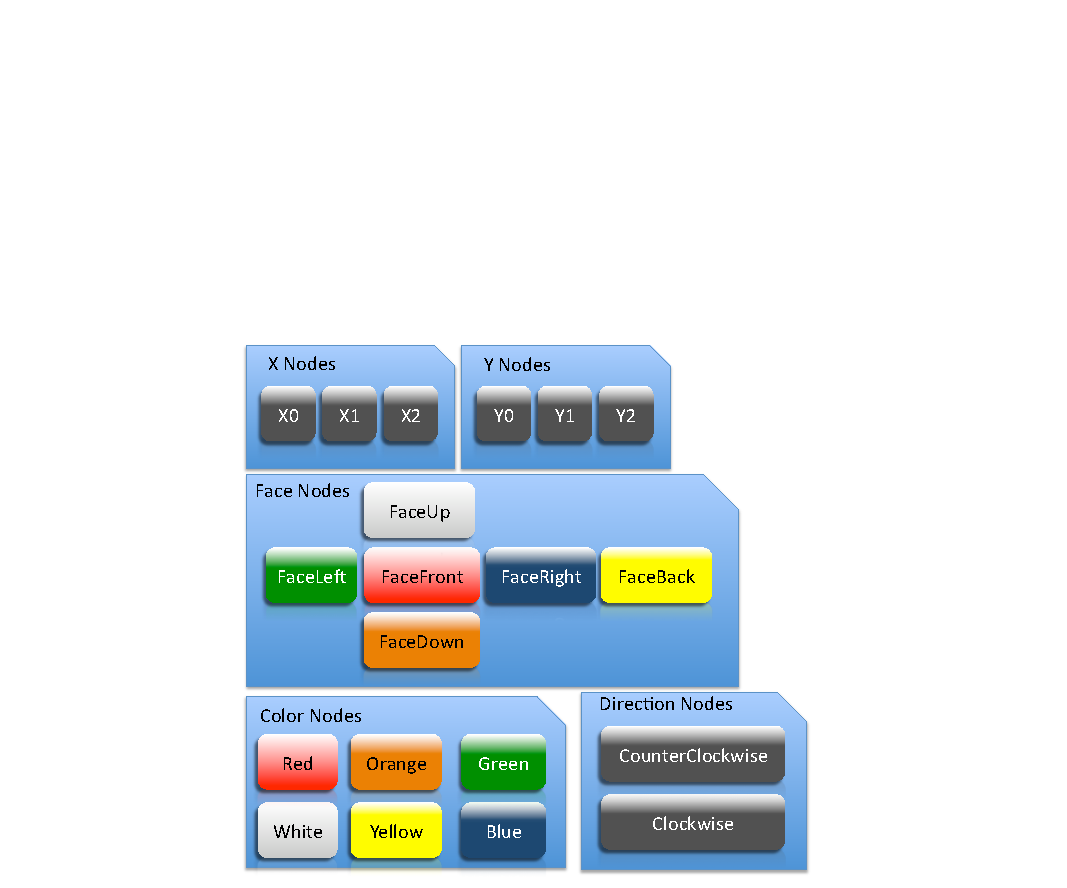
\includegraphics[width=0.65\textwidth]{figs/pdf/leng2nodosterm}
\caption{Nodos terminales de la solución 2.}
\label{fig:leng2nodosterm}
\end{figure}

\begin{figure}[t]
\centering
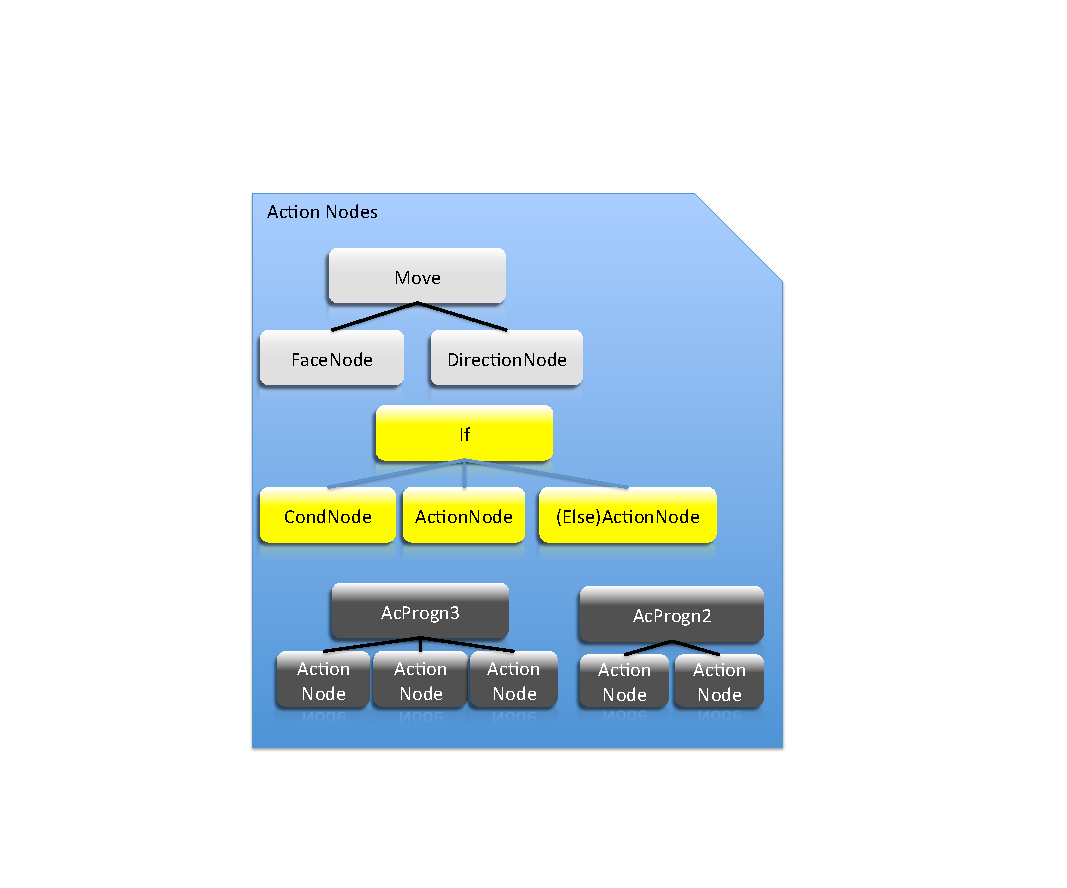
\includegraphics[width=0.65\textwidth]{figs/pdf/leng2nodosnotermaction}
\caption{Nodos no terminales de la solución 2.}
\label{fig:leng2nodosnotermaction}
\end{figure}

\begin{figure}[t]
\centering
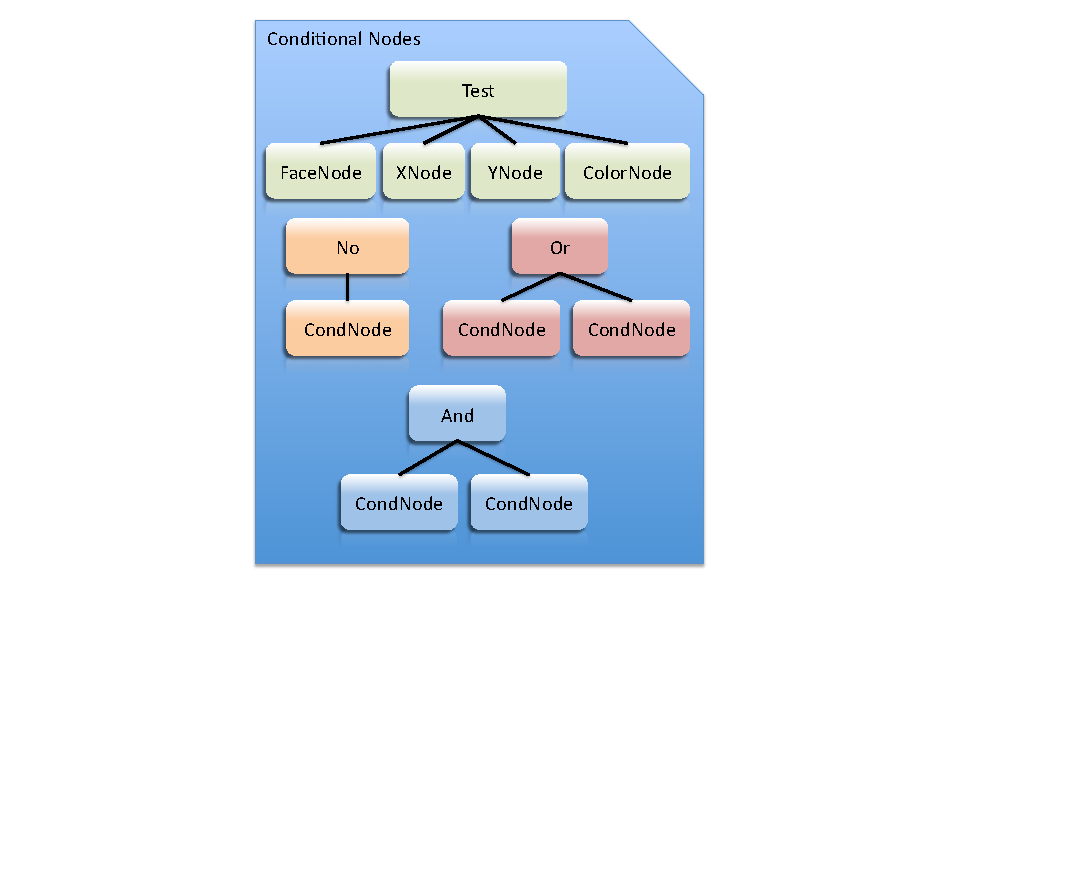
\includegraphics[width=0.65\textwidth]{figs/pdf/leng2nodosnotermcond}
\caption{Nodos no terminales de la solución 2.}
\label{fig:leng2nodosnotermcond}
\end{figure}


A diferencia con el lenguaje anterior, en este lenguaje cualquier nodo no es
compatible con otro. Por lo tanto, que la operación de cruzamiento puede que
resulte mucho más costosa y requiera de muchos más intentos para que se pueda
producir. Cuando el operador de cruzamiento ha agotado todos sus intentos de
buscar una combinación correcta del código genético, la consecuencia resultante
aparece como la copia del individuo en la nueva población. Este suceso no aporta
nada nuevo a la siguiente generación, y, por lo tanto, si no configuramos
correctamente el algoritmo, la evolución se verá comprometida.

Sin embargo, las ventajas de este lenguaje son enormes. La complejidad a la hora
de comprobar el estado del cubo ha disminuido enormemente, de tal forma que ya no
constituye un problema en si mismo. Antes, en el peor de los casos eran
necesarios nueve pasos para llegar a la casilla más distante y comprobar su
color. Ahora solo se requiere un paso. Además, las expresiones condicionales
pueden expresar situaciones mucho más complejas ya que ahora es posible utilizar
operadores como AND, OR y NO.

Para resolver el ejemplo propuesto en la solución anterior (figura
\ref{fig:leng2ejem1}) necesitaríamos de los siguientes operadores: 

\begin{algorithmic}
\IF {($Test$ $FaceUp$ $X0$ $Y0$ $Red$) $AND$ ($Test$ $FaceFront$ $X1$ $Y0$
$Red$)} 
	\STATE $Move$ $FaceLeft$ $Clockwise$
\ENDIF 
\end{algorithmic}
. Como se puede observar, la sentencia es mucho mas
simple y por otra parte, mucho más fácil de entender.

En conclusión, aunque hemos dado con un lenguaje bastante apropiado para
representar la solución del problema, necesitamos explotar la potencia de este
lenguaje. Con el árbol que hemos expuesto anteriormente sólo somos capaces de
resolver 1 caso de los 12 posibles de nivel 1 (figura \ref{fig:leng2ejem2}), lo
que resulta en unas estadísticas muy poco favorables para la complejidad del árbol. Sin duda podemos
sacar más información del árbol de programa expuesto. El siguiente lenguaje que
veremos explotará al máximo las posibilidades del este lenguaje.




\begin{figure}[t]
\centering
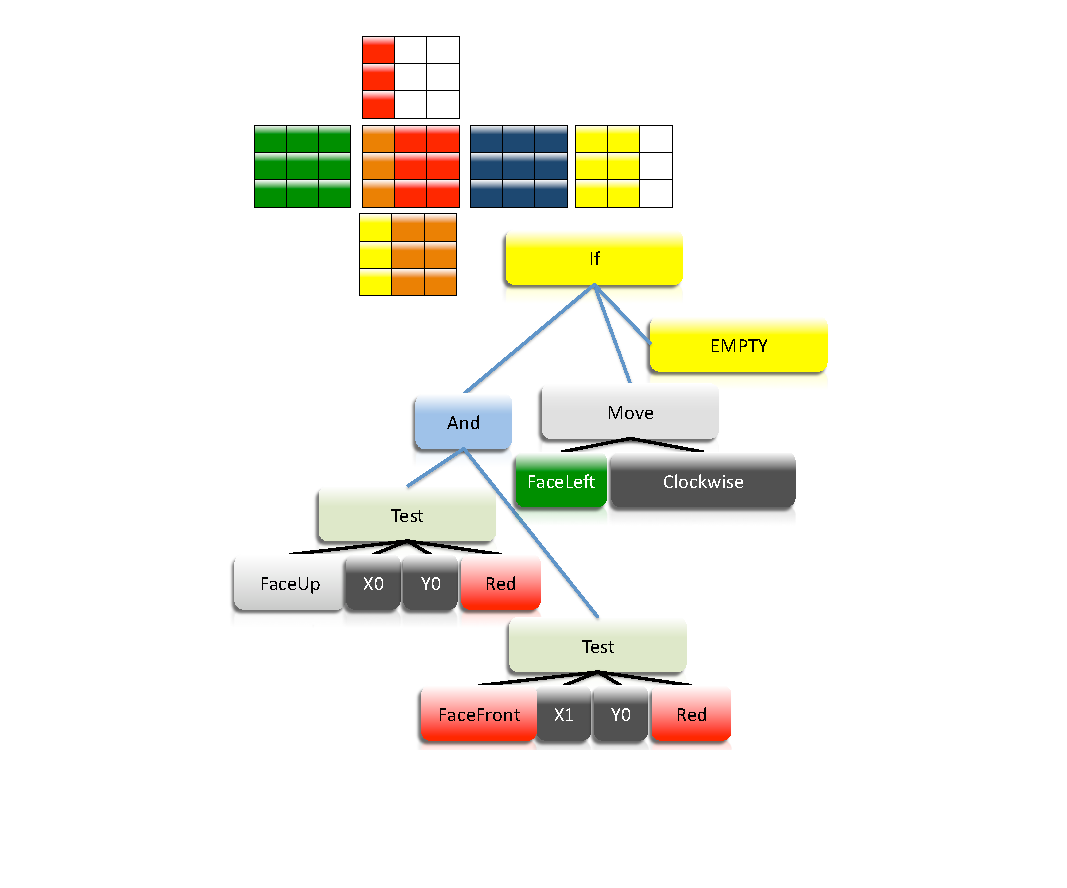
\includegraphics[width=0.65\textwidth]{figs/pdf/leng2ejem1}
\caption{Ejemplo de árbol de la solución 2 que resuelve un cubo de rubik de
nivel 1.}
\label{fig:leng2ejem1}
\end{figure}

\begin{figure}[t]
\centering
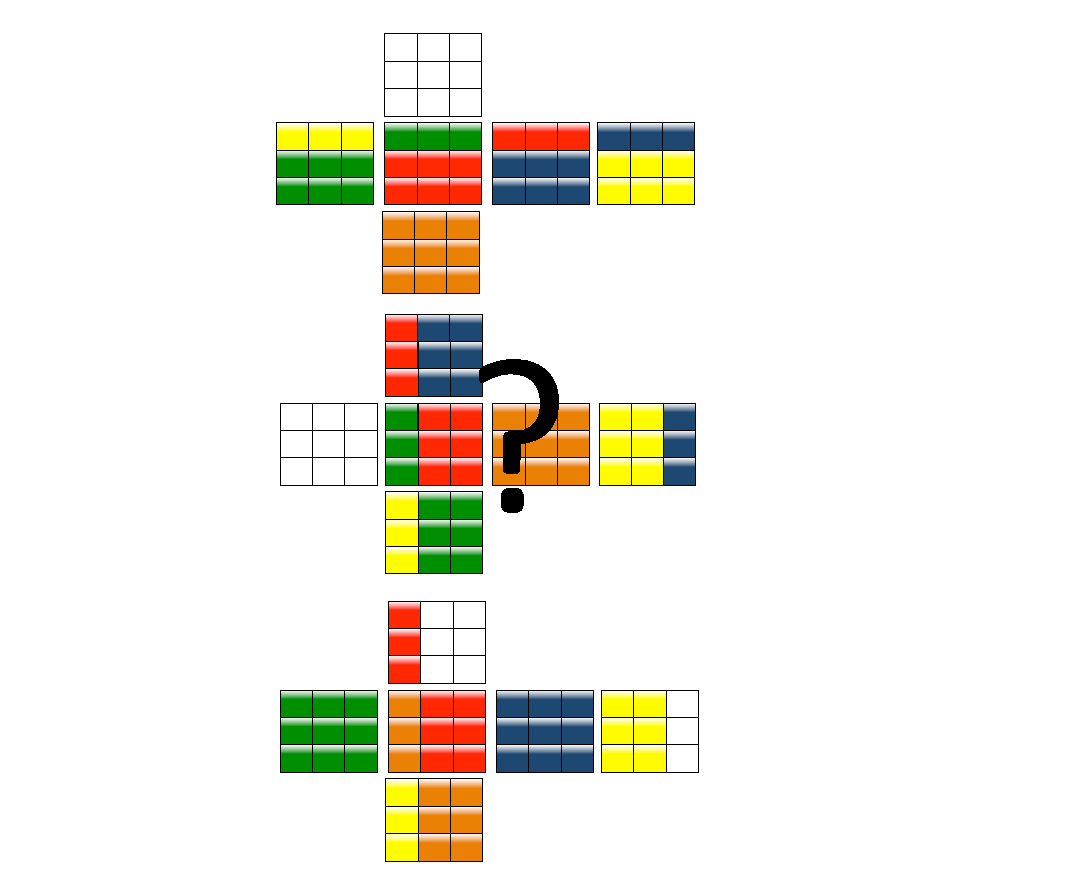
\includegraphics[width=0.45\textwidth]{figs/pdf/leng2ejem2}
\caption{Cubos de estado similar.}
\label{fig:leng2ejem2}
\end{figure}

\clearpage


\subsection{Solución 3: La abstracción del cubo.}\label{subsec:solucion3}

Una de las características del cubo de Rubik es que existen estados que son
equivalentes, simétricos: existe una serie de rotaciones del conjunto completo
que transforman un estado en otro. Nuestro cerebro es capaz de abstraer todos
estos estados y unificarlos en solo estado y por lo tanto, un camino de
resolución posible. Por otro lado, también es capaz de abstraer los colores
específicos del cubo de Rubik, y puede trabajar en la misma situación con colores
diferentes sin necesidad de adaptación alguna.

Pongamos un ejemplo. Para todos los cubos de nivel 1, es decir, con un solo
desplazamiento de la solución, nuestro cerebro solo ve dos estados diferentes y
por lo tanto dos soluciones. Estos dos casos surgen de mover cualquier cara en el
sentido de las agujas del reloj, el primero y el segundo cuando movemos una cara
en sentido opuesto a las agujas del reloj. De esta forma se podrían reducir los
12 primeros casos, en dos simples casos: cuándo debo girar en el sentido de las
agujas del reloj y cuando no.

Para imitar este comportamiento y adaptarlo a nuestro sistema se han realizado
dos modificaciones importantes sobre el segundo lenguaje.

La primera es que los colores ya no son colores concretos, como rojo o verde,
sino abstracciones como color1 o color2 que pueden tomar diferentes valores en
momentos concretos. Así en color1 puede referirse al color rojo en un momento
determinado, y luego puede referirse al verde. Una situación que no puede ocurrir
es que el color 1 se refiera al verde y el color 2 también. El color 1 es
diferente al color 2.

La segunda de estas modificaciones refleja la segunda parte del proceso de
abstracción. Para conseguirlo, el cubo será rotado en todas sus posibilidades
para cubrir todos los estados equivalentes, mientras se verifica si en alguna de
esas rotaciones se cumple la condición expuesta. Si se cumple el sistema de
rotaciones parará y dejará el cubo preparado para recibir los movimientos
pertinentes en función de la condición especificada.

Estas dos modificaciones las llevará a cabo la sentencia If y Test. If se
encargará de rotar el cubo hasta que su condición se cumpla. Si no se cumple no
se ejecutará el subárbol de acción. Además desaparece el subárbol else ya que no
tiene sentido sin un previo If que coloque el cubo en la posición adecuada.

Test se encargará de la asignación de los colores. Comprobará si existe alguna
asignación anterior al color que se quiere comprobar. Si no existe, devolverá
verdadero y asignará el color especifico al color abstracto (color 1 = red). Si
el color esta ya asignado, entonces, el color abstracto tomará ese valor. Si el
color que existe en esta posición no coincide con el color especificado, entonces
se devolverá false.

Cuando una condición no se cumple, la función If desasigna todos los colores
abstractos, rota el cubo y vuelve a empezar de nuevo, comprobando que se cumpla
la condición que anida. Una vez que se ha encontrado una forma de que la
condición se cumpla, se dejará en posición deseada el cubo de Rubik para que el
grupo de acciones que vienen a continuación actúen sobre el cubo.

Una vez planteadas las modificaciones del lenguaje se procede a describir todos 
sus nodos empezando por el grupo de terminales (tabla
\ref{tab:n-terminales-sol3}) y el grupo de terminales (tabla
\ref{tab:n-noterminales-sol3}) (figuras \ref{fig:leng3nodosterm},
\ref{fig:leng3nodosnoterma} y \ref{fig:leng3nodosnotermb}).

\begin{table}[ctb]
\caption{Tabla de nodos terminales de la solución 3.}
\label{tab:n-terminales-sol3}
\centering
\begin{tabular}{lcp{8cm}}
\toprule
\textbf{Nombre} &\textbf{Tipo}& \textbf{Descripción}\\
\midrule
\textbf{X0}&	XNode&	Se trata de la representación de la posición x0 de una cara
del cubo de Rubik.\\\hline
\textbf{X1}&	XNode&	Se trata de la representación de la posición x1 de
una cara del cubo de Rubik.\\\hline
\textbf{X2}&	XNode&	Se trata de la representación de
la posición x2 de una cara del cubo de Rubik.\\\hline
\textbf{Y0}&	YNode&	Se trata de la
representación de la posición y0 de una cara del cubo de Rubik.\\\hline
\textbf{Y1}& YNode&	Se trata de la representación de la posición y1 de una cara
del cubo de Rubik. \\\hline
\textbf{Y2}&	YNode&	Se trata de la representación de la posición y2 de
una cara del cubo de Rubik. \\\hline
\textbf{FaceLeft}&	FaceNode&	Se trata de la
representación de la cara izquierda del cubo de Rubik.\\\hline
\textbf{FaceUp}&	FaceNode&
Se trata de la representación de la cara superior del cubo de Rubik.\\\hline
\textbf{FaceFront}&	FaceNode &	Se trata de la representación de la cara frontal
del cubo de Rubik.\\\hline
\textbf{FaceRight}&	FaceNode&	Se trata de la representación de la cara derecha
del cubo de Rubik.\\\hline
\textbf{FaceDown}&	FaceNode&	Se trata de la representación de la cara inferior
del cubo de Rubik.\\\hline
\textbf{FaceBack}&	FaceNode&	Se trata de la representación de la cara trasera
del cubo de Rubik.\\\hline
\textbf{Color1}&	ColorNode	&Se trata de la abstracción de un color del cubo de
Rubik.\\\hline
\textbf{Color2}&	ColorNode &	Se trata de la abstracción de un color del cubo de
Rubik.\\\hline
\textbf{Color3}&	ColorNode&	Se trata de la abstracción de un color del cubo de
Rubik.\\\hline
\textbf{Color4}&	ColorNode&	Se trata de la abstracción de un color del cubo de
Rubik. \\\hline
\textbf{Color5}&	ColorNode&	Se trata de la abstracción de un color del cubo de
Rubik.\\\hline
\textbf{Color6}&	ColorNode&	Se trata de la abstracción de un color del
cubo de Rubik.\\\hline
\textbf{Clockwise}&	DirectionNode&	Es el sentido de rotación de
las agujas del reloj de una cara.\\\hline
\textbf{CounterClockwise}&	DirectionNode&	Es el
sentido de rotación en sentido contrario a las agujas del reloj de una
cara.\\
\bottomrule
\end{tabular}
\end{table}

\begin{table}[ctb]
\caption{Tabla de nodos no-terminales de la solución 3.}
\label{tab:n-noterminales-sol3}
\centering
\begin{tabular}{lccp{8cm}}
\toprule
\textbf{Nombre} &\textbf{Tipo}&\textbf{Aridad}& \textbf{Descripción}\\
\midrule
\textbf{Test}&CondNode&	4	&Comprueba que en la cara especificada (nodo 0), en la
posición especificada (nodo 1 se refiere a x  y nodo 2 se refiere a  y) sea del
color especificado (nodo 3).\\\hline
\textbf{And}&	CondNode&	2&	Realiza la operación booleanas AND entre sus dos
hijos.\\\hline 
\textbf{Or}&	CondNode&	2&	Realiza la operación booleana OR entre sus
dos hijos.\\\hline
\textbf{No}& CondNode&	1&	Realiza la operación booleana NOT de su
hijo.\\\hline
\textbf{If}&IfNode&	2&	Se
trata de la representación de la posición y2 de una cara del cubo de
Rubik.\\\hline
\textbf{Progn2}&	IfNode	&2&	Ejecuta todos sus hijos.\\\hline
\textbf{Progn3}&	IfNode	&3&	Ejecuta todos sus hijos.\\\hline
\textbf{Move}	&ActionNode	&2&	Mueve la cara (nodo 0) en la dirección (nodo 1)
especificado.\\\hline
\textbf{Progn2}&	ActionNode	&2&	Ejecuta todos sus hijos.\\\hline
\textbf{Progn3}&	ActionNode	&3&	Ejecuta todos sus hijos.\\
\bottomrule
\end{tabular}
\end{table}

\begin{figure}[ctb]
\centering
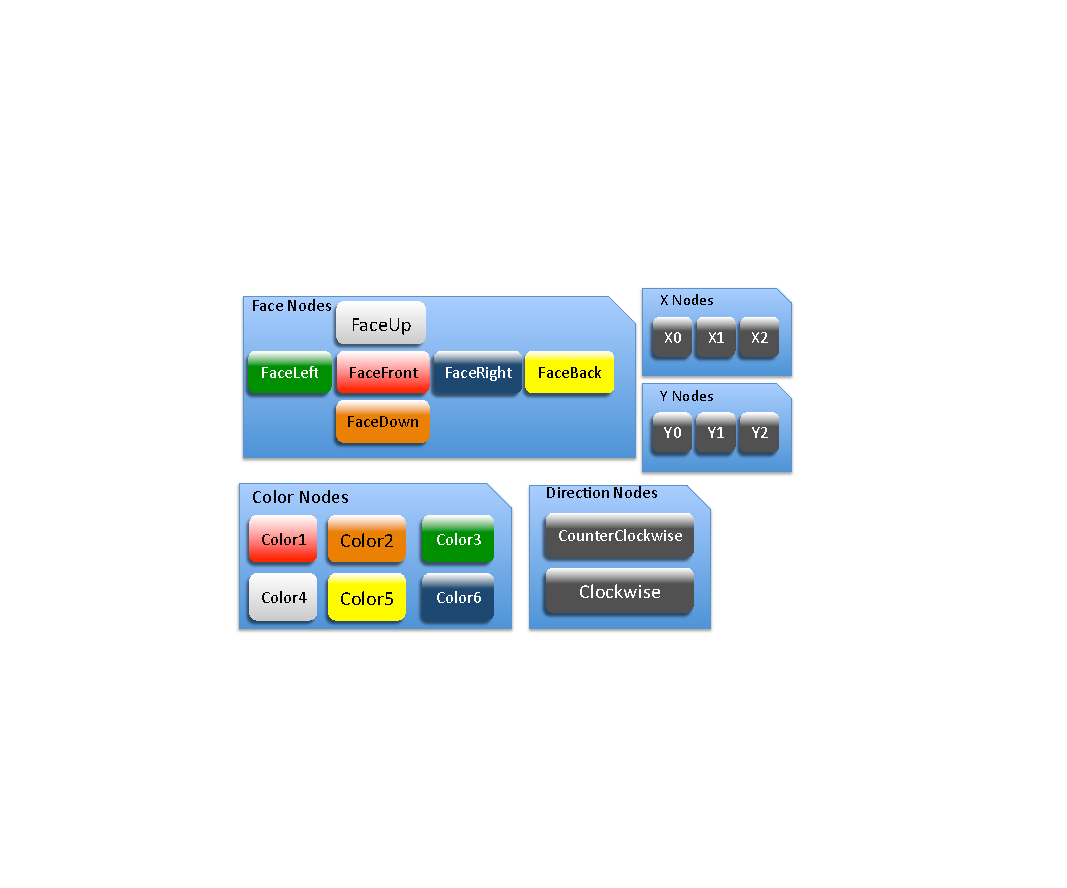
\includegraphics[width=0.65\textwidth]{figs/pdf/leng3nodosterm}
\caption{Nodos terminales de la solución 3.}
\label{fig:leng3nodosterm}
\end{figure}

\begin{figure}[ctb]
\centering
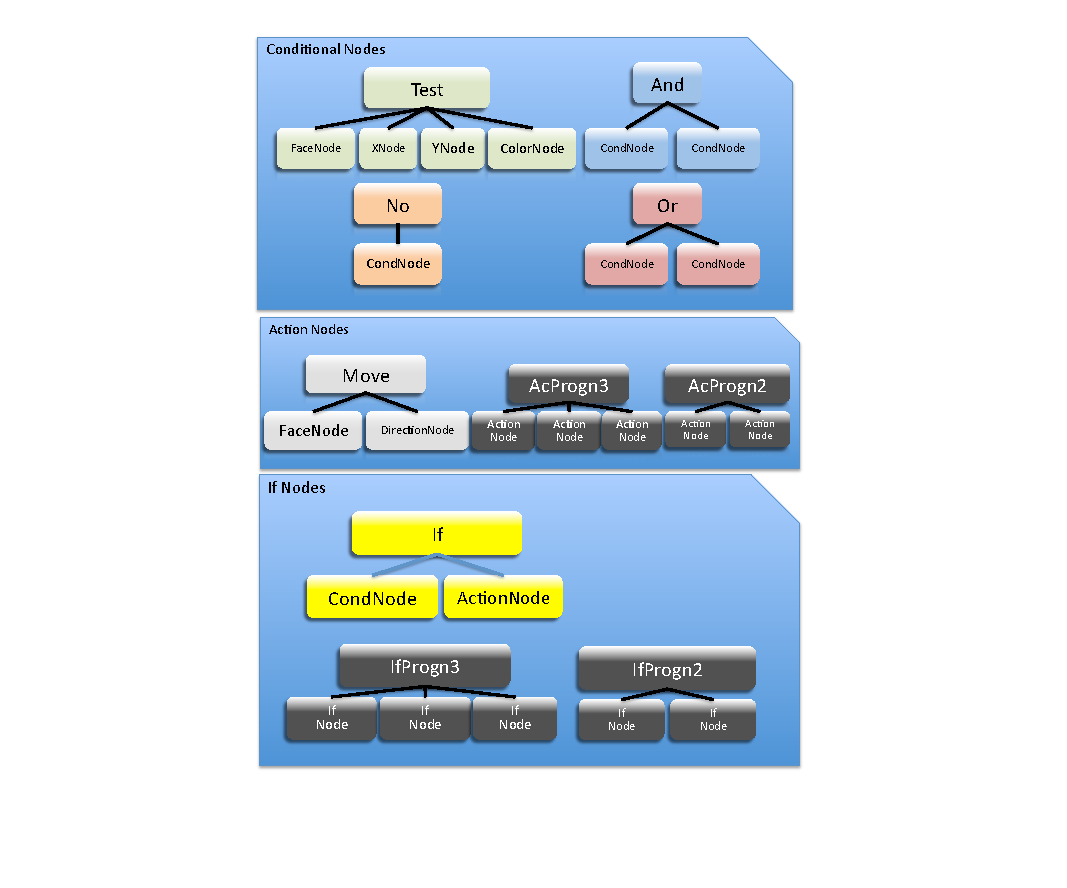
\includegraphics[width=0.65\textwidth]{figs/pdf/leng3nodosnoterma}
\caption{Nodos no terminales de la solución 3.}
\label{fig:leng3nodosnoterma}
\end{figure}

\begin{figure}[ctb]
\centering
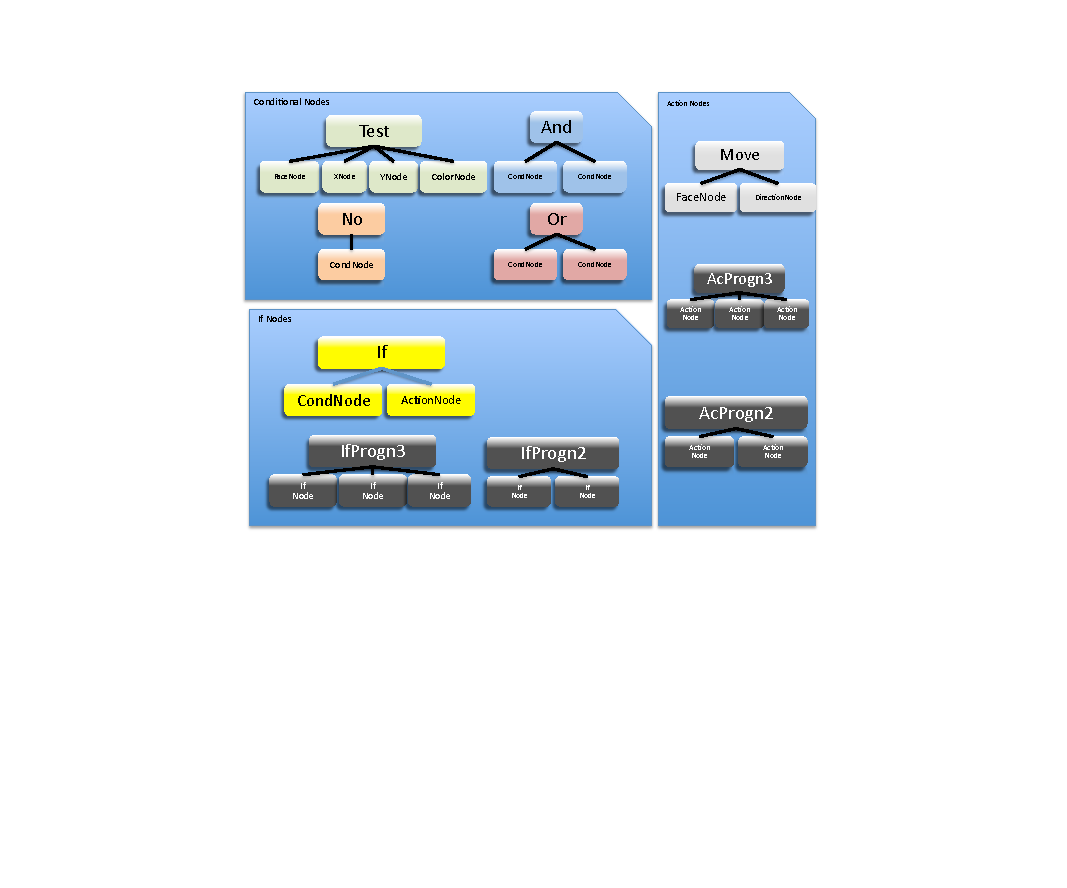
\includegraphics[width=0.65\textwidth]{figs/pdf/leng3nodosnotermb}
\caption{Nodos no terminales de la solución 3.}
\label{fig:leng3nodosnotermb}
\end{figure}

Este lenguaje presenta los mismo síntomas y problemas que aparecían en el 
anterior con la diferencia de que el nodo If no contiene Else. Además, la
anidación de sentencias If deja de tener sentido por lo que nuestro programa
pasará a ser una “lista” de sentencias If ya que los operadores de movimiento no
tienen sentido si no existen un If que lo contenga.

Las ventajas son claras y evidentes. Donde antes resolvíamos dos cubos de Rubik,
ahora resolvemos doce (figuras \ref{fig:leng3ejem1} y \ref{fig:leng3ejem2}). Es
decir, nuestro lenguaje resulta mucho más potente. Otro factor a tener en cuenta es que al ser un lenguaje altamente tipado el bloat que
se puede producir es menor.




\begin{figure}[t]
\centering
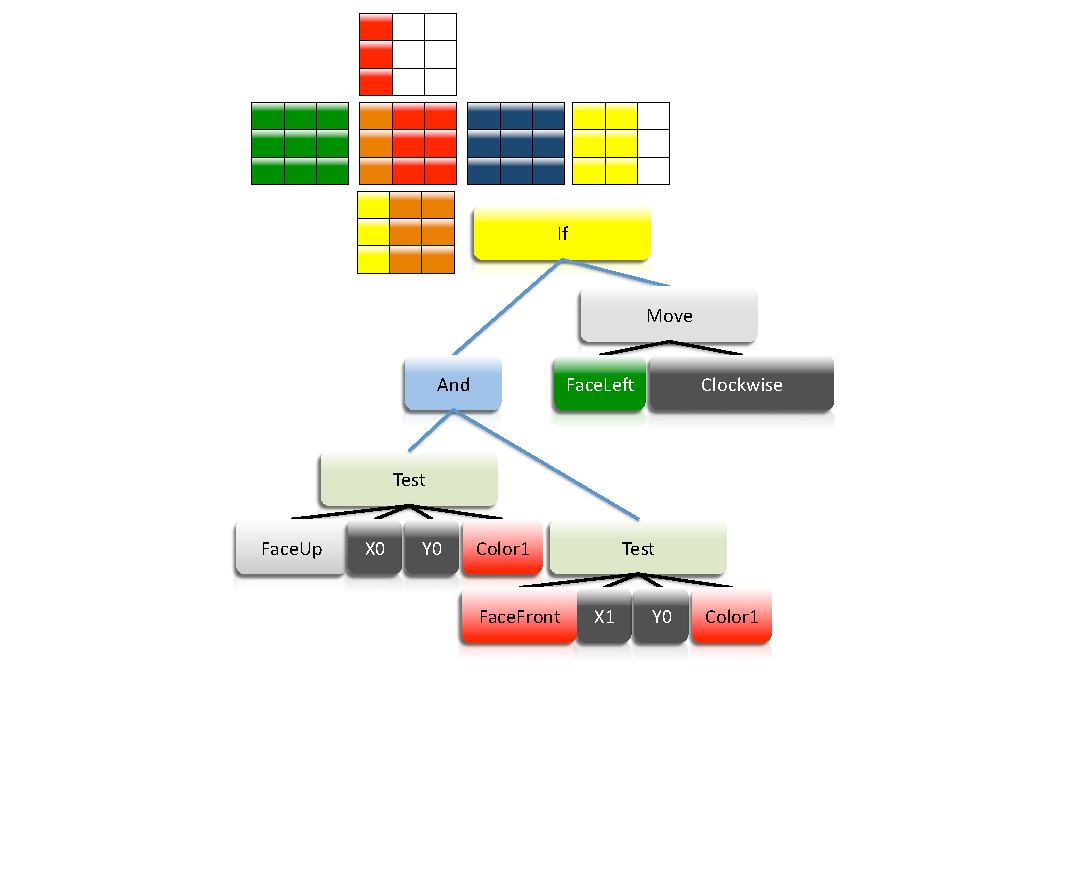
\includegraphics[width=0.65\textwidth]{figs/pdf/leng3ejem1}
\caption{Ejemplo de árbol de la solución 3 que resuelve un cubo de rubik de nivel 1.}
\label{fig:leng3ejem1}
\end{figure}

\begin{figure}[t]
\centering
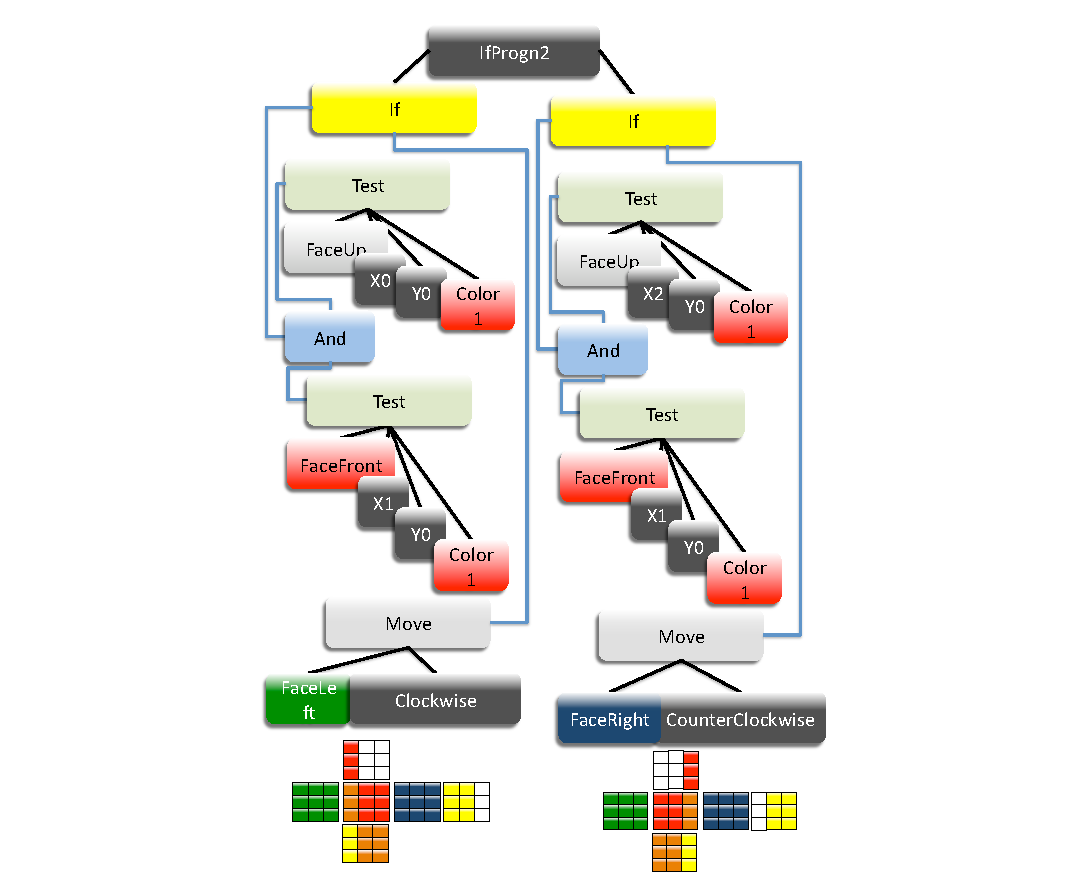
\includegraphics[width=0.9\textwidth]{figs/pdf/leng3ejem2}
\caption{Árbol que resuelve todos los cubos de rubik de nivel 1.}
\label{fig:leng3ejem2}
\end{figure}

\clearpage

\section{Fitness}\label{sec:fitness}


El fitness es una nota o un conjunto de calificaciones o notas de un programa que
sirven para decidir cuando un programa es mejor que otro. En nuestro caso
necesitamos varias medidas de fitness. Necesitamos un valor que nos indique lo
cerca de la solución que un programa deja a los cubos. De esta forma, un programa
será mejor cuanto más cerca de la solución deje el cubo. A esta puntuación se la
llamará entropía, descrita en el siguiente punto.

No obstante, cuando tenemos varios cubos en juego podemos obtener más información
sobre el rendimiento del algoritmo. Por ejemplo podremos saber cuántos cubos
resuelve un programa. Es más, ya que tenemos una manera de clasificar los cubos
mediante sus dificultades, podemos sesgar la búsqueda y guiar a los programas
para que primen los cubos difíciles respecto a los más fáciles.

Otro dato que necesitamos saber es la longitud de las soluciones. Ya que nos
conviene encontrar el camino óptimo, necesitamos saber el tamaño de la solución
para poder elegir el programa que menor longitud de solución tenga.

Por último, para controlar el bloat producido, podremos considerar en el fitness
el número de nodos que posee el programa, ya que si encontramos un programa que
hace lo mismo con menos código puede sernos de interés.

Al final del proceso, cuando estamos comparando dos programas, uno tiene que
inclinarse a por elegir uno u otro. Para ello necesitaremos comparar y unir de
alguna forma todos estos objetivos en un objetivo común. De esto hablaremos en el
último punto de este apartado. 

\subsection{Entropía}\label{subsec:entropia}

La razón de esta medición es que nos interesa saber cuánto de cerca estamos de
solventar el cubo de Rubik. Podríamos obtener este dato mediante la utilización
de algoritmos de resolución del cubo de Rubik existentes. No obstante, estos
algoritmos utilizan muchos recursos y multiplicando éstos por cada individuo de
la población resultaría una utilización inviable de los recursos y la potencia de
cálculo del sistema. Por otro lado necesitamos un criterio ajeno a cualquier
sistema de búsqueda preexistente para no predeterminar a los individuos. Por lo
tanto hemos desarrollado un método basado en la entropía del cubo que nos dirá
con más o menos acierto lo cerca que estamos de una solución.

\begin{figure}[t]
\centering
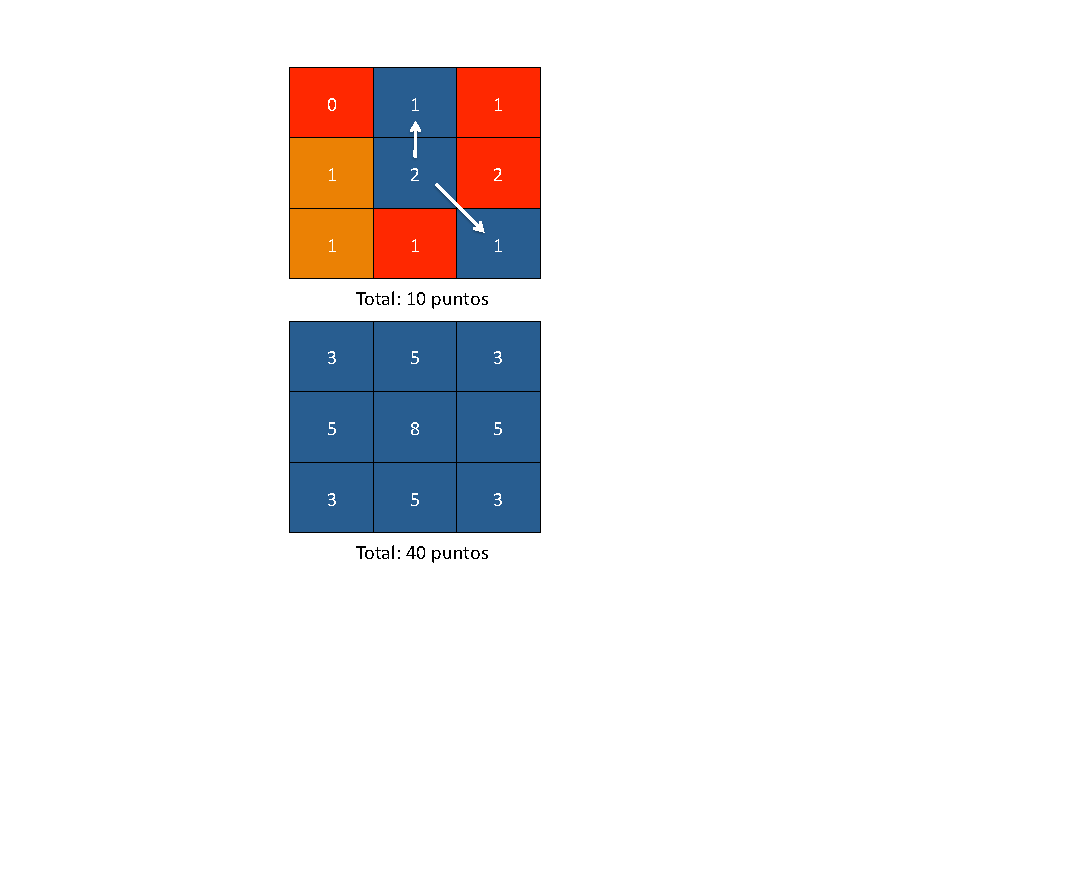
\includegraphics[width=0.35\textwidth]{figs/pdf/entropia}
\caption{Entropía.}
\label{fig:entropia}
\end{figure}

El cálculo de la entropía del cubo consiste en la suma de las casillas del mismo
color que estén contiguas dentro de una misma cara. Es decir, sumamos un punto
por cada casilla que esté contigua dentro de la misma cara y que sea del mismo
color. Por consiguiente, una cara resuelta sumaría 40 puntos
(figura \ref{fig:entropia}), y entonces un cubo de Rubik resuelto sumaría 240
puntos.

El pseudocódigo del algoritmo sería el siguiente:


\begin{algorithmic}
\FOR{each cara}
	\STATE puntuacionCara = $0$
	\FOR{each casilla}
		\IF {CasillaArriba.color == CasillaActual.color}  
				\STATE puntuacionCara++
		\ENDIF
		\IF {CasillaArribaIzq.color == CasillaActual.color}  
				\STATE puntuacionCara++
		\ENDIF
		\IF {CasillaIzquierda.color == CasillaActual.color}  
				\STATE puntuacionCara++
		\ENDIF
		\IF {CasillaAbajoIzq.color == CasillaActual.color}  
				\STATE puntuacionCara++
		\ENDIF
		\IF {CasillaAbajo.color == CasillaActual.color}  
				\STATE puntuacionCara++
		\ENDIF
		\IF {CasillaAbajoDer.color == CasillaActual.color}  
				\STATE puntuacionCara++
		\ENDIF
		\IF {CasillaDerecha.color == CasillaActual.color}  
				\STATE puntuacionCara++
		\ENDIF
		\IF {CasillaArribaDer.color == CasillaActual.color}  
				\STATE puntuacionCara++
		\ENDIF
	\ENDFOR 
	\STATE puntuacionTotal += puntuacionCara
\ENDFOR 
\end{algorithmic}

Con este método es posible encontrar estados intermedios más cercanos a la meta
que posean menor entropía. Sin embargo, la tendencia general del cubo es a
aumentar el orden de las casillas según se acerque a la solución. Además, esta
medida se utilizará para comparar el estado final del cubo finalizada la
ejecución de un programa frente al estado final del mismo cubo finalizada la
ejecución de otro programa, por lo tanto, esta nota no servirá para evaluar
estados intermedios sino sólo los finales.
 
\subsection{Cubos resueltos}\label{subsec:cubosresueltos}

Una vez que conseguimos resolver cubos, es trivial comparar programas en función
del número de cubo que resuelve uno y el número de cubos de Rubik que resuelve
otro. Sin embargo, podemos explotar esta medición incorporando nuevos parámetros,
como es la dificultad de los cubos resueltos.

Al generar los primeros programas podemos ver en las estadísticas que existen muy
pocos de ellos que puedan resolver un cubo de alta dificultad. Sin embargo, de
los programas generados por el algoritmo genético hay muchos más que pueden
resolver cubos fáciles. Y esos programas que resuelven cubos fáciles son, además,
capaces de resolver muchas clases de cubos fáciles. Por el contrario, los
programas resolvedores de cubos difíciles sólo son capaces de resolver un número
muy limitado de dichos cubos.

Como el algoritmo selecciona los programas que más cubos resuelven, los
resolvedores de cubos difíciles van desapareciendo, de tal forma que sólo
sobreviven los programas capaces de resolver los cubos fáciles. Esto hace que
disminuya enormemente la diversidad genética de nuestro sistema. En definitiva
necesitamos buscar alguna forma de calibrar el fitness para mantener con vida a
los individuos que pueden resolver cubos difíciles.

Así, necesitamos premiar de alguna forma a los programas que resuelven cubos
difíciles. Una alternativa sería realizar una suma ponderada linealmente de los
cubos resueltos de cada dificultad. Sin embargo la ponderación lineal no pondera
lo suficiente ya que, es fácil encontrar un programa que resuelva más cubos de
dificultad fácil que de la dificultad estrictamente superior. Esto es debido a
que por cada nivel aparecen doce nuevas posibilidades, por lo que, resolver el
siguiente nivel resulta doce veces más difícil. Es por esto que necesitamos una
ponderación exponencial.

Sin embargo en la ponderación necesitamos encontrar un factor que regule la suma
de los cubos resueltos de diferentes niveles. La forma de encontrar este valor
será de forma empírica, buscando el valor que obtenga el mejor rendimiento de la
evolución. Para ello la base de la potencia será configurable mediante parámetros
del algoritmo.

La fórmula
\begin{equation}
   p = c*f ^ d,
\end{equation}
es la fórmula del fitness donde $p$ es la puntuación del programa, $c$ son los
cubos resueltos por el programa, $f$ es el factor elegido y $d$ es la
dificultad de los cubos resueltos.
 

La puntuación final del programa será la suma de las multiplicaciones del número
de cubos resueltos de una dificultad por un factor elevado a la dificultad del
cubo resuelto.


\subsection{Longitud de la solución}\label{subsec:long-solucion}


Para poder controlar la longitud de las soluciones de los cubos que genera un
programa es necesario tener en cuenta este hecho en el fitness. Calcular las
longitudes de las soluciones de los programas es un proceso muy sencillo. Lo
único que requiere es un contador que se inicializa a cero antes de intentar
resolver cualquier cubo de Rubik. Posteriormente, en cada ocasión que se rota una
cara de un cubo se sumará una unidad a este contador. Una vez que la ejecución
del árbol de programa ha terminado, es decir, el programa ha terminado de
intentar resolver el cubo en cuestión, se guardará el número de pasos realizados
por el programa para este cubo. Este proceso se repetirá por cada cubo de Rubik a
resolver.

Cuando el programa termine de intentar resolver todos los cubos de Rubik que le
han sido asignados en el proceso de evaluación, se calculará la media del número
de pasos alcanzado en cada cubo. En base a esa media podremos determinar que
programa es capaz de generar soluciones generalmente más cortas.

\subsection{Bloat}\label{subsec:bloat}

El bloat es el código que se genera dentro los programas evolucionados que carece
de sentido. Como la evolución es un proceso aleatorio, no se encarga de verificar
si el código que se genera tiene sentido o no tiene sentido. Es por ello que
tenemos que realizar esta comprobación de forma manual. Para ello lo único que
tenemos que hacer es calcular el número de nodos que hay en nuestro sistema. Esto
se hace utilizando un simple algoritmo recursivo que recorre todos los nodos del
árbol del programa, contando uno por cada nodo que pasa.

Una vez que tenemos esta función, podremos decir que un programa será mejor
cuando tenga menos nodos que otro programa, es decir, contenga menos
instrucciones.

\subsection{Combinación del fitness}\label{subsec:combinacion-fitness}

Una vez que tenemos preparados numéricamente todos los objetivos necesitaremos
crear un criterio de unión para fusionar todas las calificaciones de un programa.
Como hemos visto en el apartado del estado del arte, existen multitud de maneras
de combinar todos estos objetivos. Nosotros hemos escogido utilizar una política
de prioridades, es decir, definimos la existencia de calificaciones que
prevalecen sobre otras, y sólo cuando las calificaciones de nivel superior son
iguales en ambos programas, el resto de calificaciones serán estudiadas en mas
detalle.

Hemos optado por esta política ya que hemos comprobado que el hacer un control
del bloat demasiado exhaustivo durante la propia evolución puede impedir que ella
misma tenga lugar, por lo que para no tener problemas, sólo se utilizará cuando
consigamos resolver todos los cubos de Rubik.

El mismo efecto que el bloat tiene el número de pasos. Como es obvio, no mover
nada en el cubo de Rubik tiene menos pasos que mover algo. Como nuestro primer
objetivo es conseguir resolver todos los cubos de Rubik, necesitamos que el
sistema mueva las caras. Por lo tanto, esta calificación tampoco se tendrá en
cuenta hasta que se hayan resuelto todos los cubos propuestos en la evaluación.

La entropía nos valdrá para deqcidir qué programa es mejor que otro cuando exista
un empate numérico de la puntuación de cubos resueltos. Esto se justifica en que
cuando dos programas consiguen resolver el mismo número de cubos, el programa que
mas se acerque a la solución, más cerca estará de resolver un cubo de Rubik y por
lo tanto, de mejorar la puntuación de cubos resueltos.

Como adelantaba, la puntuación principal será la de los cubos resueltos expuesta
en la sección \ref{subsec:cubosresueltos}. Esto es debido a que el objetivo
principal es resolver los cubos, y este índice nos muestra directamente el número de cubos que es capaz de
resolver un programa.

Resumiendo, la formula de fitness será la siguiente:

%Si (yo.cubosResueltos > otro.cubosResueltos)	
%Entonces yo_gano; 
%Si (yo.cubosResueltos < otro.cubosResueltos)	
%Entonces otro_gana;
%Si (yo.entropia > otro.entropia)
%Entonces yo_gano;
%Si (yo.entropia < otro.entropia)
%Entonces otro_gana;
%Si (TodoResuelto) Entonces
%	Si (yo.pasos < otro.pasos)
% 		Entonces yo_gano
% 	Si (yo.pasos > otro.pasos)
% 		Entonces otro_gana
%	Si (yo.tamaño < otro.tamaño)
%		Entonces yo_gano
%Si (yo.tamaño > otro.tamaño)
%		Entonces otro_gana
%
%Si no ha ganado nadie se elige uno aleatoriamente.

\begin{algorithmic}

		\IF {yo.cubosResueltos $>$ otro.cubosResueltos}  
				\RETURN yogano
		\ENDIF
		
		\IF {yo.cubosResueltos $<$ otro.cubosResueltos}  
				\RETURN otrogana
		\ENDIF
		\IF {yo.entropia $>$ otro.entropia}  
				\RETURN yogano
		\ENDIF
		\IF {yo.entropia $<$ otro.entropia}  
				\RETURN otrogana
		\ENDIF
		\IF {TodoResuelto}  
			\IF {yo.pasos $<$ otro.pasos}  
					\RETURN yogano
			\ENDIF
			\IF {yo.pasos $>$ otro.pasos}  
					\RETURN otrogana
			\ENDIF
			\IF {yo.tamaño $<$ otro.tamaño}  
					\RETURN yogano
			\ENDIF
			\IF {yo.tamaño $>$ otro.tamaño}  
					\RETURN otrogana
			\ENDIF
		\ELSE 
			\RETURN random 
			\COMMENT{Si no ha ganado nadie se elige uno aleatoriamente}
			
		\ENDIF
\end{algorithmic}



\section{Evaluación}\label{sec:evaluacion}

El proceso de evaluación consiste en enfrentar a los programas contra una batería
de pruebas suficientes para poder calcular un fitness que consiga representar
precisamente las cualidades del programa y en función de esas cualidades elegir a
los individuos más aptos.

Al inicio del proyecto se empezó a probar los programas con un cubo diferente por
cada evaluación y programa (especial atención a este hecho). Esto tenía como
consecuencia que a los programas con “suerte” les tocaba un cubo más fácil o que
supieran resolver de antemano y, con esta clara ventaja, se situaban como lideres
de la población. Sin embargo, en la siguiente generación, el cubo con el que
tenían que enfrentarse era diferente y por lo tanto, es probable que no supieran
resolverlo. Es por esto que el sistema divagaba entre individuos y no mostraba
una tendencia clara de evolución. Este método de trabajo no resulta apropiado
para explotar la potencia del sistema.

Al sistema anterior le llamaremos evaluación dinámica, donde cada evaluación es
diferente. Al ser diferente depende de factores aleatorios y puede favorecer a
ciertos individuos que en realidad no contienen la información que nos interesa
explotar. Las pruebas a las que sometemos a la población pueden no ser del mismo
grado de dificultad y por lo tanto hay ciertos individuos que saldrían muy
aventajados de este hecho.

Además, generar un cubo en cada evaluación resulta muy costoso y por otro lado
resulta muy complicado optimizar dicho proceso. Esto es debido a que al ser una
evaluación dinámica, no se pueden guardar los resultados de cada una de ellas
para posteriores evaluaciones. Por lo tanto este sistema de evaluación consume
demasiados recursos aportando resultados muy pobres.

Posteriormente, decidimos cambiar este método de evaluación y someter a la
población siempre a las mismas pruebas. El problema ahora es garantizar que el
mejor programa sea capaz de resolver cubos que no existen en la muestra. Éste es
el típico problema de la IA, donde se prepara un conjunto de entrenamiento y un
conjunto de pruebas, diferente al de entrenamiento, para verificar que nuestros
individuos no aprenden solamente los cubos presentados en el conjunto de
entrenamiento.

Sin embargo, el sistema evolutivo es lo suficientemente pesado sólo con el
conjunto de entrenamiento como para, además, realizar otra evaluación con otro
conjunto diferente. Es por esto que se probarán los programas simplemente con el
conjunto de entrenamiento y, al final del proceso, se verificará las cualidades
de abstracción del individuo resultante.

Así, el conjunto de cubos de entrenamiento tiene que ser lo suficientemente
grande como para que podamos extrapolar los resultados a todas las posibilidades
de cubos de Rubik existentes. Por lo tanto, intentaremos probar con el mayor
número de cubos posibles para que las pruebas sean viables.

Hay que tener en cuenta que otra ventaja importante es que al ser siempre el
mismo conjunto de entrenamiento, no necesitamos reevaluar a los individuos, ni
generar nuevos cubos en cada evaluación y por lo tanto, el sistema puede probar
muchos más cubos en el mismo tiempo.

En concreto, en el concurso para el que el sistema fue diseñado, especificaban
que en sus pruebas utilizarían 1000 cubos diferentes para evaluar el rendimiento
del programa. Es por esto que, para garantizar que nuestro programa resuelve al
menos 1000 cubos, se probará con al menos 2000 cubos diferentes.

Este sistema de evaluación estática facilitó enormemente la toma de decisiones.
Las puntuaciones se mantenían constantes y se percibía perfectamente cuando se
producía una mejora en la población.

El conjunto de entrenamiento como hemos dicho, tiene que contener una muestra
suficiente de cubos para que podamos afirmar que hemos creado un resolvedor. Para
crear el conjunto de entrenamiento, hablaremos primero de cómo hemos clasificado
a los cubos de Rubik dentro de diferentes dificultades.  La dificultad de un
determinado cubo de Rubik son los pasos mínimos que se han realizado para llegar
a ese estado.

Existen dos formas de generar los cubos. La forma número uno, generará todas las
posibilidades existentes de esa dificultad. Es decir, existirán 12 posibilidades
de dificultad 1, ya que existen 12 movimientos posibles en el cubo de Rubik. De
dificultad 2 existirán 144 posibilidades, aunque estas posibilidades incluyen
cubos resueltos y repetidos.

La segunda forma de generar cubos se utilizará cuando no podamos almacenar todos
los cubos posibles. De esta manera, en la muestra generada, querremos tener una
muestra representativa del nivel de dificultad, sin que existan cubos repetidos y
además que estos pertenezcan al nivel de dificultad adecuado. Para conseguir
cubos de la dificultad especificada vamos a utilizar la medida de entropía para
generar los cubos. El método consiste en mover aleatoriamente una cara en un
sentido aleatorio siempre que la entropía del cubo sea menor (más desordenado)
tantas veces como el nivel de dificultad requiera. Si llegado un número
determinado de intentos, no se consigue alcanzar una entropía menor, se empezará
a mover el cubo de forma aleatoria hasta que, en algún estado, la entropía del
cubo sea menor. De esta forma nos aseguramos que un cubo de nivel 3 tenga por lo
menos nivel 3.

Una vez que sabemos como se generan los cubos, hemos comprobado que a partir de
la dificultad 10, la máquina virtual de Java suele dar problemas de memoria a la
hora de generar cubos, por lo que creemos que un cubo de dificultad 10 es un cubo
verdaderamente desordenado. Como queremos resolver al menos 2.000 cubos,
necesitamos que los programas se vayan enfrentando a todas las dificultades desde
un principio, y a medida que evolucionen, las dificultades más fáciles se
resolverán completamente.

Por lo tanto los 2.000 cubos planteados se distribuirán equitativamente por todas
las dificultades, de esta forma, si tenemos 10 dificultades, generaremos 200
cubos por dificultad. Por supuesto, de nivel 1 y 2 no existen cubos suficientes
llenar los 200 cubos requeridos, por lo que al final no llegaremos a tener
exactamente 2000 cubos (figura \ref{fig:cache}).

Así se generarán 200 cubos por dificultad hasta la dificultad 10, haciendo un
total exacto de 1.756 cubos que se probarán por evaluación.

\begin{figure}[t]
\centering
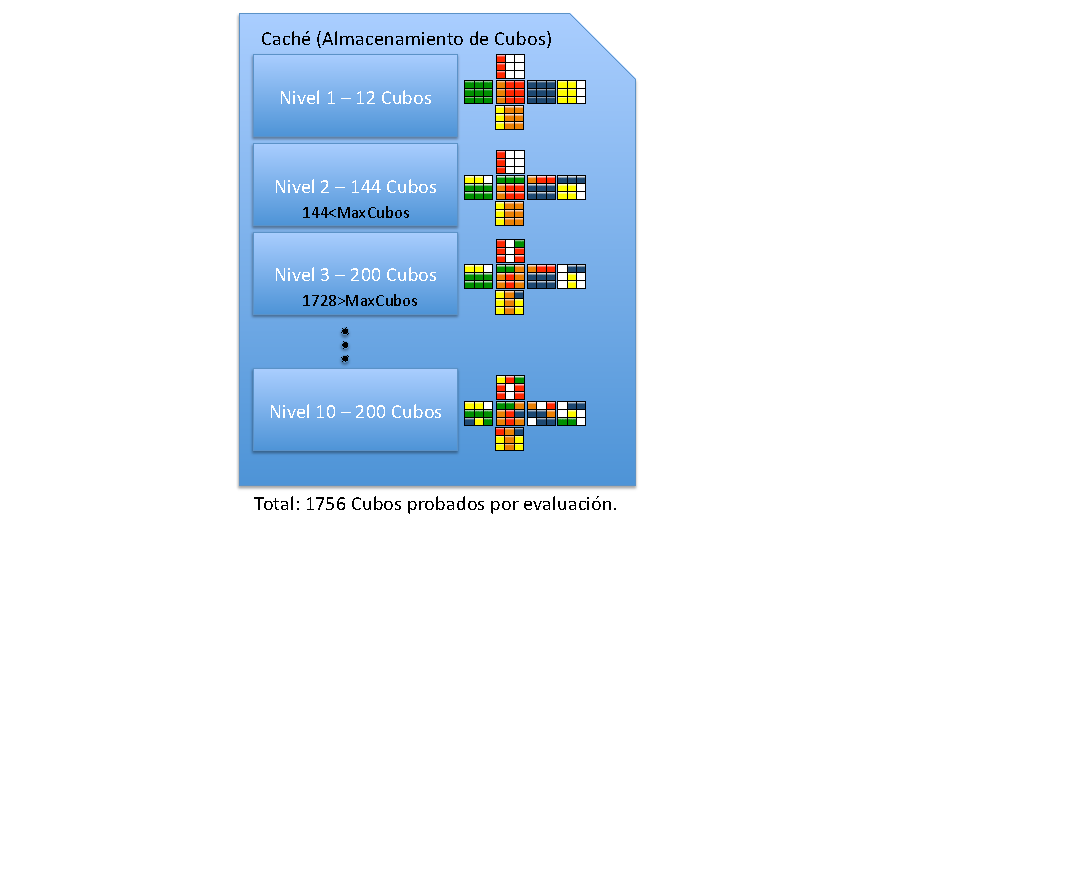
\includegraphics[width=0.45\textwidth]{figs/pdf/cache}
\caption{Almacen de cubos.}
\label{fig:cache}
\end{figure}


Además necesitamos saber la forma en la que probaremos los programas del conjunto
de entrenamiento. Como la estructura de los programas serán en forma de árbol, es
posible que en una sola iteración de la ejecución del árbol del programa no
dejemos expresar toda su capacidad resolutiva. Las sentencias que se encuentran
al principio del árbol del programa pueden no llegarse a ejecutar nunca ya que el
estado del cubo va cambiando a lo largo de la ejecución del árbol. Es por esto
que introducimos el concepto de iteraciones sobre el árbol del programa.

Para introducir las iteraciones en la ejecución del programa necesitaremos
especificar un número de iteraciones máximas para que el programa no itere
infinitamente. Además no nos interesa seguir iterando cuando hemos resuelto el
cubo. Con estas dos condiciones principales, el árbol del programa se ejecutará
una y otra vez hasta que alcancemos una solución o lleguemos a un límite de
iteraciones.

El límite de iteraciones se elegirá en función de los movimientos necesarios que
se requieren para resolver un cubo. Según estudios recientes, se cree que es
posible resolver cualquier cubo de Rubik en menos de 22 pasos. Suponiendo que al
menos se ejecuta un paso por iteración consideramos que 40 iteraciones es un
valor muy aceptable. Sin embargo, un número muy alto de iteraciones tiene un alto
coste computacional, por ello debemos elegir cautelosamente el valor adecuado de
iteraciones máximas. 

La figura \ref{fig:evaluacion} representa esquemáticamente el proceso de
evaluación.

\begin{figure}[t]
\centering
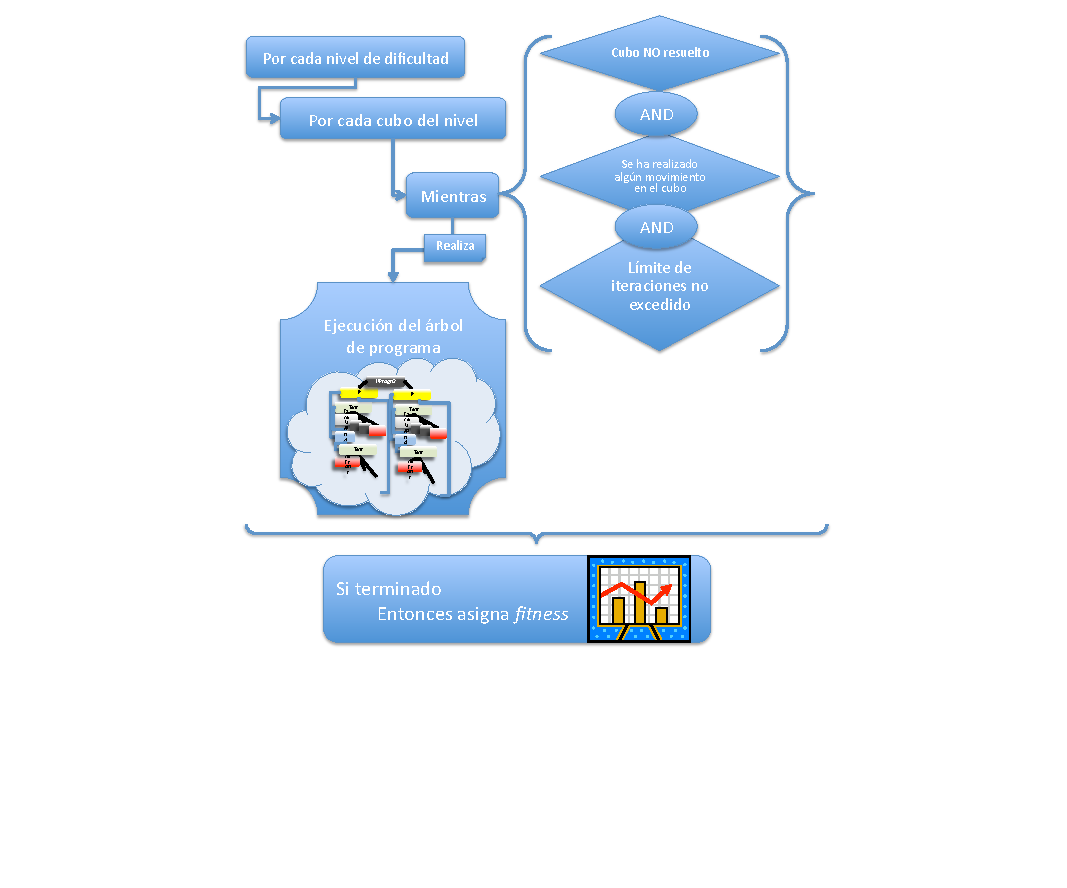
\includegraphics[width=0.85\textwidth]{figs/pdf/evaluacion}
\caption{Proceso de evaluación.}
\label{fig:evaluacion}
\end{figure}




\section{Optimización}\label{sec:optimizacion}

La programación evolutiva va estrechamente ligada a un gran consumo de recursos
computacionales. Sin embargo, no suele utilizar mucha memoria, por lo que
explotaremos al máximo el uso de la CPU generando caches y almacenando datos
calculados para que no tengan que volver a serlo.


\subsection{Reevaluación}\label{subsec:reevaluacion}

El primer paso gigantesco para acelerar el proceso de evaluación reside en no
reevaluar. Como los resultados perduran y siempre son los mismos en toda la
ejecución, no es necesario reevaluar. Así los individuos llevan un flag que
indica si han sido evaluados. Si no han sido evaluados, cuando se evalúen, se
ejecutará todo el proceso de evaluación. Si ya han sido evaluados, el proceso de
evaluación será omitido y se utilizarán los datos almacenados de la evaluación.

\subsection{Almacén de cubos}\label{subsec:almacen-cubos}

Para impedir emplear tiempo en generar cubos de Rubik cada vez que se evalua un
individuo. La muestra de cubos de Rubik de entrenamiento se generan al principio
del proceso de evolución. Así cuando evaluemos un programa, se extraerá un cubo
de Rubik del almacén de cubos. Además este sistema nos permite verificar la
calidad de los cubos que resuelven nuestros programas.

\subsection{Iteraciones inteligentes}\label{subsec:iteraciones-inteligentes}

Al introducir las iteraciones en la ejecución de los programas nos dimos cuenta
de que no siempre es necesario llegar al límite de iteraciones. Es posible que
aunque se ejecute el árbol, no se realice ningún cambio sobre el estado del cubo,
y, aunque en la siguiente iteración se vuelva a ejecutar el programa, el estado
del cubo va a ser el mismo. Por eso vamos a introducir un flag en el cubo que nos
indica si se ha cambiado el estado del cubo. Este flag se resetea en cada
iteración. Si en una iteración el flag indica que no se ha producido ningún
movimiento se escapará del bucle. No obstante, existen situaciones repetitivas,
periódicas, que son más difíciles de detectar, como por ejemplo, cuando en una
iteración se hace una acción y en la siguiente se deshace y esto se repite
infinitamente. Estos movimientos en bucle no llegan a ninguna parte. En nuestro
sistema ignoraremos estas situaciones ya que detectarlas consumiría una gran
cantidad de recursos que, si ajustamos correctamente el número de iteraciones
máximas, podemos paliar el efecto de esta situación no deseada.

\subsection{Motor del cubo de Rubik}\label{subsec:motor-cubo-rubik}

Para detectar las partes que ocupaban más tiempo del programa evolutivo, se
introdujeron temporizadores. Descubrimos que la capa de abstracción de posiciones
del cubo ocupaba gran parte del tiempo. Observamos, también, que existían
determinadas funciones equivalentes de rotación del cubo de Rubik que eran muchos
mas eficientes que otras, por lo que se reemplazaron las funciones existentes por
dichas funciones más óptimas para sacar el máximo rendimiento de ejecución.

Por otra parte, el cálculo de la entropía resultaba extrañamente pesado. La
explicación reside en que para calcular la entropía se genera un array que
contiene la situación de las pegatinas del cubo. Este array se calculaba cada vez
que se llamaba a la función de obtener las pegatinas. Ideamos un mecanismo que
mientras el cubo no cambie, el estado de las pegatinas se almacene en memoria, de
tal forma que sólo se computara el estado de las pegatinas cuando el cubo cambie
de estado.

\chapter{Implementación}\label{ch:implementacion}

\section{ECJ: Evolutionary Computation for Java}\label{sec:ecj}

Para la implementación del sistema evolutivo se utilizará la plataforma Java ECJ
desarrollada por el Dr. Sean Luke de la universidad de George Mason, diseñada
para la experimentación científica de esta rama \cite{MasonECJ}.

Se caracteriza por ser extremadamente modular y parametrizable. Esta plataforma
consta de diferentes librerías para cubrir casi todos los aspectos de la
computación evolutiva. Nosotros nos centraremos más en las librerías que se
centran en la programación genética.

Se eligió esta plataforma por que una de las normas del concurso es utilizar
Origin, plataforma de desarrollo multiproceso de sistemas evolutivos basada en
ECJ. Al ser una plataforma multiproceso hace que la información que podemos
extraer en las ejecuciones sea mínima. Además, la forma en que se utiliza es
idéntica a Origin con la excepción de unos pocos parámetros de configuración.

La clase principal que tiene ECJ es ec.Evolve. Esta clase se encarga de leer un
fichero de configuración del sistema y empezar la evolución. El fichero de
parámetros sirve para configurar los distintos aspectos de la evolución. Se
encarga tanto de las clases que se utilizarán, como de la estructura de los
árboles del lenguaje de los programas y de muchos otros parámetros de
configuración de las clases que intervienen en el proceso de evolución.

ECJ utiliza una estructura jerárquica de ficheros de configuración, de tal forma
que si queremos utilizar la librería de Koza para la programación genética,
simplemente tendremos que heredar del fichero de configuración de Koza y definir
ciertas propiedades especificas de nuestro problema. Esto se hace mediante la
siguiente línea:

parent.0 = ../../gp/koza/koza.params 

Sin embargo, para tener un control mucho más avanzado y personalizar ciertos
aspectos de nuestro sistema evolutivo necesitamos conocer algunos parámetros que
configuran aspectos cruciales de nuestra aplicación. El resto de parámetros los
encontraremos descritos en el anexo \ref{sec:ecj-params} de este proyecto ya
que es difícil encontrar documentación de estos parámetros.

La jerarquía de ficheros de configuración comienza con el fichero ec.params. Este
fichero configura los parámetros más simples de una ejecución evolutiva como por
ejemplo número de threads del proceso, semillas de números aleatorios, frecuencia
del checkpoint (fotografía de los programas en un punto de la evolución). El
siguiente fichero de la jerarquía es el fichero simple.params. Este fichero
asienta las bases de un proceso evolutivo, concretando las clases que
representarán a nuestros individuos, procesos de evaluación, reproducción,
estadísticas, etc.

El fichero koza.params, es el último fichero antes que el fichero de
configuración concreto de un sistema evolutivo como por ejemplo el nuestro. Este
fichero concreta los aspectos que son necesarios para poder evolucionar
programas. El Dr. Sean se ciñe estrictamente al sistema evolutivo descrito por
Koza \cite{Koza:1992}, no obstante, siempre es posible cambiar el
comportamiento de ciertos módulos para adaptarlos a nuestro sistema.

El sistema de Koza consta de las siguientes características. El fitness será un
número el cual el individuo perfecto adquiere el valor 0 y el peor individuo
tendrá el valor infinito.

Los individuos constarán de un solo árbol de programa. Además este árbol puede
tener restricciones gramaticales.

La forma de reproducción que se va utilizar será una combinación de cruzamiento y
clonación con probabilidades de 0.9 y 0.1 respectivamente. Esto significa que el
operador de reproducción que predominará será el cruzamiento.

Para elegir a los progenitores se utilizará la selección por torneo. Se realizará
un torneo de un número determinado de individuos escogidos aleatoriamente de la
población. El ganador será elegido como padre. La madre será elegida de igual
forma. Para la clonación servirá el mismo método, pero sin cruzamiento.

Para seleccionar el nodo que se intercambiará con el progenitor en el cruzamiento
se limitará la profundidad a un determinado número de nodos, además de elegirse
aleatoriamente dentro del límite establecido. Podremos también condicionar la
búsqueda del nodo eligiendo la probabilidad de seleccionar un nodo terminal, un
nodo no-terminal o incluso la raíz del árbol.

En el proceso de mutación se utilizará “Point Mutation” donde se seleccionará un
nodo aleatorio dentro de una profundidad límite establecida, con un número de
intentos establecido. Una vez que se selecciona el nodo de la misma forma que en
el cruzamiento, se generará un subárbol completamente aleatorio utilizando el
operador grow.

Además en la inicialización de los árboles combinaremos el método grow y el
método full que previamente hemos descrito en el estado del arte.

Una vez descrito el funcionamiento del sistema, explicaremos concretamente los
parámetros principales que utilizaremos a lo largo del proyecto y que nos han
servido para realizar múltiples pruebas:

\begin{itemize}
\item $gp.koza.xover.tries$ : Es el número de intentos que el sistema realiza
para que la operación de cruzamiento se realice con éxito, es decir, sintánticamente correcto. Si no se consigue una combinación adecuada en la operación de cruzamiento se clonarán a los individuos. Por defecto, el número de intentos es 1.
\item $gp.koza.xover.maxdepth$ : Es la profundidad máxima permitida para buscar
subárboles compatibles en ambos individuos para realizar el intercambio en el proceso de cruzamiento. 
\item $select.tournament.size$ : Es el número de individuos que tienen los
torneos del sistema. Cuanto más alto, más probabilidades de escoger al mejor individuo. Sin embargo, cuantas más veces se escoja siempre el mismo individuo, la diversidad empobrecerá.
\item $gp.koza.mutate.tries$ : Número de intentos de mutar a un individuo.
\item $gp.koza.mutate.maxdepth$ : Profundidad máxima para mutar un punto del
árbol de programa. 
\item $gp.koza.grow.min-depth$ y $gp.koza.grow.max-depth$ : La
profundidad máxima que el operador grow utilizará a la hora de generar un árbol estará comprendida entre estos dos valores.
\end{itemize}

\subsection{Origin}\label{subsec:origin}


Origin es el sistema que convierte a ECJ en un sistema multiproceso para ser
utilizado en Frontier. Frontier es un grid de ordenadores alrededor del mundo
desarrollado por Parabon. Para pertenecer a este grid, el único paso a seguir es
instalar la herramienta de Frontier en tu ordenador, y tu ordenador empezará a
formar parte de este grid.

Parabon, la empresa que se encuentra detrás de estas dos tecnologías, combinó la
potencia de investigación de ECJ con la potencia computacional de Frontier, dando
lugar al sistema Origin. Aunque Origin nació de ECJ, actualmente son productos
distintos, mantenidos por empresas diferentes, y cada vez son productos que
divergen más.

Aunque un requerimiento del concurso es utilizar Origin para evolucionar nuestros
programas, tuvimos múltiples problemas desde el inicio: Origin se encuentra en
fases muy tempranas de su desarrollo. Esto hace que ciertos aspectos del sistema
no se encuentran muy desarrollados. Por ejemplo, la ejecución del sistema se
realizaba mediante un script, dificultando utilizar cualquier herramienta de
depuración, al contrario que ECJ, el cual se ejecuta directamente llamando a una
clase Java. Por otro lado, parte del código de Origin esta oculto y no podemos
acceder a él, por lo que es difícil predecir en ciertas ocasiones el resultado de
ciertas acciones. En tercer lugar, en sus últimas versiones dejaron de soportar
el modelo generacional (master-slave), en el cual el ordenador que lanza  la
ejecución se encarga de coordinar el funcionamiento, para soportar exclusivamente
el modelo de estado fijo (oportunistic), donde el comportamiento esta mucho más
distribuido, dificultando enormemente la recogida de estadísticas e información
de funcionamiento del sistema, el cuál es fundamental para el desarrollo de
aplicaciones. Por último, al ser un sistema distribuido, los procesos tienen que
esperar a ser ejecutados según las prioridades de Frontier, por lo que, para
ciertos casos pequeños de prueba el overhead de utilizar un sistema distribuido
es demasiado grande.

Debido a todos estos problemas que presenta Origin decidimos trasladar nuestro
trabajo a ECJ. Gratamente comprobamos que no tuvimos que cambiar prácticamente
nada del código existente. Además ECJ permitía el uso de breakpoints, código
abierto, múltiples hilos de ejecución, ejecución local (podemos inspeccionar
cualquier rincón de nuestro programa) y no dependía de ningún artefacto
prioritario que retrasara la ejecución de nuestros procesos.

Origin es una herramienta orientada a la ejecución: mejora el rendimiento de
nuestra aplicación. No obstante, se encuentra en desarrollo y por lo tanto esta
sujeto a grandes cambios (y fallos), y, por último, resulta muy difícil utilizar
con la herramienta cuando se trata de un trabajo de investigación ya que
necesitamos obtener la máxima información posible de nuestras ejecuciones y
Origin falla en este aspecto.

\subsection{Extensiones a ECJ}\label{subsec:mod-ecj}

Al implementar nuestro sistema tuvimos una serie de problemas que nos obligaron a
realizar ciertas modificaciones a la plataforma ECJ. El problema surgió al
intentar utilizar un lenguaje con fuertes restricciones gramaticales. Estas
restricciones no permiten colocar cualquier nodo como hijo de otro nodo en el
momento de generar árboles. El resultado: desbordando la pila de memoria de la
máquina virtual de Java. Para explicar el motivo del fallo recordemos el método
de generación de árboles full. Este método construía árboles de programa mediante
nodos no-terminales hasta llegar a la profundidad máxima, en donde sólo utilizaba
nodos terminales (vease sección \ref{subsubsec:inittree}). El problema es que en
nuestro lenguaje no siempre es posible colocar un nodo terminal como hijo de otro
nodo. Esto provoca que cuando el método full se encuentra en la fase de colocar
nodos terminales y no encuentra ninguno que pueda utilizar, elige aleatoriamente
entre los nodos no-terminales que gramaticalmente encajan. El desbordamiento de
la pila de memoria se produce al escoger nodos no-terminales que producen que el
árbol se expanda infinitamente. Esto es debido a que el método full desconoce de
antemano qué nodos no-terminales son los que acaban terminando la rama de un
árbol. Es por ello que hay que informar al método full de cuales son los nodos
no-terminales que pueden llevar a terminar la rama de un árbol.

Este es el caso de las funciones de nuestro sistema como move y test. Estas
funciones son símbolos no-terminales que generan sólo un nivel más de profundidad
en la rama del árbol. En este nivel adicional del árbol se encuentran los
argumentos de llamada a la función. Por lo tanto, este tipo de nodos debería
considerarse como un nodo terminal, ya que si se usa este nodo no-terminal, se
producirá la parada de la expansión del árbol.


El sistema no es consciente de estos hechos y por lo tanto no sabe qué nodo
escoger en el caso de que se quiera parar la expansión del árbol solo puede
escoger entre símbolos no-terminales en función de su aridad. En nuestro caso, en
ciertas ocasiones existe el 50\% de posibilidades de que se escoja un símbolo que
puede duplicar el número de nodos o  un símbolo que pare la expansión. Si escoge
el nodo que duplica el número de nodos de la rama, tendrá dos nuevas
oportunidades de volver a escoger el nodo que sigue expandiendo el árbol. Esto
hace muy probable que el sistema cree un árbol infinito, desbordando la memoria
disponible.

La solución consistió en extender la funcionalidad del sistema de tal manera que
desde el fichero de parámetros podamos especificarle qué nodo posee cualidades de
terminal aunque sea no-terminal. Para hacer esto, sobrescribimos la clase GPNode
para leer este flag del fichero de parámetros. Además cambiamos la funcionalidad
de las clases ec.gp.koza.KozaBuilder, ec.gp.koza.HalfBuilder y
ec.gp.koza.GrowBuilder para que tuvieran en cuenta este flag a la hora de
clasificar nodos terminales y no-terminales. De esta forma pudimos generar
árboles sin que se produjera ningún error.

La segunda gran modificación que realizamos en el sistema sirvió para poder
utilizar nuestro propio sistema de fitness. De esta forma, sobrescribiendo la
función que compara dos individuos, podemos decirle al sistema nuestra
preferencia a la hora de elegir.

La ultima modificación es una modificación obligada, es decir, la propia
documentación del framework ECJ recomienda realizar estos cambios. Esta
modificación cambia la manera que tiene el sistema de sacar datos de
funcionamiento e imprimir estadísticas. De esta forma podemos obtener una
información mucho más rica del sistema para poder encontrar la solución a nuestro
problema.

\section{Cubetwister y el cubo de Rubik}\label{sec:cubetwister}


El modelo computacional del cubo de Rubik va a ser el especificado en el concurso. 
Para representar el cubo de Rubik en el ordenador utilizaremos la librería de
Randelshofer (cubetwister.jar) \cite{Randelshofer}, en la versión 1.0.3.2.
Existe una importante diferencia entre la versión 1 y la versión 2, también disponible en la Web,
sobre todo en la nomenclatura de las caras. La numeración de las caras será la
siguiente: la cara frontal será la 0, la derecha, la 1; la inferior, la 2; la
trasera, la 3; la izquierda, la 4; y por último la superior, la 5
(figura \ref{fig:carasrubik}).
 
\begin{figure}[t]
\centering
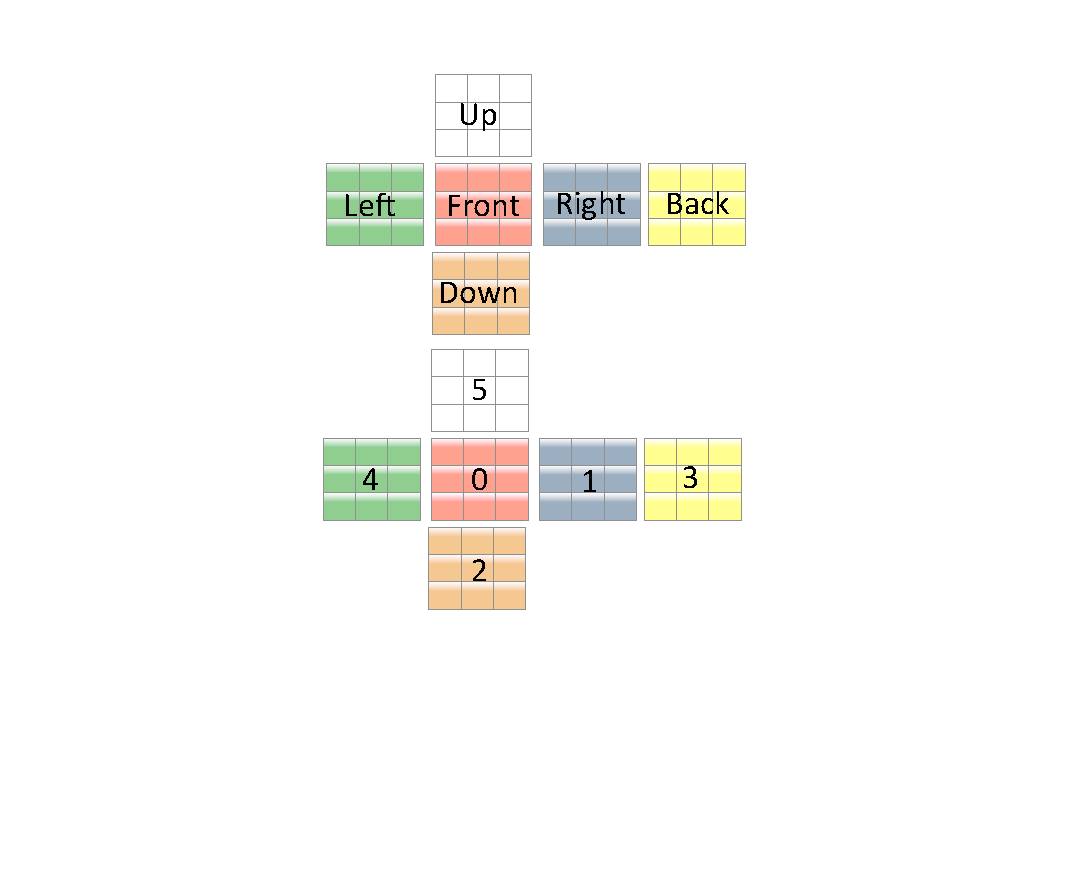
\includegraphics[width=0.55\textwidth]{figs/pdf/carasrubik}
\caption{Asignación numérica de las caras
del cubo de rubik..}
\label{fig:carasrubik}
\end{figure}

Además, internamente, para situarnos dentro de una cara, utilizaremos la
representación gráfica matemática (figura \ref{fig:rubikfaceposition}), donde
X0 e Y0 se situarán en la parte superior izquierda de la cara. No obstante el eje de ordenadas estará invertido, siendo la casilla X0 Y0 la casilla que esta en la esquina superior izquierda y la casilla X2Y2 la casilla de la esquina inferior derecha.

\begin{figure}[t]
\centering
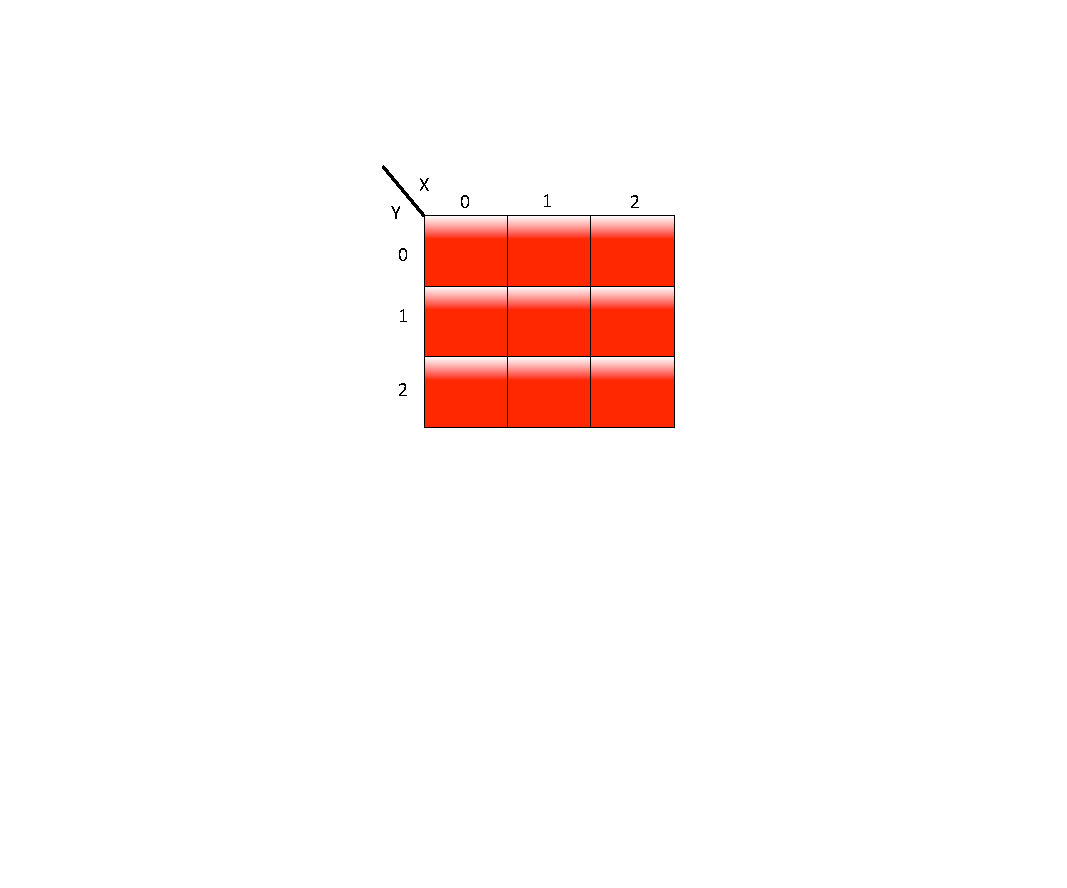
\includegraphics[width=0.45\textwidth]{figs/pdf/rubikfaceposition}
\caption{Asignación numérica de las posiciones de las casillas de una cara
del cubo de rubik.}
\label{fig:rubikfaceposition}
\end{figure}


\clearpage

\section{Diagrama de clases}\label{sec:dia-clases}

Las figuras \ref{fig:package-rubik}, \ref{fig:package-direction},
\ref{fig:package-color} y \ref{fig:package-func} representan los diagramas de
clase de la aplicación.

\begin{figure}[bct]
\centering
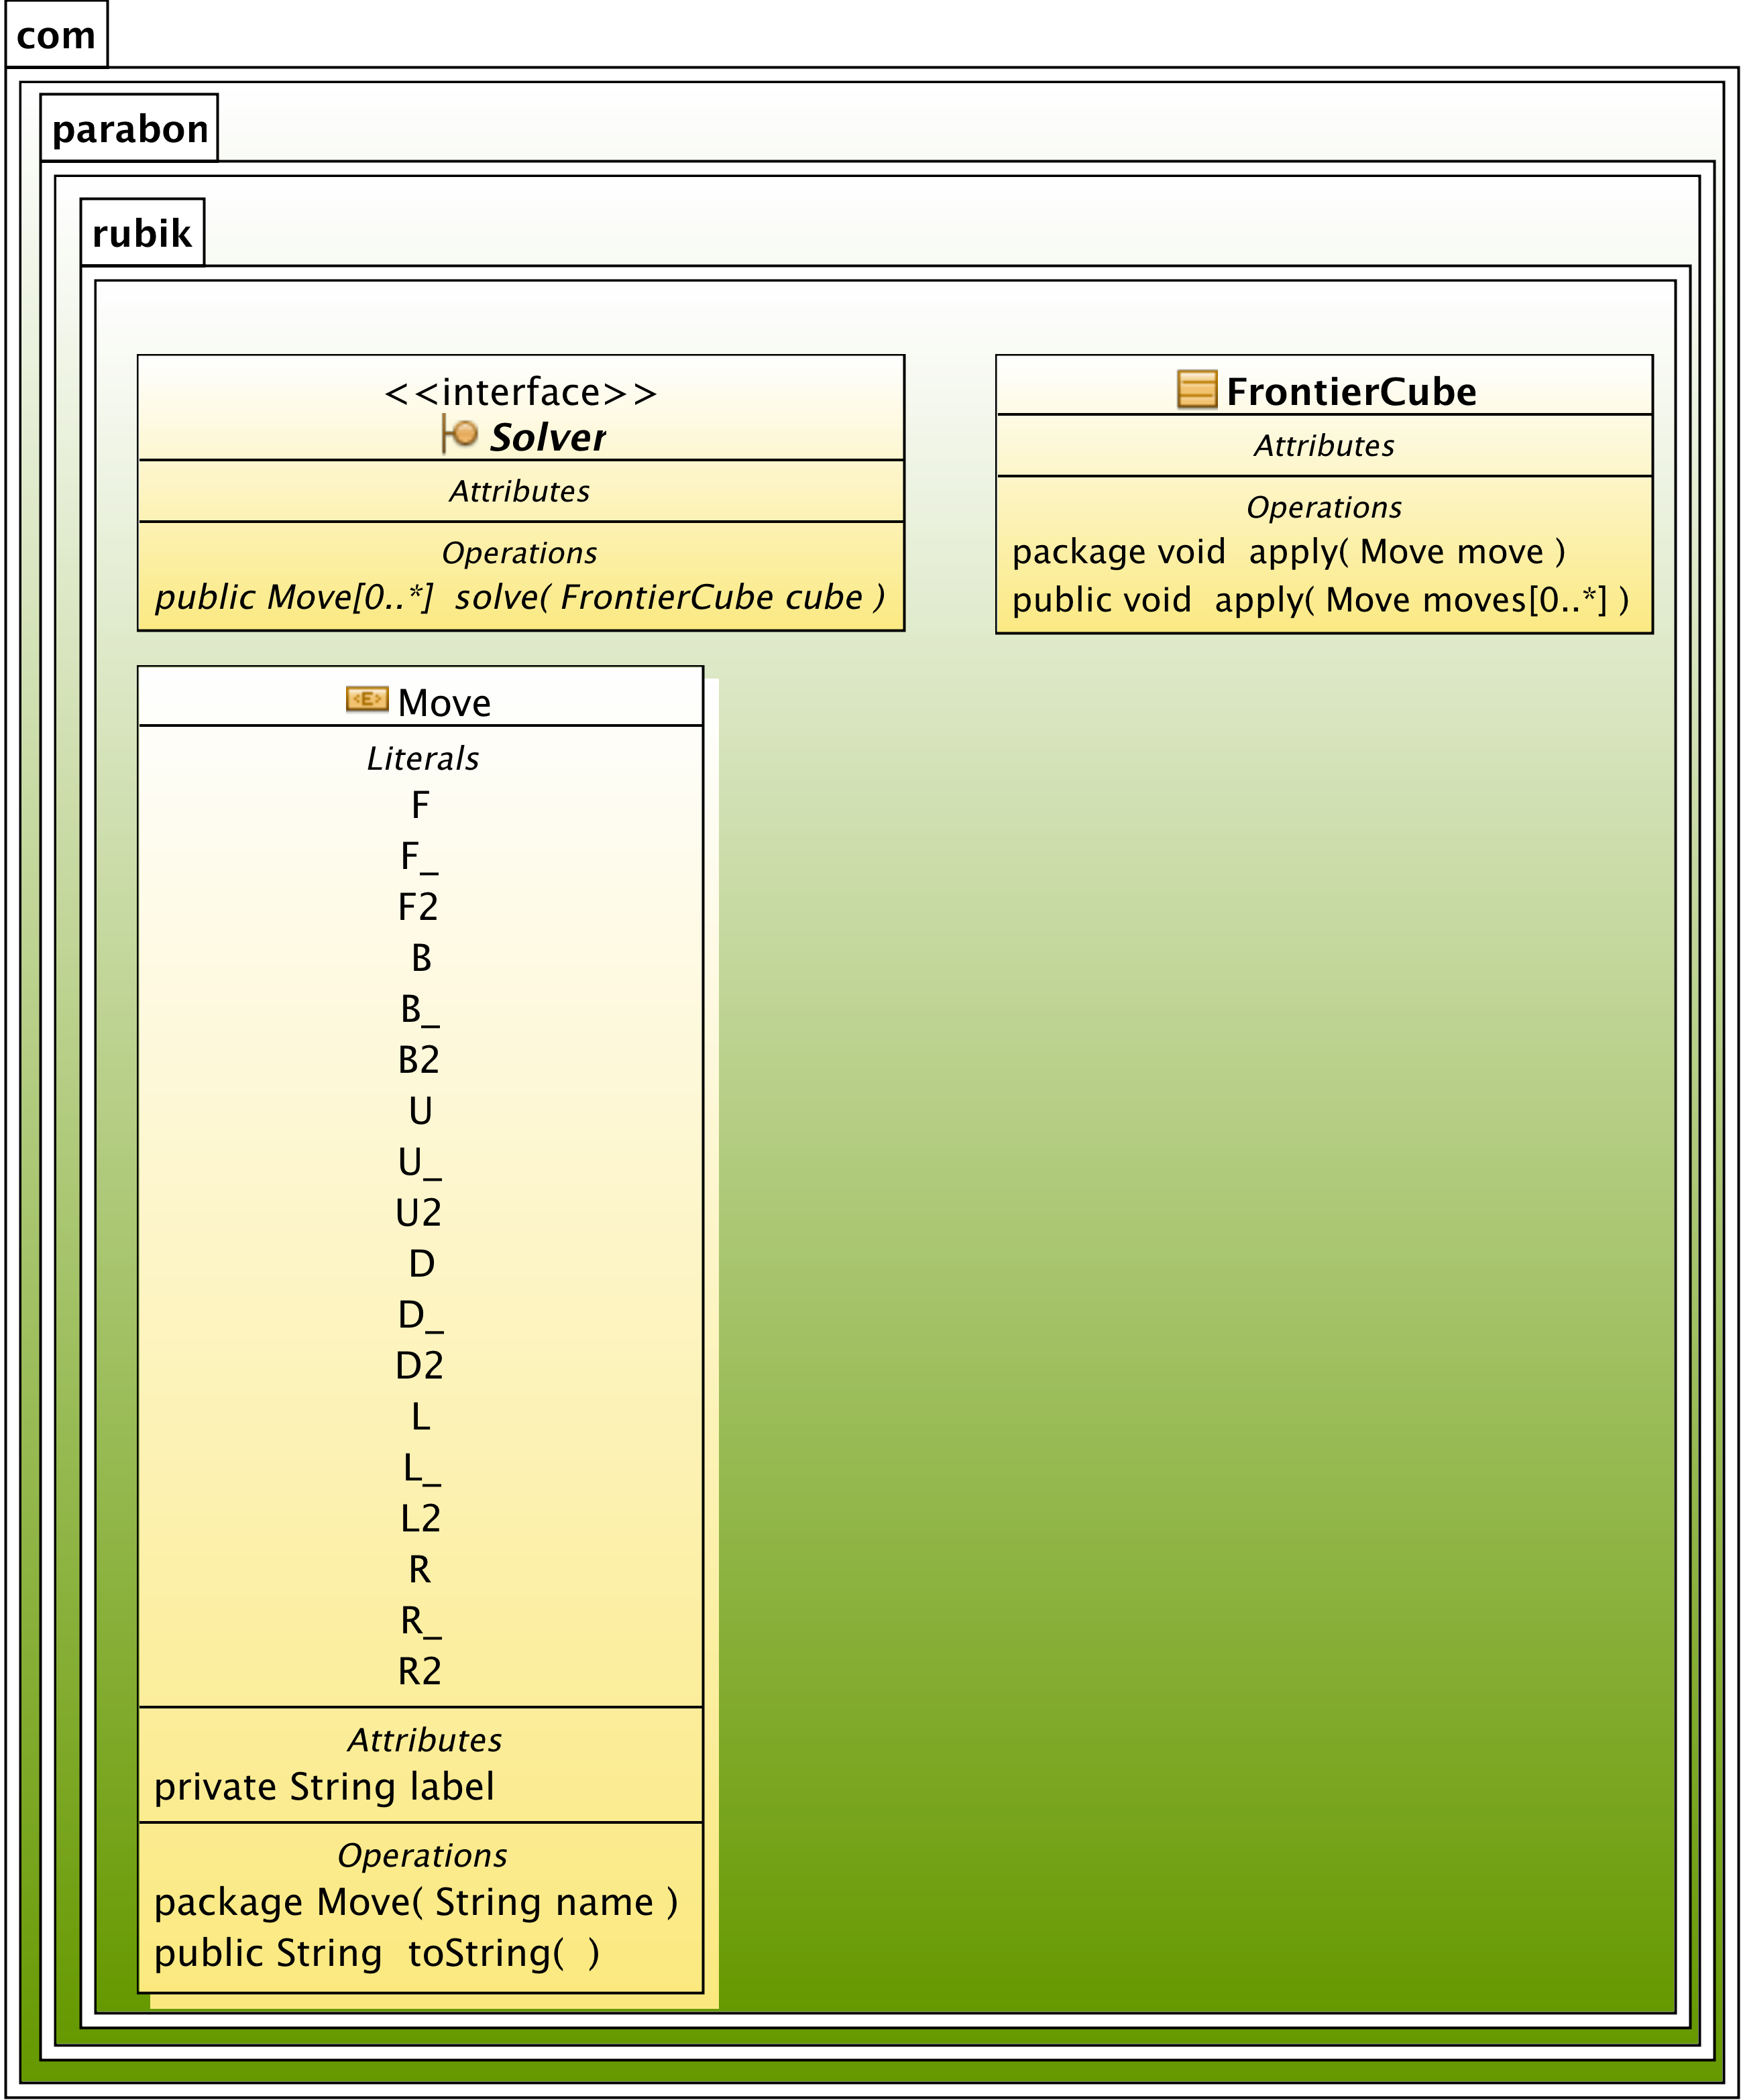
\includegraphics[scale=0.10]{figs/classes/rubik}
\caption{Paquete com.parabon.rubik}
\label{fig:package-rubik}
\end{figure}

\begin{figure}[cbt]
\centering
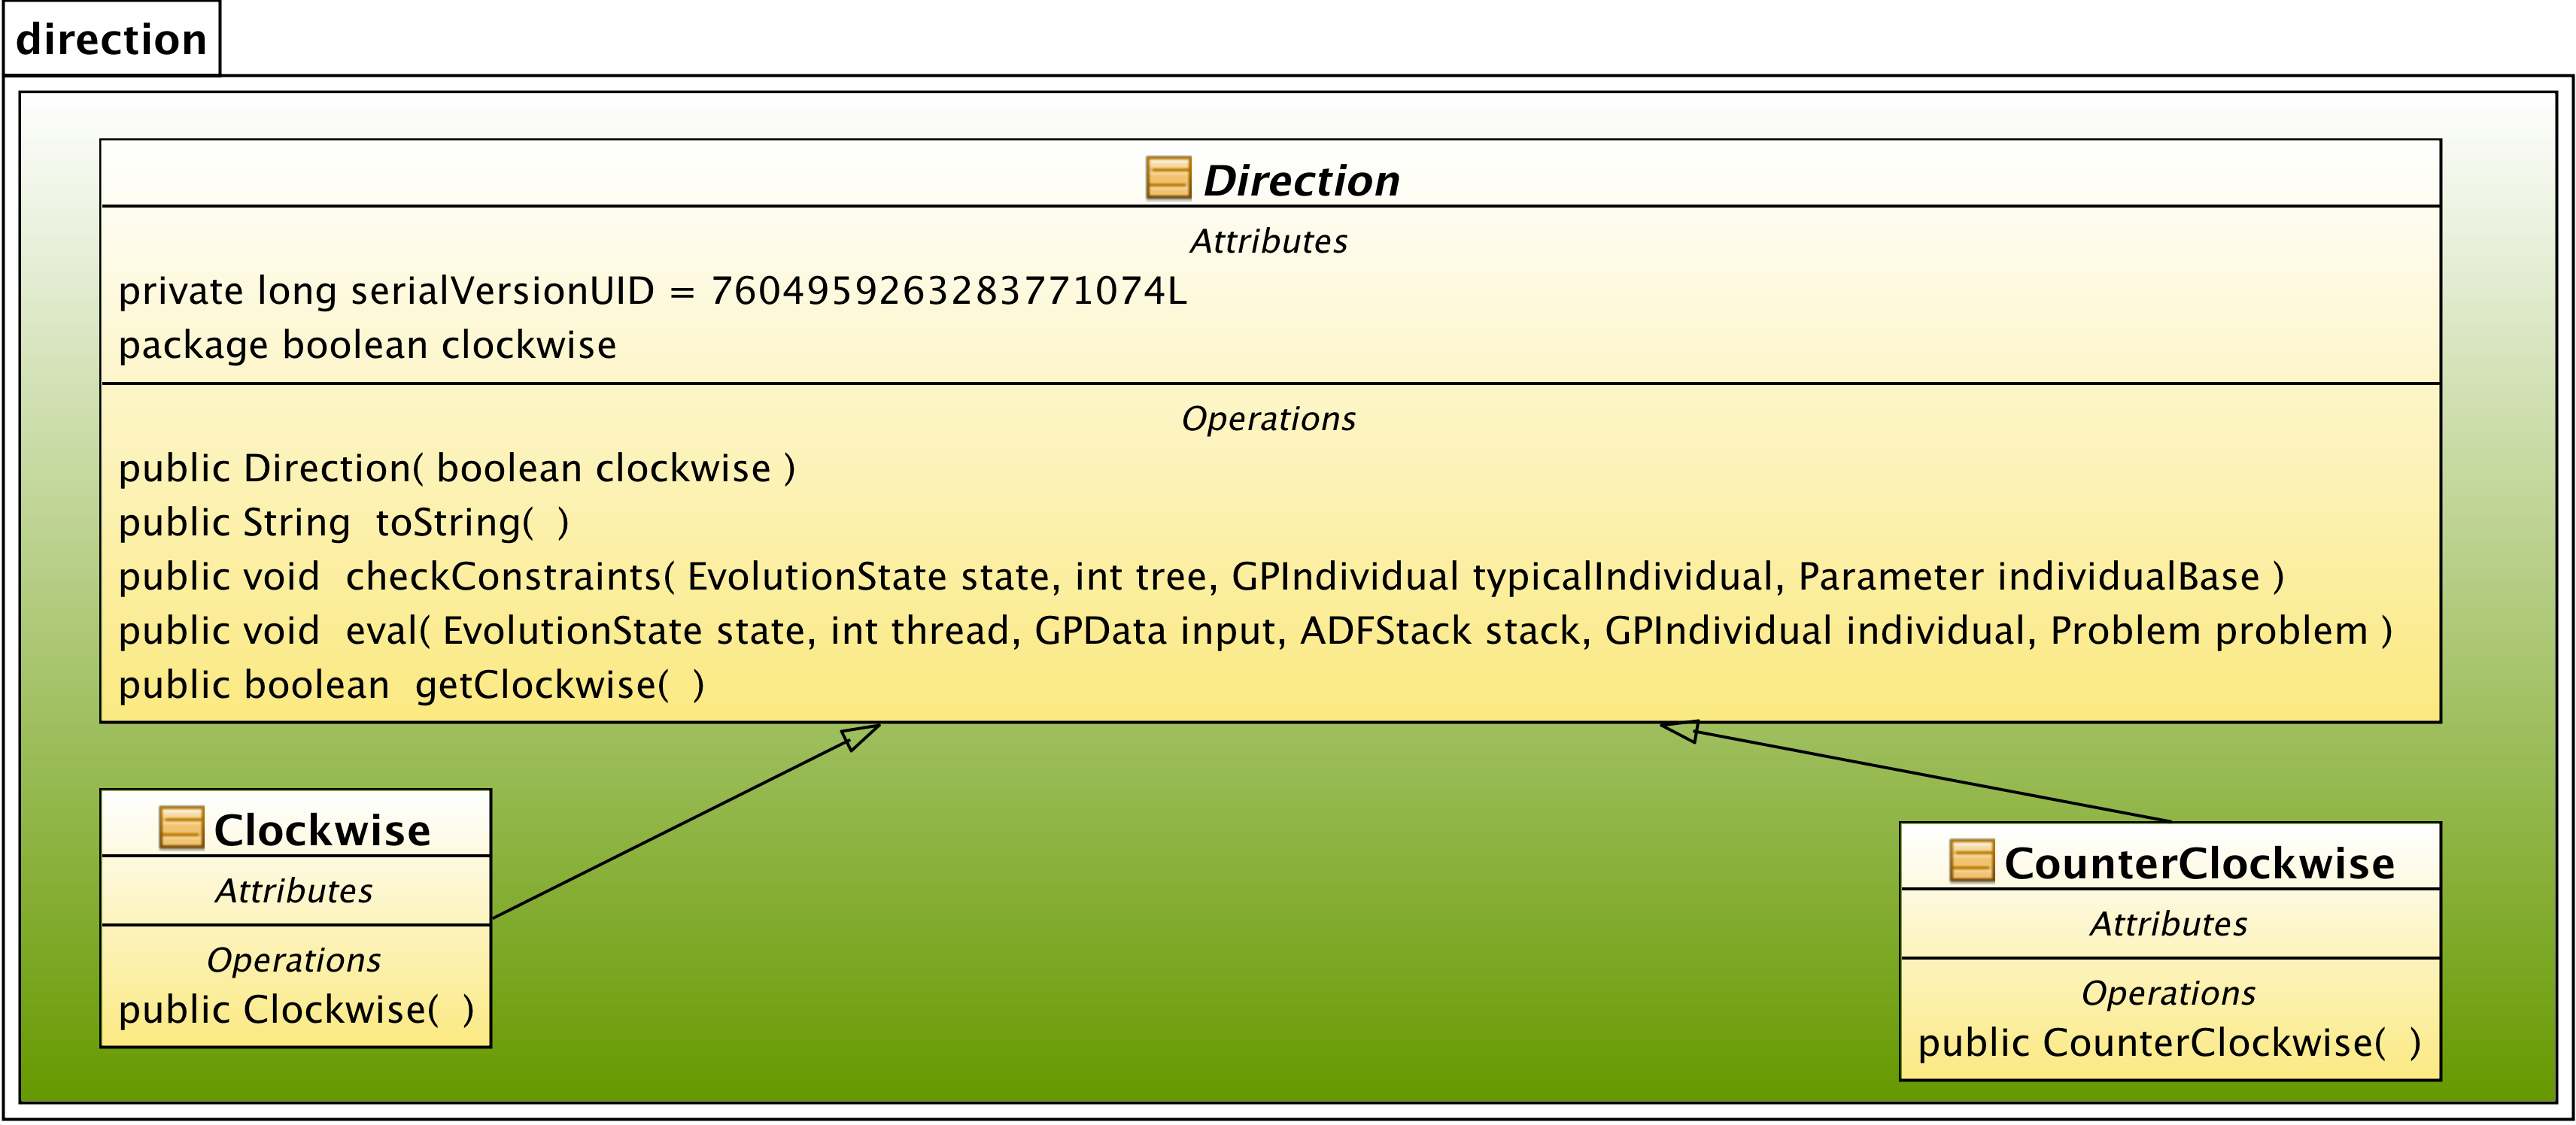
\includegraphics[scale=0.12]{figs/classes/direction}
\caption{Paquete direction.}
\label{fig:package-direction}
\end{figure}

\begin{figure}[ctb]
\centering
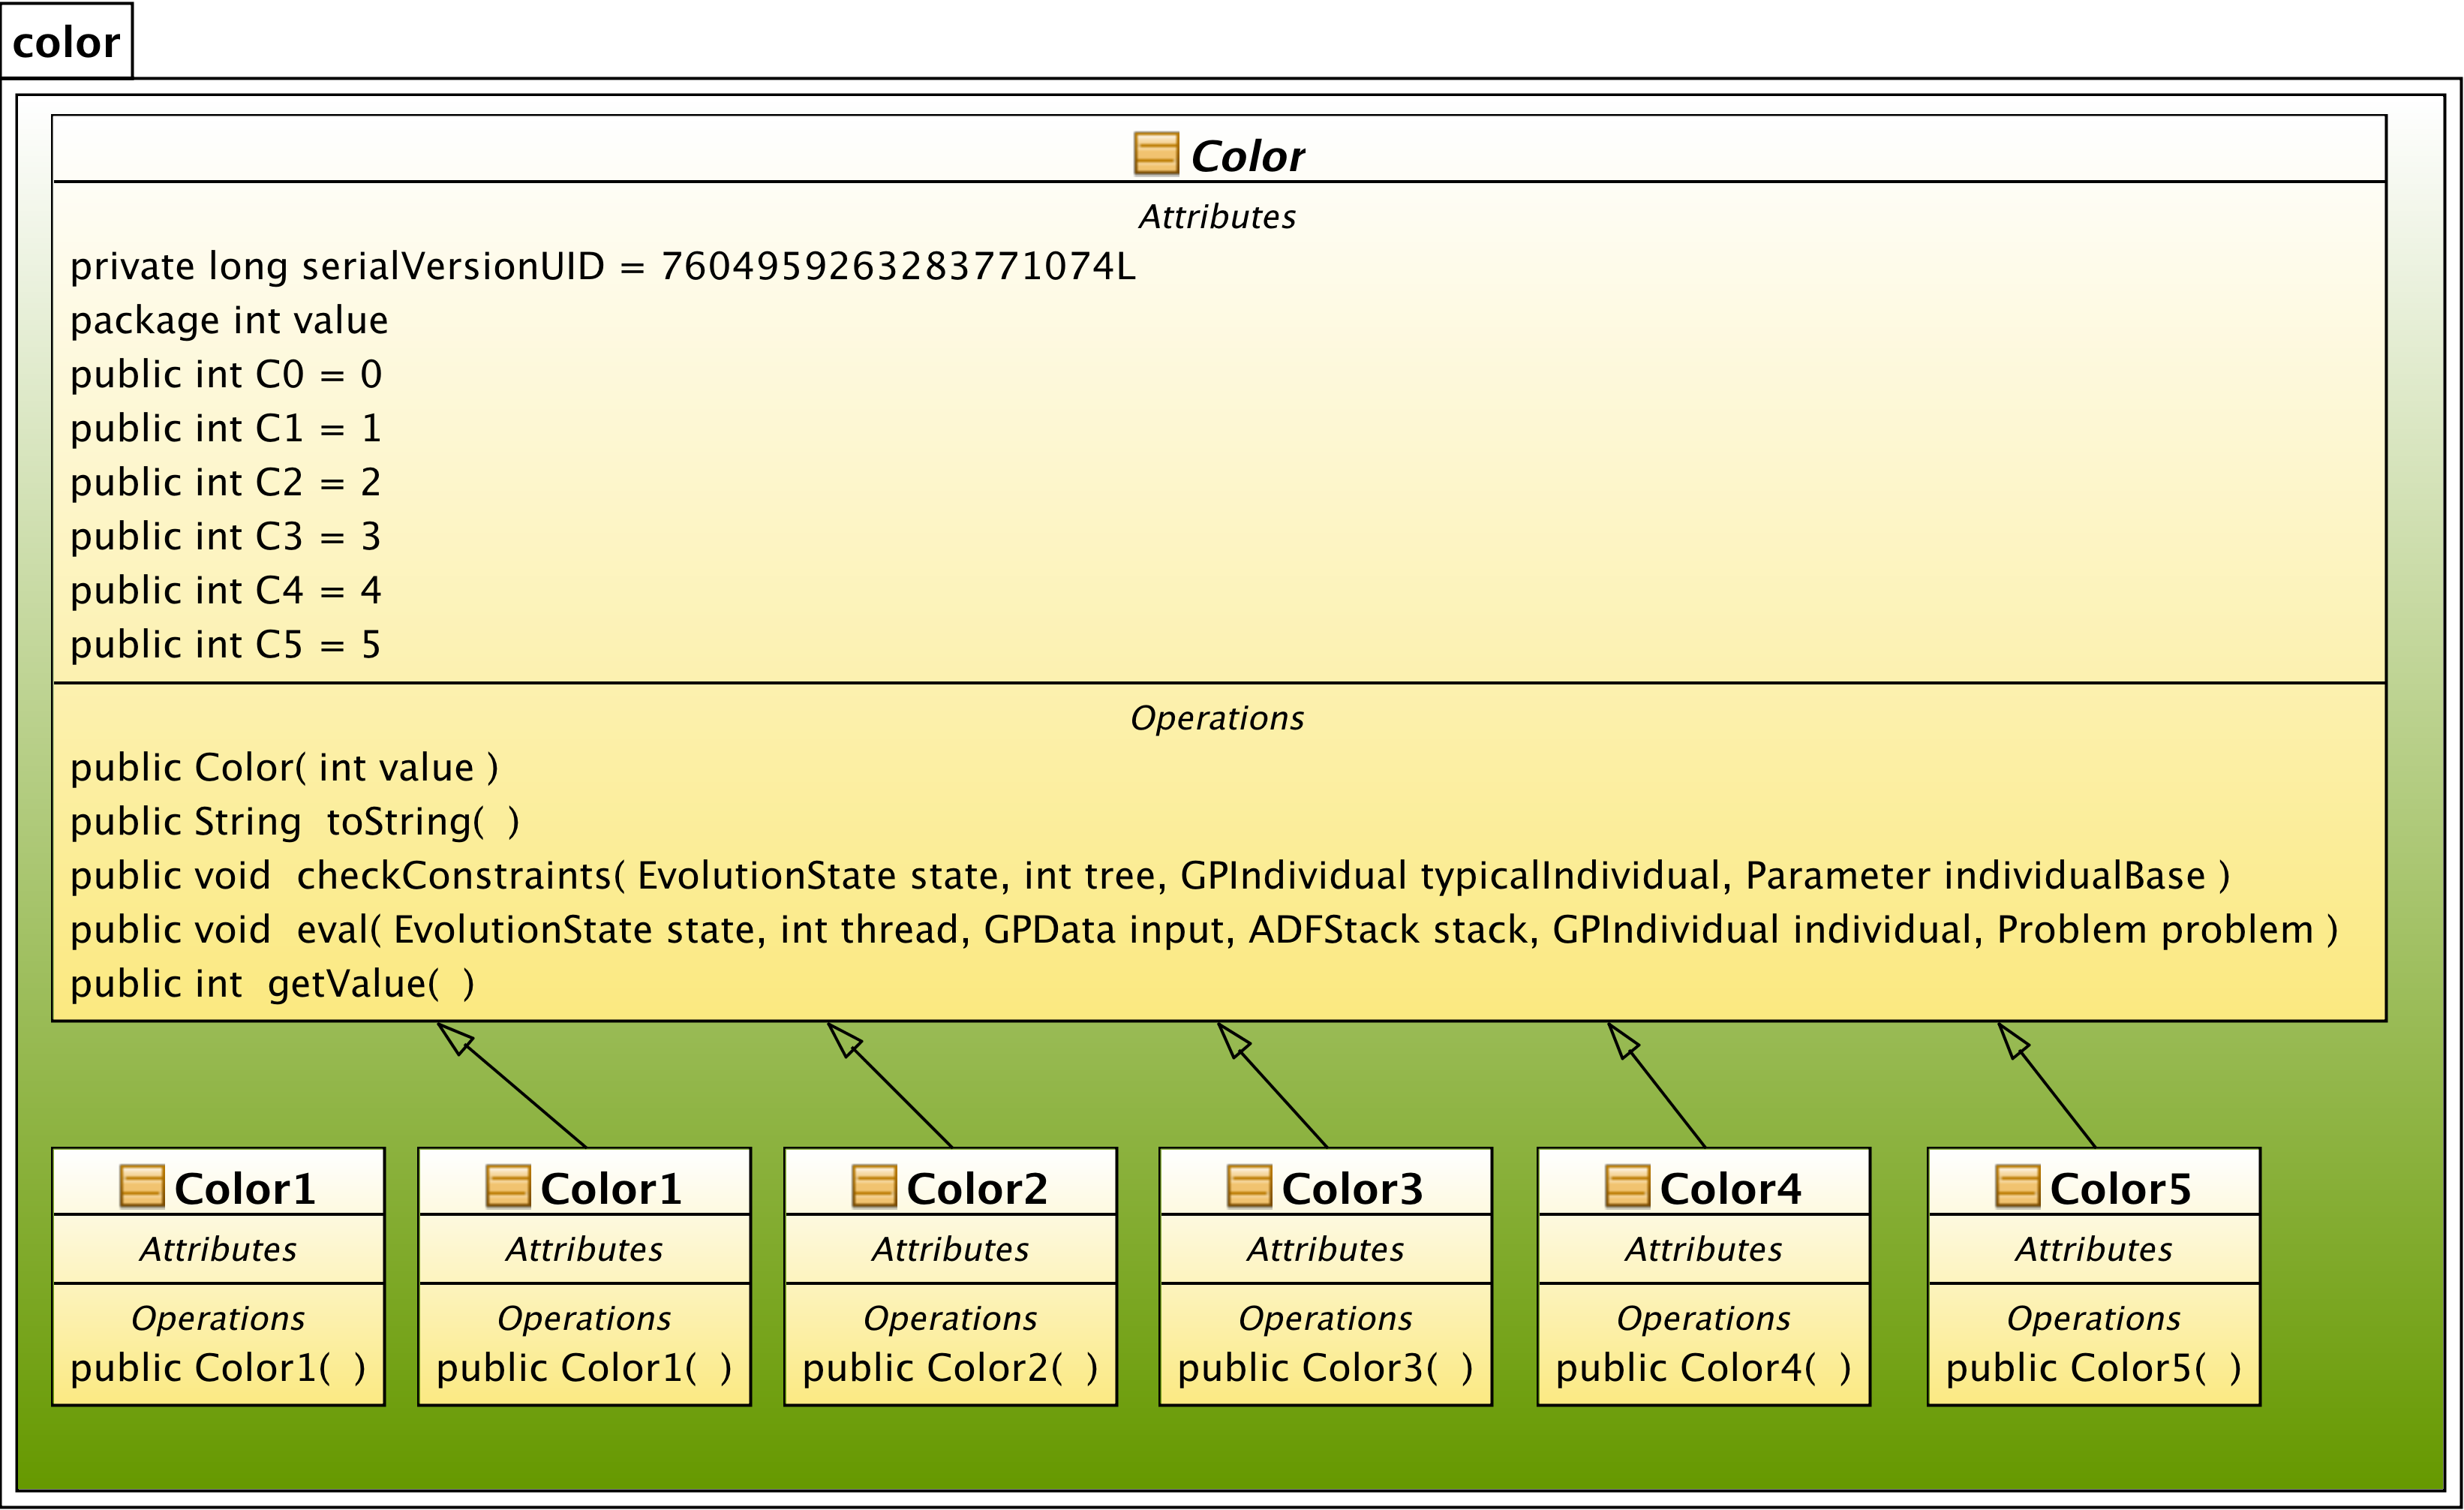
\includegraphics[scale=0.12]{figs/classes/color}
\caption{Paquete color.}
\label{fig:package-color}
\end{figure}

\begin{figure}[cbt]
\centering
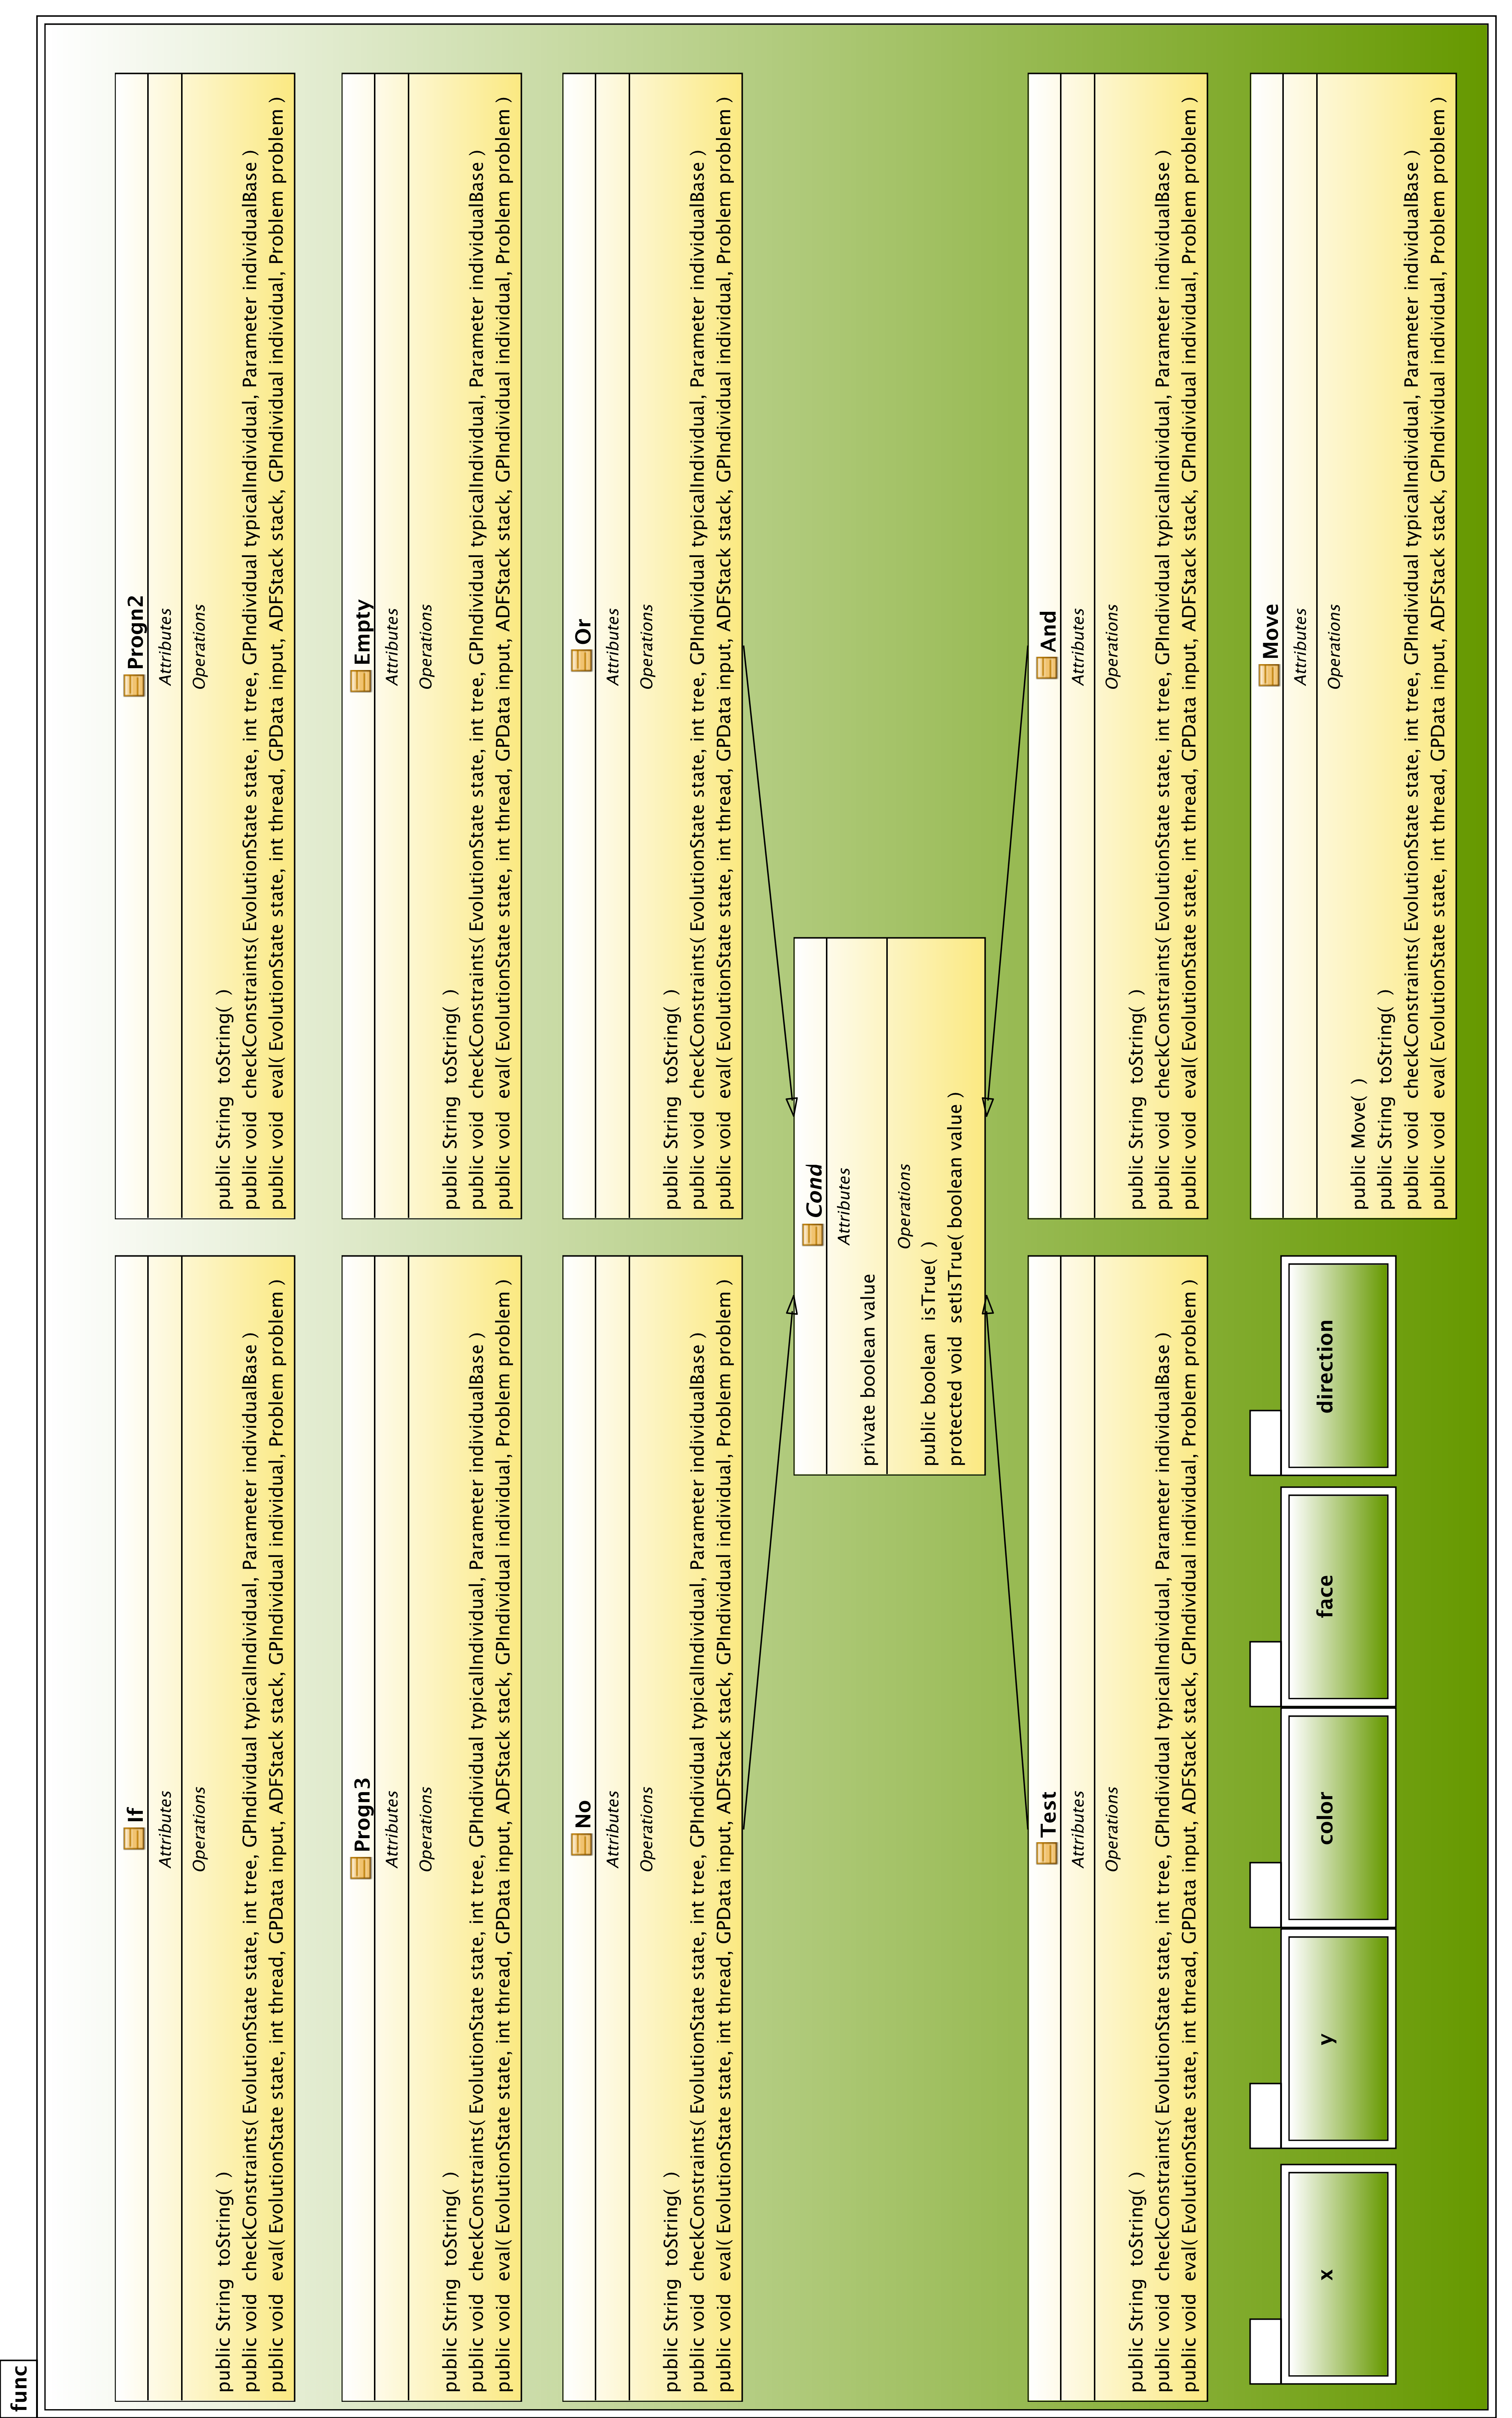
\includegraphics[scale=0.09]{figs/classes/func}
\caption{Paquete func.}
\label{fig:package-func}
\end{figure}


\chapter{Pruebas y Resultados}\label{ch:pruebasyresultados}

La naturaleza del algoritmo propuesto hace difícil determinar la configuración
inicial del mismo ya que la forma de encontrar la máxima efectividad del mismo es
mediante la experimentación con distintos valores de sus parámetros.

Por este motivo se hace necesario realizar un conjunto de experimento que
permitan entender la influencia de los parámetros en el desempeño del algoritmo.
En particular analizaremos la influencia de:

\begin{itemize}
  \item Número de intentos al realizar el cruzamiento.
  \item Número de individuos del torneo.
  \item Número de intentos de mutación.
  \item Profundidad máxima del método grow.
  \item Profundidad máxima en el cruzamiento.
  \item Profundidad máxima en la mutación.
  \item Factor Fitness
\end{itemize}
 

En cada caso ejecutaremos el algoritmo dejando fijo el resto de parámetros y
modificando el parámetro bajo estudio. Al tratarse de procesos aleatorios cada
ejecución con la misma configuración puede ser completamente diferente, sin
embargo, al hacer la media de varias ejecuciones, podremos sacar conclusiones
objetivas sobre el rendimiento del algoritmo con la configuración. Por esto, se
procede a lanzar 10 ejecuciones de cada configuración. Después  de las
ejecuciones analizaremos la media de los resultados para compararla con la media
de otras ejecuciones.

\section{Número de intentos al realizar
cruzamiento}\label{sec:p-intentos-cruzamiento}

Como se describe en la sección \ref{para:crossover}, a la hora de realizar el
cruzamiento se pueden permitir una serie de intentos para obtener un árbol
válido. En caso de que no se obtenga un árbol válido en el número de intentos
especificados, no se llevará a cabo el cruzamiento. Con este experimento queremos
determinar cual es el valor más conveniente para el problema que nos hemos
planteado.

\begin{table}[tb]
\caption{Valores de los parámetros para el número de intentos al realizar el
cruzamiento.}
\label{tab:cross-tries}
\centering
\begin{tabular}{lcccc}
\toprule
  &\textbf{Prueba 1} & \textbf{Prueba 2} & \textbf{Prueba 3} &\textbf{Prueba
  4}\\
\midrule
gp.koza.xover.tries    & $1$ & $10$ & $100$ & $1000$ \\
\bottomrule
\end{tabular}
\end{table}


En la tabla \ref{tab:cross-tries} se encontrarán los valores de los parámetros
que se han utilizado para este caso. La figura \ref{subfig:p-crosstries-best}
muestra la evolución de los valores de fitness del mejor individuo a través de
las distintas iteraciones para los distintos valores del parámetro analizado. De
manera similar la figura \ref{subfig:p-crosstries-mean} presenta los valores que
toma el fitness medio de la población a medida que avanza la ejecución del
algoritmo. Como complemento a las figuras anteriores, en la figura
\ref{subfig:p-crosstries-nodes} se puede apreciar el número medio de nodos de los
árboles de programa de la población. Finalmente la figura
\ref{subfig:p-crosstries-time}  se refiere al consumo de recursos
computacionales durante la ejecución del programa.


El análisis de las figuras anteriores nos permite concluir que la cantidad de
intentos (verde) resulta más conveniente porque produce el mejor desempeño, y
además se puede observar que el valor del parámetro no implica mayores costes
computacionales que otros de peor calidad.

Resulta interesante constatar que el número de nodos se mantiene en rangos
similares en la primera parte de la ejecución del algoritmo pero a partir de un
punto empiezan a divergir.

Como resultado de este experimento podemos concluir que el valor más conveniente
de la cantidad de intentos para realizar con éxito el cruzamiento es $1000$
intentos.


\begin{figure}[cbt]
  \centering
  \subfloat[Calidad de los mejores individuos]{
  	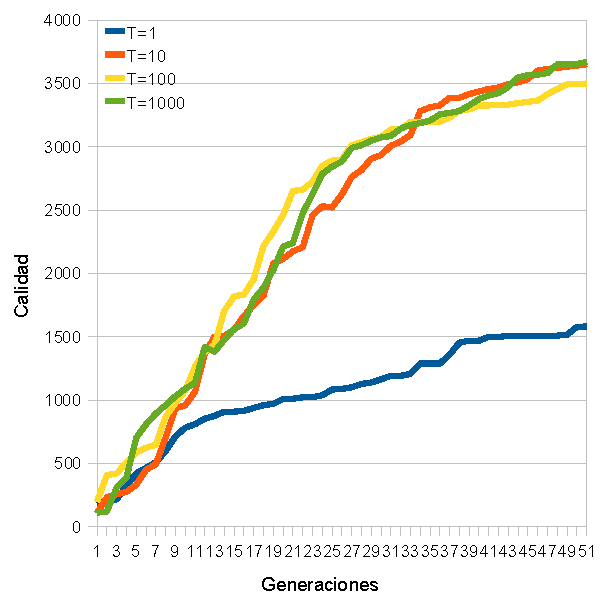
\includegraphics[width=0.4\textwidth]{figs/graphs/CrossTriesBest}
	\label{subfig:p-crosstries-best}
  }                
  \subfloat[Calidad media de la población]{
  	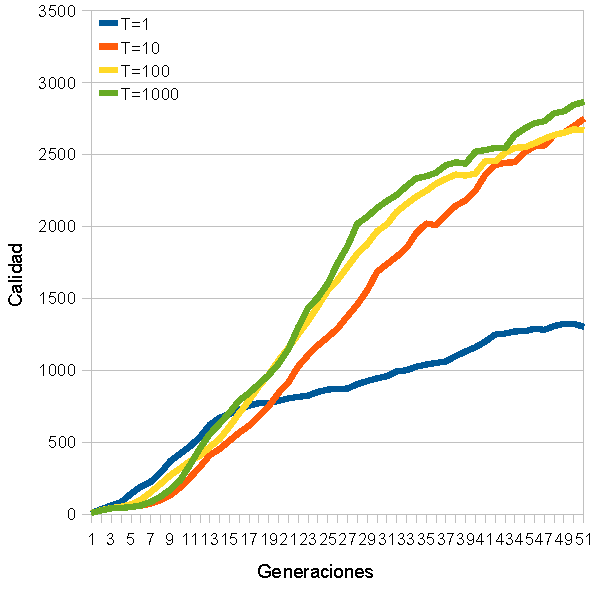
\includegraphics[width=0.4\textwidth]{figs/graphs/CrossTriesMean}
	\label{subfig:p-crosstries-mean}%
  }
  \quad
  \subfloat[Número de nodos medio de la población]{
  	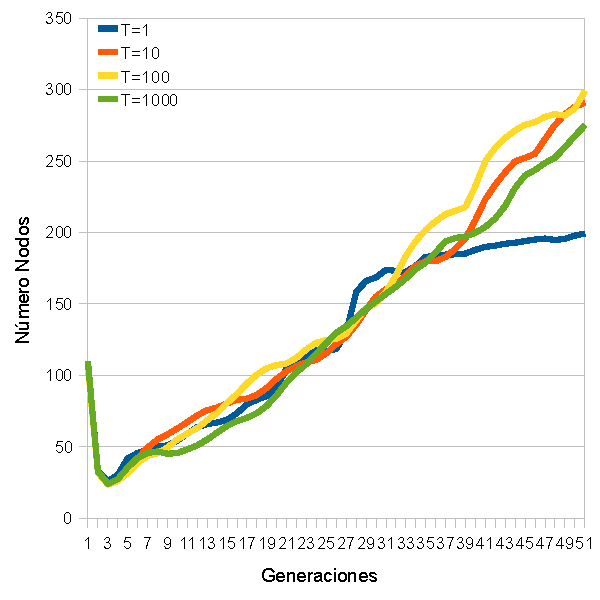
\includegraphics[width=0.4\textwidth]{figs/graphs/CrossTriesNodes}
	\label{subfig:p-crosstries-nodes}%
  }
  \subfloat[Tiempo de las ejecuciones]{
  	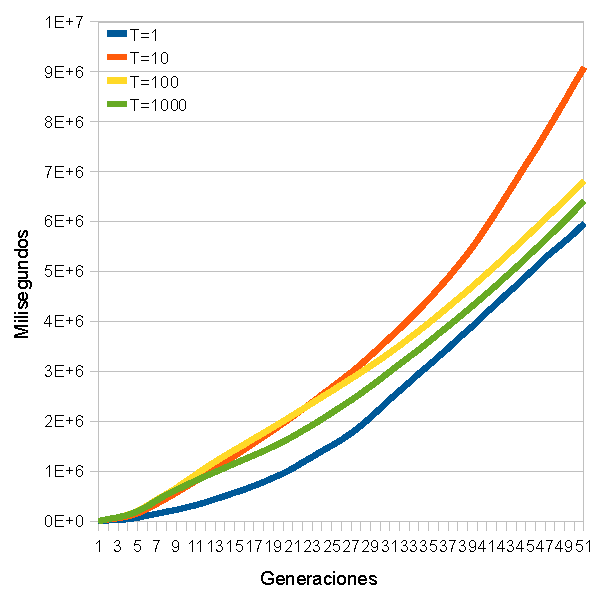
\includegraphics[width=0.4\textwidth]{figs/graphs/CrossTriesTime}
	\label{subfig:p-crosstries-time}%
  }
  \centering
\caption{Número de intentos de realizar
cruzamiento ($T$)}
\label{fig:p-crosstries}
\end{figure}

%  
\section{Número de individuos del torneo}\label{sec:p-individuos-torneo}

El número de individuos del torneo, descrito en la sección Y, es el número de
individuos que entran en el torneo de selección del padre y la madre para
producir un nuevo individuo.

El resultado esperado es que, al aumentar el número, la probabilidad de escoger
al individuo más apto es mayor. De esta forma, el individuo más apto ganará
siempre los torneos, distribuyendo su código genético en la siguiente generación.
Por ello, la diversidad de la población disminuirá.

Por el contrario, si el número de individuos en el torneo es muy bajo, las
probabilidades de que en el torneo aparezcan individuos más aptos es menor. Por
ello, es posible que se pierdan individuos muy aptos que deberían haber tenido
descendencia.

\begin{table}[cbt]
\caption{Valores de los parámetros para el número de individuos del torneo.}
\label{tab:individuos-torneo}
\centering
\begin{tabular}{lccc}
\toprule
  &\textbf{Prueba 5} & \textbf{Prueba 6} & \textbf{Prueba 7}\\
\midrule
select.tournament.size &  $2$  & $4$ & $7$ \\
\bottomrule
\end{tabular}
\end{table}


Siguiendo la estructura presentada en la sección \ref{sec:p-individuos-torneo}
(tabla de parámetros \ref{tab:individuos-torneo}) tanto la figura
\ref{subfig:p-tournsize-best} que muestra la calidad media como la figura \ref{subfig:p-tournsize-mean} que muestra la calidad máxima, nos
indican que el mejor desempeño lo ofrece el valor 4 para el número de individuos
del torneo. Este hecho confirma nuestra previsión de los resultados, ya que un
valor bajo como 2 ofrece muy poco rendimiento, y un valor alto como 7 no supera
la calidad obtenida por el valor 4.

El número de nodos (figura \ref{subfig:p-tournsize-nodes}) nos índica que
el valor 2 produce árboles con pocos nodos, el valor 4 produce árboles de tamaño
medio y el valor 7 produce los árboles con un mayor número de nodos. En este
caso, la exigencia computacional (figura \ref{subfig:p-tournsize-time}) va a la
par del número de nodos.


\begin{figure}[cbt]
  \centering
  \subfloat[Calidad de los mejores individuos]{
  	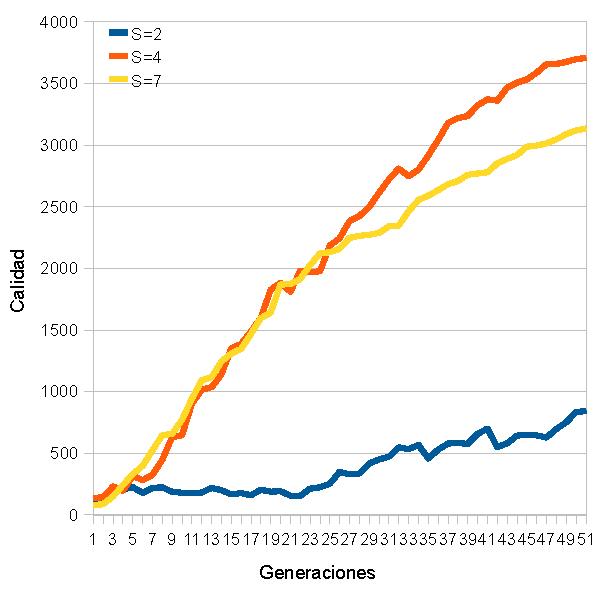
\includegraphics[width=0.4\textwidth]{figs/graphs/TournSizeBest}
	\label{subfig:p-tournsize-best}
  }                
  \subfloat[Calidad media de la población]{
  	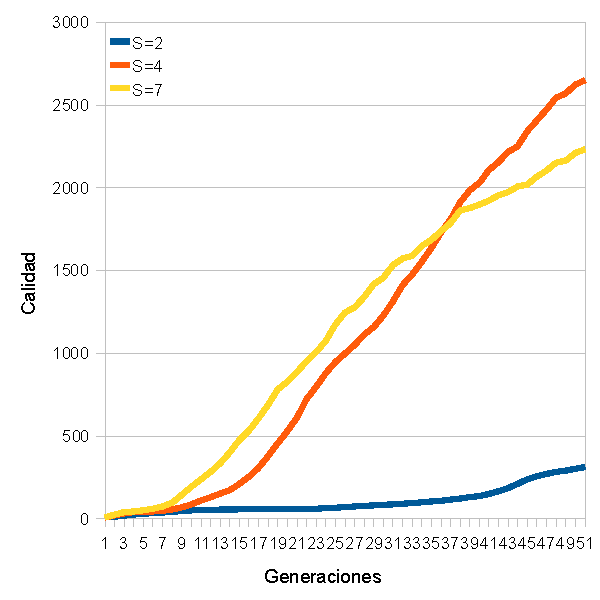
\includegraphics[width=0.4\textwidth]{figs/graphs/TournSizeMean}
	\label{subfig:p-tournsize-mean}%
  }
  \quad
  \subfloat[Número de nodos medio de la población]{
  	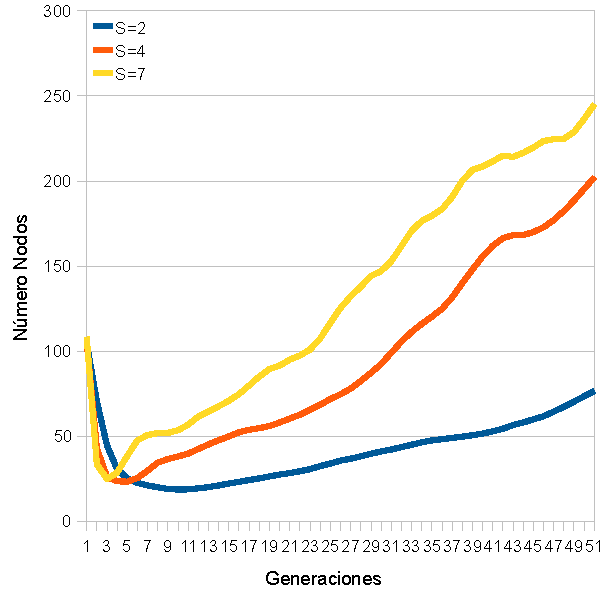
\includegraphics[width=0.4\textwidth]{figs/graphs/TournSizeNodes}
	\label{subfig:p-tournsize-nodes}%
  }
  \subfloat[Tiempo de las ejecuciones]{
  	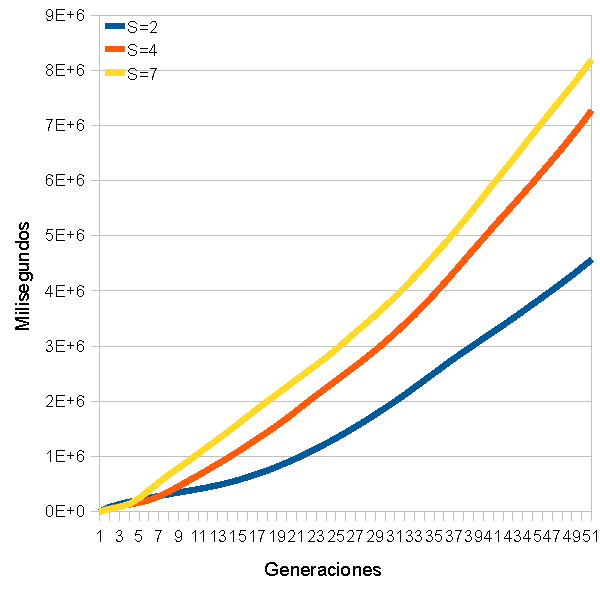
\includegraphics[width=0.4\textwidth]{figs/graphs/TournSizeTime}
	\label{subfig:p-tournsize-time}%
  }
  \centering
\caption{Número de individuos del torneo ($S$)}
\label{fig:p-crosstries}
\end{figure}


\section{Número de intentos de mutación}\label{sec:p-intentos-mutacion}

El número de intentos de mutación es el número de intentos del algoritmo para
generar una mutación válida en el árbol de programa, donde una mutación válida es
aquella que consigue generar un árbol sintácticamente correcto. En nuestro
algoritmo, la mutación seleccionará un punto en el árbol aleatoriamente y
generará un subárbol también aleatoriamente.

El número de intentos de mutación representa la probabilidad de mutación. Así, 0
significa que no existirá mutación; 1 que hay mutación pero con muy baja
probabilidad. Sin embargo, no podemos asegurar nunca un 100\% de probabilidad de
mutación, ya que siempre es posible superar un número de intentos (por alto que
sea) sin encontrar una mutación válida.

\begin{table}[tb]
\caption{Valores de los parámetros para el número de intentos de mutación.}
\label{tab:mutate-tries}
\centering
\begin{tabular}{lccc}
\toprule
  &\textbf{Prueba 8} & \textbf{Prueba 9} & \textbf{Prueba 10}\\
\midrule
gp.koza.mutate.tries & $0$ &  $1$  & $10$ \\
\bottomrule
\end{tabular}
\end{table}

Una vez realizadas las pruebas con los valores indicados en la tabla
\ref{tab:mutate-tries}, los resultados revelan que el mejor desempeño (figuras
\ref{subfig:p-mutatetries-best} y \ref{subfig:p-mutatetries-mean}) se encuentra
cuando el número de intentos de mutación es 10. Además es posible que un valor
más elevado pueda conseguir mejor desempeño, sin embargo, para ser un estudio
científico riguroso tendríamos que realizar otro estudio en detalle para
optimizar este parámetro.

La mejora del rendimiento (figura \ref{subfig:p-mutatetries-time}) debido al
aumento de la probabilidad de mutación puede deberse a que al principio del proceso evolutivo aparece una reducción general de
nodos (figura \ref{subfig:p-mutatetries-nodes} generaciones 1-4) y por ello la
diversidad se reduce. La mutación  es un operador que aporta nueva diversidad a
la población en cualquier punto de la evolución. Por ello creemos que la mutación
es necesaria para la evolución en este problema, y, no obstante, probablemente
exista un límite superior donde la mutación no beneficie a la calidad de los
individuos.

\begin{figure}[cbt]
  \centering
  \subfloat[Calidad de los mejores individuos]{
  	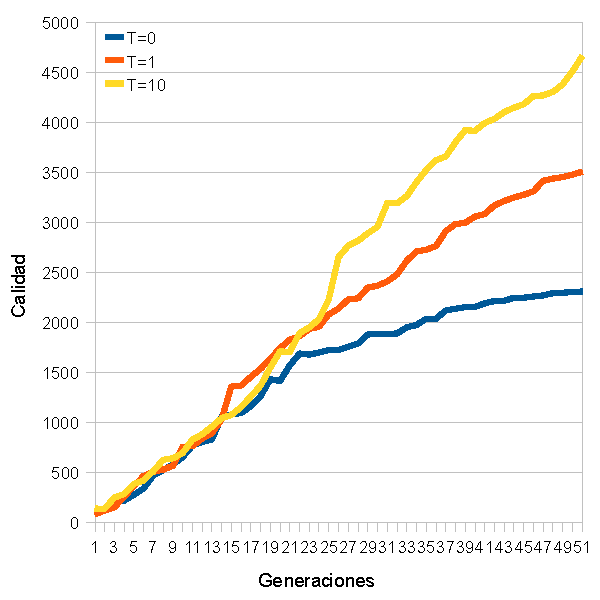
\includegraphics[width=0.4\textwidth]{figs/graphs/MutateTriesBest}
	\label{subfig:p-mutatetries-best}
  }                
  \subfloat[Calidad media de la población]{
  	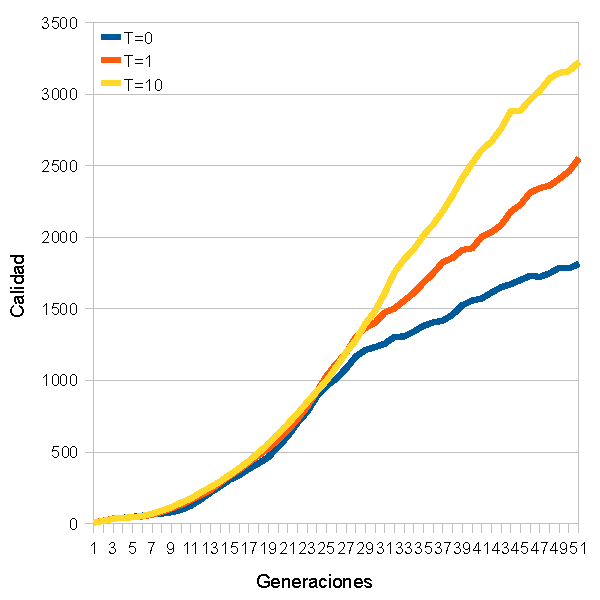
\includegraphics[width=0.4\textwidth]{figs/graphs/MutateTriesMean}
	\label{subfig:p-mutatetries-mean}%
  }
  \quad
  \subfloat[Número de nodos medio de la población]{
  	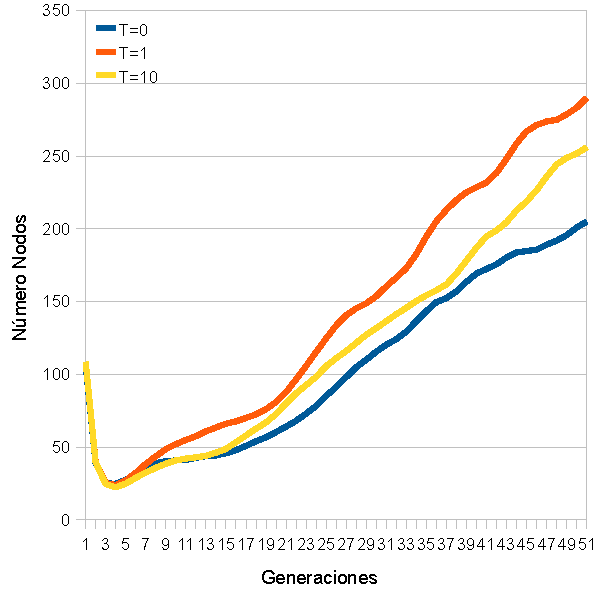
\includegraphics[width=0.4\textwidth]{figs/graphs/MutateTriesNodes}
	\label{subfig:p-mutatetries-nodes}%
  }
  \subfloat[Tiempo de las ejecuciones]{
  	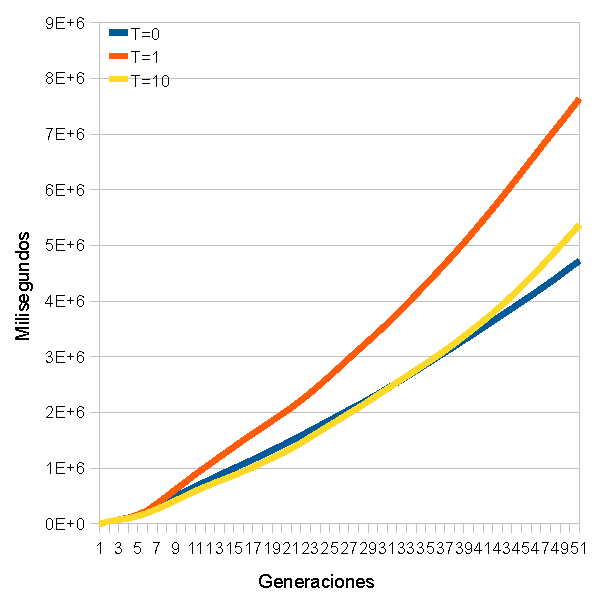
\includegraphics[width=0.4\textwidth]{figs/graphs/MutateTriesTime}
	\label{subfig:p-mutatetries-time}%
  }
  \centering
\caption{Número de intentos de mutación ($T$)}
\label{fig:p-crosstries}
\end{figure}


\section{Profundidad máxima del método grow}\label{sec:p-prof-grow}

La profundidad máxima del método grow afecta a los árboles generados por este
método. Este método sólo se utiliza al inicializar la población, por lo que en
principio solo debería afectar al inicio del algoritmo.

\begin{table}[cbt]
\caption{Valores de la profundidad máxima del método grow.}
\label{tab:prof-grow}
\centering
\begin{tabular}{lcc}
\toprule
  &\textbf{Prueba 11} & \textbf{Prueba 12}\\
\midrule
gp.koza.grow.max-depth & $10$ & $100$  \\
\bottomrule
\end{tabular}
\end{table}

Siguiendo la línea de las secciones anteriores y la tabla de datos
\ref{tab:prof-grow}, las figuras \ref{subfig:p-growdepth-best} y
\ref{subfig:p-growdepth-mean} muestran la evolución de nuestro algoritmo en el
tiempo y las figuras \ref{subfig:p-growdepth-nodes} y
\ref{subfig:p-growdepth-time} muestran la evolución del número de nodos y el
rendimiento del algorítmo respectivamente. Para esta prueba no muestran
información relevante ya que en ambas pruebas se percibe un desempeño parecido.
No obstante, parece que el valor 100 mejora ligeramente la calidad de los
individuos, aunque es posible que se trate de un evento casual (recordemos cada
ejecución se comporta de forma diferente debido a aleatoriedad del algoritmo).

\begin{figure}[tb]
  \centering
  \subfloat[Calidad de los mejores individuos]{
  	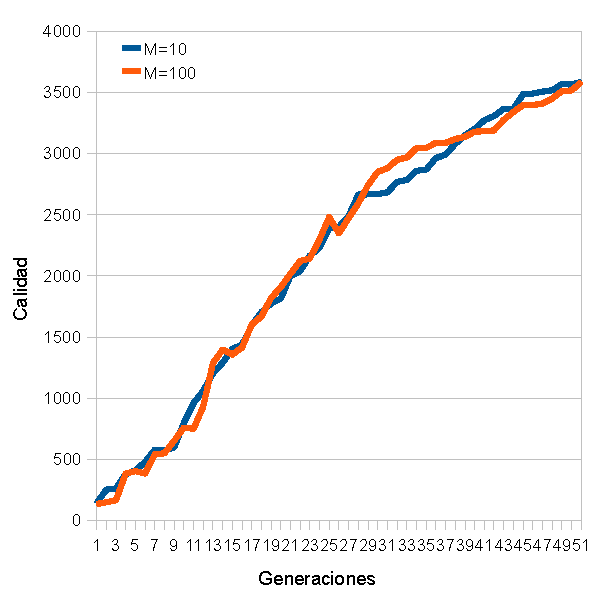
\includegraphics[width=0.4\textwidth]{figs/graphs/GrowMaxBest}
	\label{subfig:p-growdepth-best}
  }                
  \subfloat[Calidad media de la población]{
  	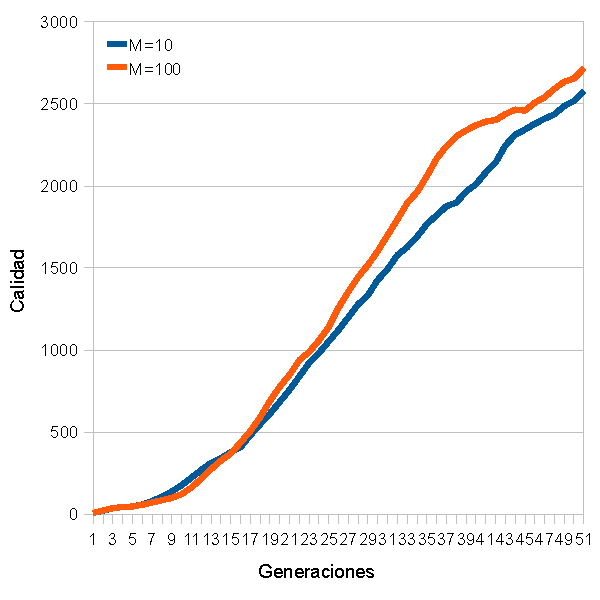
\includegraphics[width=0.4\textwidth]{figs/graphs/GrowMaxMean}
	\label{subfig:p-growdepth-mean}%
  }
  \quad
  \subfloat[Número de nodos medio de la población]{
  	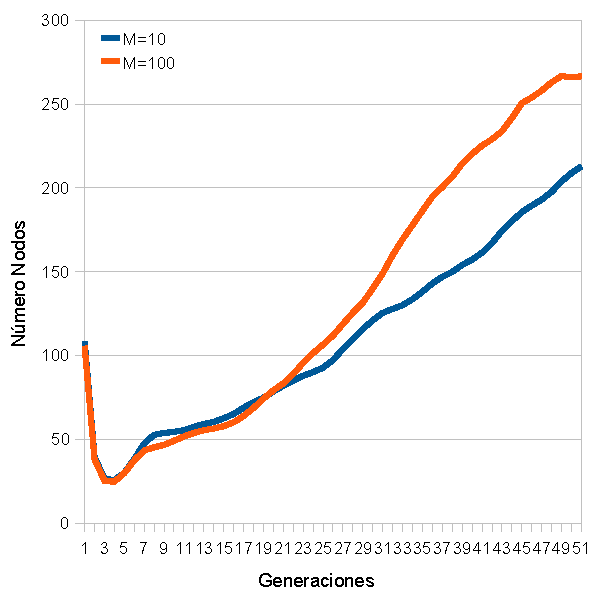
\includegraphics[width=0.4\textwidth]{figs/graphs/GrowMaxNodes}
	\label{subfig:p-growdepth-nodes}%
  }
  \subfloat[Tiempo de las ejecuciones]{
  	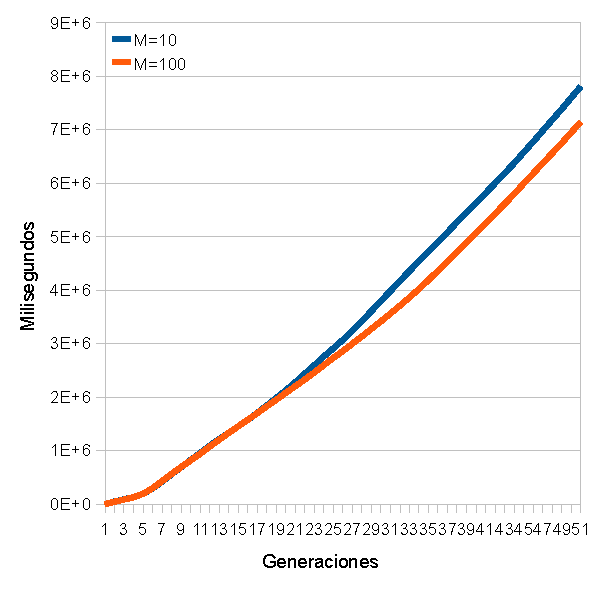
\includegraphics[width=0.4\textwidth]{figs/graphs/GrowMaxTime}
	\label{subfig:p-growdepth-time}%
  }
  \centering
\caption{Profundidad máxima del método grow ($M$)}
\label{fig:p-crosstries}
\end{figure}


\section{Profundidad máxima en el cruzamiento}\label{sec:p-prof-cross}

El parámetro de la profundidad máxima de cruzamiento se utilizará en el
cruzamiento de individuos e indica la profundidad máxima que tendrá el subárbol
seleccionado para ser intercambiado.

\begin{table}[tb]
\caption{Valores de los parámetros para la profundidad máxima en el
cruzamiento.}
\label{tab:prof-cross}
\centering
\begin{tabular}{lcc}
\toprule
  &\textbf{Prueba 13} & \textbf{Prueba 14}\\
\midrule
gp.koza.xover.maxdepth $30$ & $100$  \\
\bottomrule
\end{tabular}
\end{table}


Como indica claramente la figura \ref{subfig:p-maxdepthcross-best} y
\ref{subfig:p-maxdepthcross-mean} en el desempeño de los datos de la tabla
\ref{tab:prof-cross}, el mejor rendimiento se obtiene cuando la profundidad
máxima es menor, en concreto 17. Además se puede observar que el número de nodos
(figura \ref{subfig:p-maxdepthcross-nodes}) es mayor a lo largo del tiempo cuando
la profundidad máxima es mayor. Esto es debido cuanta más profundidad, mayor es
el número de nodos que intercambiamos. El rendimiento (figura
\ref{subfig:p-maxdepthcross-time}) muestra, fuera de lo esperado, una relación
indirectamente proporcional entre el tiempo y el número de nodos. Este evento
puede ser debido a que ambas pruebas albergan un número de nodos parecidos y
por ello, el rendimiento del arbol no depende únicamente del árbol de programa,
sino que influye la rapidez en la que se evaluan las condiciones del árbol. 


\begin{figure}[tb]
  \centering
  \subfloat[Calidad de los mejores individuos]{
  	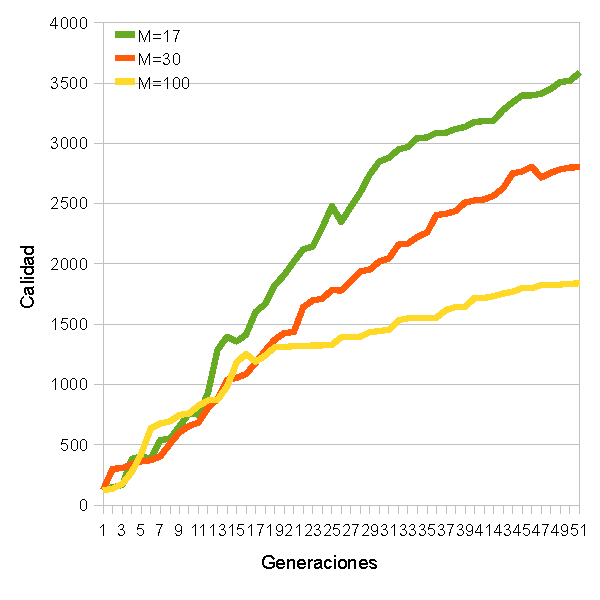
\includegraphics[width=0.4\textwidth]{figs/graphs/MaxDepthCrossBest}
	\label{subfig:p-maxdepthcross-best}
  }                
  \subfloat[Calidad media de la población]{
  	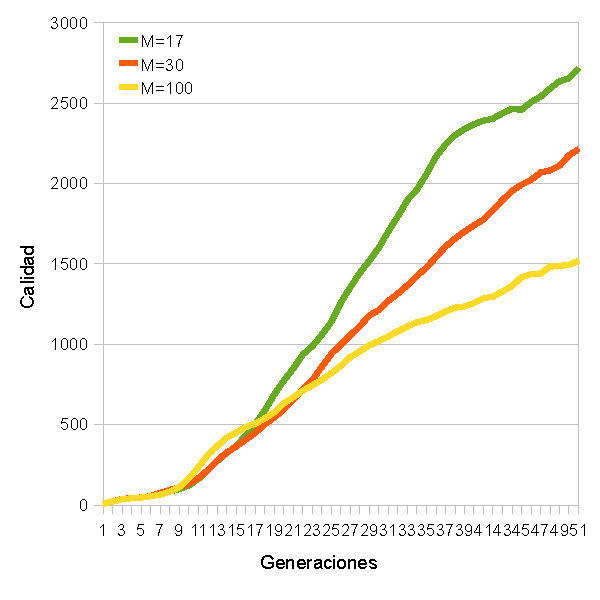
\includegraphics[width=0.4\textwidth]{figs/graphs/MaxDepthCrossMean}
	\label{subfig:p-maxdepthcross-mean}%
  }
  \quad
  \subfloat[Número de nodos medio de la población]{
  	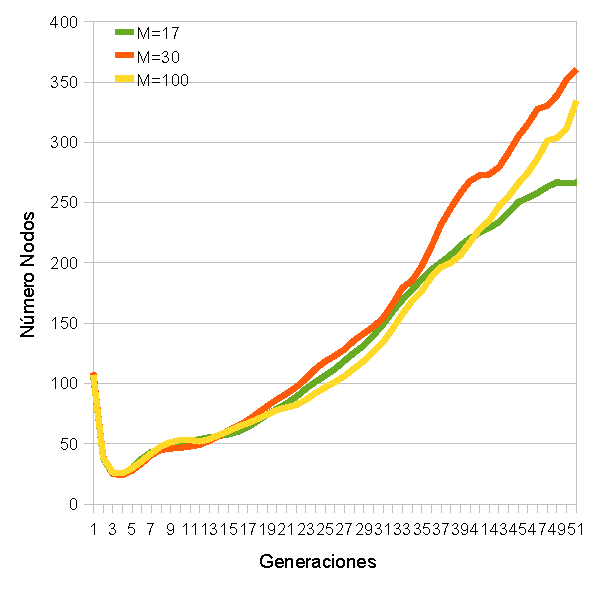
\includegraphics[width=0.4\textwidth]{figs/graphs/MaxDepthCrossNodes}
	\label{subfig:p-maxdepthcross-nodes}%
  }
  \subfloat[Tiempo de las ejecuciones]{
  	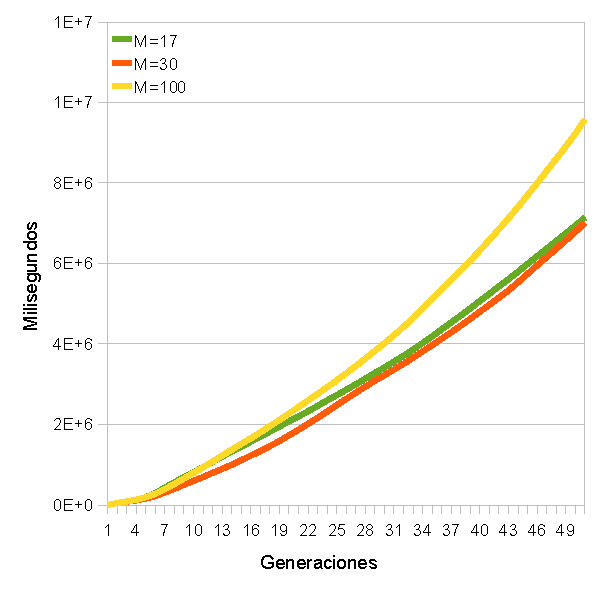
\includegraphics[width=0.4\textwidth]{figs/graphs/MaxDepthCrossTime}
	\label{subfig:p-maxdepthcross-time}%
  }
  \centering
\caption{Profundidad máxima en el cruzamiento ($M$)}
\label{fig:p-crosstries}
\end{figure}


\section{Profundidad máxima en la mutación}\label{sec:p-prof-mut}	

La profundidad máxima de mutación ajusta la longitud máxima que un subárbol
generado aleatoriamente podrá tener. Si el árbol excede esta profundidad, el
subárbol será descartado y se generará otro nuevo subárbol.

El comportamiento esperado es que según se aumenta la profundidad máxima, es más
probable que se generen árboles válidos, y, además, estos tendrán una longitud
mayor. En el caso que se disminuya la profundidad máxima, la mutación se
producirá con menos probabilidad y, en el caso de que aparezca el fenómeno, el
subárbol generado será de menor longitud.

\begin{table}[cbt]
\caption{Valores de los parámetros para la profundidad máxima en la mutación.}
\label{tab:prof-mut}
\centering
\begin{tabular}{lcc}
\toprule
  &\textbf{Prueba 15} & \textbf{Prueba 16}\\
\midrule
gp.koza.mutate.maxdepth & $30$ & $100$  \\
\bottomrule
\end{tabular}
\end{table}

Si observamos las gráficas de calidad (figura \ref{subfig:p-maxdepthmutate-best}
y \ref{subfig:p-maxdepthmutate-mean}) obtenidas mediante los parámetros de la
tabla \ref{tab:prof-mut}, observamos un fenómeno curioso. El mejor rendimiento
del algoritmo se encuentra cuando la profundad máxima es 17 y 100, sin embargo,
el peor desempeño lo tiene la ejecución con valor 30. La figura de número de
nodo \ref{subfig:p-mutatetries-nodes} y la figura del rendimiento
\ref{subfig:p-mutatetries-time} no indican ningún dato que resaltar.

Como el valor que mejor calidad ofrece es 100, optaremos por este valor de
configuración.


\begin{figure}[tb]
  \centering
  \subfloat[Calidad de los mejores individuos]{
  	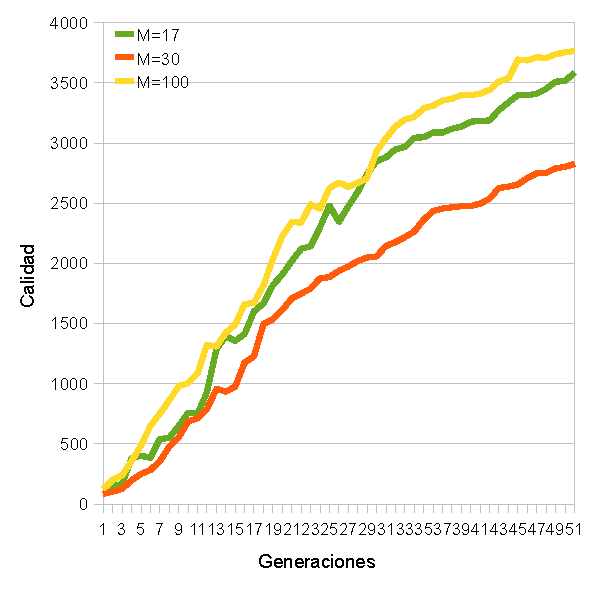
\includegraphics[width=0.4\textwidth]{figs/graphs/MaxDepthMutateBest}
	\label{subfig:p-maxdepthmutate-best}
  }                
  \subfloat[Calidad media de la población]{
  	\includegraphics[width=0.4\textwidth]{figs/graphs/MaxDepthMutateMean}
	\label{subfig:p-maxdepthmutate-mean}%
  }
  \quad
  \subfloat[Número de nodos medio de la población]{
  	\includegraphics[width=0.4\textwidth]{figs/graphs/MaxDepthMutateNodes}
	\label{subfig:p-maxdepthmutate-nodes}%
  }
  \subfloat[Tiempo de las ejecuciones]{
  	\includegraphics[width=0.4\textwidth]{figs/graphs/MaxDepthMutateTime}
	\label{subfig:p-maxdepthmutate-time}%
  }
  \centering
\caption{Profundidad máxima en la mutación ($M$)}
\label{fig:p-crosstries}
\end{figure}

\section{Factor fitness}\label{sec:p-factor-fitness}	

El factor del fitness es un valor que nos sirve para ponderar la suma de los
cubos resueltos de diferentes dificultades. De esta forma obtenemos una nota que
nos indica la calidad del individuo. La fórmula esta descrita en la sección
\ref{subsec:cubosresueltos}.

Un valor bajo, como 1, valora de la misma forma un cubo resuelto de nivel 1 que
de máximo, de tal forma que 10 cubos fáciles resueltos valen la misma puntuación
que 10 cubos difíciles resueltos. El único objetivo del algoritmo es resolver el
máximo número de cubos posibles independientemente de su dificultad.

Un valor más alto a 1, guía al proceso evolutivo a intentar resolver cubos de
mayor de dificultad ignorando los de menor dificultad. Así si el factor es 2, y
se resuelve un cubo de nivel 2, tendremos una puntuación de 4, y si otro
individuo resuelve 3 cubos de nivel uno, vencerá al individuo que resolvía uno de
nivel 2. De esta forma, cuanto más alto sea el valor del factor, mayor es la
importancia que tiene resolver un cubo de mayor dificultad.

Como el valor del fitness no es equiparable en cada prueba, compararemos las
pruebas con el valor medio de la entropía de cubos resueltos. De esta forma
podremos equiparar el desempeño de cada prueba.

\begin{table}[tb]
\caption{Valores de los parámetros para el factor del fitness.}
\label{tab:factor-fitness}
\centering
\begin{tabular}{lccc}
\toprule
  &\textbf{Prueba 17} & \textbf{Prueba 18} & \textbf{Prueba 19}\\
\midrule
gp.koza.fitness.factorfitness & $1$ & $2$ & $4$   \\
\bottomrule
\end{tabular}
\end{table}

En contra de lo que pensábamos, el resultado de las pruebas (figura
\ref{fig:p-factorfitness}) de los datos expuestos en la tabla
\ref{tab:factor-fitness} nos indica que el mejor rendimiento se obtiene cuando el
valor del factor es 1. Esto puede ser debido a que el sistema aprende a resolver
los casos básicos y lentamente va resolviendo casos más complicados.

\begin{figure}[tb]
  \centering
  \subfloat[Calidad de los mejores individuos]{
  	\includegraphics[width=0.4\textwidth]{figs/graphs/FactorFitnessBest}
	\label{subfig:p-factorfitness-best}
  }                
  \subfloat[Calidad media de la población]{
  	\includegraphics[width=0.4\textwidth]{figs/graphs/FactorFitnessMean}
	\label{subfig:p-factorfitness-mean}%
  }
  \quad
  \subfloat[Número de nodos medio de la población]{
  	\includegraphics[width=0.4\textwidth]{figs/graphs/FactorFitnessNodes}
	\label{subfig:p-factorfitness-nodes}%
  }
  \subfloat[Tiempo de las ejecuciones]{
  	\includegraphics[width=0.4\textwidth]{figs/graphs/FactorFitnessTime}
	\label{subfig:p-factorfitness-time}%
  }
  \centering
\caption{Factor fitness ($F$)}
\label{fig:p-factorfitness}
\end{figure}


\chapter{Participando en GECCO 2009}\label{ch:gecco2009}

The Genetic and Evolutionary Computation Conference (GECCO) es una de las 11
conferencias internacionales más importantes de inteligencia
artificial. En la conferencia se presentan los últimos resultados en el campo
en crecimiento de la computación evolutiva. Además se suelen hacer
competiciones donde la gente expone sus soluciones a los problemas dados.

Parabon es una empresa que se dedica a la computación distribuida a través de
su plataforma Frontier. Con animo de promocionar su plataforma, Parabon
patrocina una competición del GECCO 2009. Se trata de evolucionar un programa
que consiga resolver cualquier cubo de Rubik en el menor número de pasos
posibles.

La competición de Parabon exigía en sus bases que el programa se evolucionase
en su plataforma Frontier. Además Parabon ofrece otra plataforma para
desarrollar programación genética llamado Origin. Origin esta basado en ECJ,
una plataforma de computación evolutiva, adaptando ECJ para funcionar sobre
Frontier.

Al intentar utilizar Origin descubrimos que la plataforma estaba en vias de
desarrollo y resultaba casi imposible trabajar con ella. Es por esto que
migramos nuestro desarrollo a ECJ.

A partir de las experiencias anteriores se diseñó un experimento que tenía como
objetivo la generación de un programa capaz de tomar parte en la competición.

La simulación se llevó a cabo con los parámetros anteriormente determinados como
óptimos y con cubos de un máximo de 10 movimientos de desorden y con una cantidad
total de 2000 cubos diferentes aproximadamente. Este límite se debe a las
limitaciones del hardware en que tuvo lugar la misma.

La ejecución de la simulación se extendió durante 15 días y los resultados de la
misma fueron enviados a la competición. A pesar de que la competición fue
suspendida por falta de participantes válidos, la solución aportada fue
reconocida por los organizadores como la mejor participación. Los resultados de
la misma se resumen en la tabla \ref{tab:bestsolver}. Así mismo el programa
enviado se muestra en el apéndice \ref{sec:mejor-individuo}.


\begin{table}[tb]
\caption{Resultados de funcionamiento del mejor individuo.}
\label{tab:bestsolver}
\centering
\begin{tabular}{lccr}
\toprule
 \textbf{Dificultad} & \textbf{Resueltos} & \textbf{Total}&
  \textbf{Porcentaje}\\
\midrule
1 & 12 & 12 & 100.00\% \\
2&135&144&93.75\%\\
3&589&860&68.49\%\\
4&373&1000&37.30\%\\
5&148&1000&14.80\%\\
6&37&1000&3.70\%\\
7&12&1000&1.20\%\\
8&1&1000&0.10\%\\
9&2&1000&0.20\%\\
10&1&1000&0.10\%\\
\bottomrule
\textbf{Total}&1310&8016&16.34\%\\
\bottomrule
\end{tabular}
\end{table}




\chapter{Conclusiones}\label{ch:concl}

En el presente trabajo hemos abordado el problema de la generación automática,
mediante programación genética, de programas capaces de resolver cubos de Rubik.
Con este fin hemos definido un lenguaje apropiado para representar la solución
del problemay formulado una función de fitness adecuada para que nuestro sistema
evolutivo consiga desarrollarse y generar buenas soluciones. También hemos
propuesto un algoritmo de evaluación que obtenga datos suficientes para
determinar el rendimiento de programa que se está evolucionando.

Sobre la base de estas propuestas hemos realizado un estudio de los parámetros
del algoritmo evolutivo a la vez que se realizaron varias optimizaciones del
código usado.

En estos experimentos se logró tener soluciones capaces de resolver algunos cubos
de alto grado de desorden, en particular cubos que necesitaban hasta 10
movimientos para ser resueltos. Debido a las restricciones en cuanto a recursos
computacionales y tiempo dedicados a este trabajo fue imposible continuar
llevando a cabo estos experimentos. Hay que hacer notar que en un principio se
contaba con poder usar la plataforma de computación distribuida creada por
Parabon pero que esto no fue posible y solo se tuvo a disposición recursos
locales de cómputo.

A partir de las experiencias obtenidas en el estudio mencionado se evolucionó un
programa que fue enviado a la \textit{Parabon Sponsored GECCO Competition}.

A pesar de los inconvenientes prácticos que han impedido el completo despliegue
de la propuesta planteada se han obtenido varios resultados de interés. En
particular, se ha logrado una mejor comprensión de las características del
problema y se han identificado posibles líneas de solución.

Este trabajo puede ser mejorado de varios puntos de vista. Resulta de interés
comprobar las consecuencias de introducir elementos de optimización
multiobjectivo para así lograr una mejor representación del fitness.

Otro aspecto interesante sería introducir el concepto de subpoblaciones en el
proyecto. De esta forma, existirían varias poblaciones coexistiendo y
evolucionando paralelamente. En determinados momentos, estas subpoblaciones pueden
intercambiarse un número determinado de individuos. De esta forma, se aportaría
una nueva fuente de diversidad en las poblaciones.

También resulta importante encontrar un contexto adecuado para la ejecución de
los experimentos, ya sea en la plataforma de Parabon u otro ordenador o grupo de
ordenadores de alto desempeño.

Aunque no se haya conseguido crear un resolvedor universal de cubos de Rubik,
hemos asentado una base y unas lineas futuras de investigación con las que
esperamos que algún día el problema sea resuelto venciendo a los resolvedores
actuales creados mediante métodos de busqueda de todo el espacio de soluciones.

\backmatter


% para citar todo el .bib eliminar en tu version final
%\nocite{*}
\small
\bibliographystyle{apa-good}
\bibliography{bib/biblio}

\appendix
\chapter{Anexo}\label{ch:anexos}

\section{Gestión del proyecto}\label{sec:gestion-pr}

\includepdf[pages={1,2},landscape]{figs/planning.pdf}

\section{Parámetros de ECJ}\label{sec:ecj-params}

Fichero ec.params:

\begin{itemize}
\item verbosity = 0 : Es el nivel de mensajes que el sistema sacará por pantalla. Un número alto imprimirá más mensajes por pantalla.
\item	evalthreads=1 : Número de threads en el proceso de evaluación.
\item	breedthreads=1 : Número de threads en el proceso de reproducción.
\item	checkpoint=false : Activa o desactiva la opción de guardar el estado de
la evolución en una generación concreta.
\item	checkpoint-modulo = 1: Cada cuantas generaciones se haría el checkpoint.
\item	prefix = ec : Es el prefijo del nombre del fichero de checkpoint. 
\end{itemize}

El siguiente fichero en la jerarquía es simple.params. 

\begin{itemize}
\item	state = ec.simple.SimpleEvolutionState : esta clase define un modelo evolutivo generacional, es decir, cada generación es una nueva generación. Además se almacena la población de cada generación. Para poblaciones muy grandes y largas ejecuciones es mejor utilizar la clase  ec.steadystate.SteadyStateEvolutionState que mantiene una población, donde sus miembros van siendo reemplazados por los nuevos.
\item	init = 	ec.simple.SimpleInitializer : es la clase que se utilizará para inicializar la población.
\item	finish = ec.simple.SimpleFinisher :  es la clase que usa para finalizar
la población. Esta clase no hace nada actualmente.
\item	exch = ec.simple.SimpleExchanger : esta clase sirve para definir la forma
de intercambiarse individuos entre dos poblaciones. Esta clase tampoco hace nada.
\item	breed = ec.simple.SimpleBreeder : es la clase que asienta las bases de la reproducción. Se encargará de hacer el elitismo si se requiere. Sin embargo, esta clase solo escoge individuos dentro de la misma población.
\item	eval =	ec.simple.SimpleEvaluator :  es la clase que se encarga de administrar el procesos de evaluación de la población.
\item	stat =	ec.simple.SimpleStatistics : realiza estadísticas simples de la población.
\item	generations = 51 : número máximo de generaciones que podrán ejecutarse.
\item	quit-on-run-complete = true : activamos la opción de que el sistema pare cuando encontremos la mejor solución.
\item	pop = 	ec.Population : la clase de población que utilizaremos.
\item	pop.subpops = 1 : el número de subpoblaciones que tendremos
\item	pop.subpop.0 = ec.Subpopulation : la clase de subpoblación que existirá.
\item	pop.subpop.0.size =	1024 : el tamaño de la subpoblación 0
\item	pop.subpop.0.duplicate-retries = 0 : intentos de la subpoblación de eliminar los individuos repetidos de la población inicial 0.
\item	breed.elite.0 = 10 : espacio que dedicará para almacenar la élite de la población.
\item	stat.file \$out.stat : el nombre del fichero de estadísticas.
\end{itemize}

El próximo fichero en la jerarquía es koza.params:

\begin{itemize}
\item	pop.subpop.0.species.fitness = ec.gp.koza.KozaFitness : utilizaremos el fitness de koza.
\item	init = ec.gp.GPInitializer : Para inicializar la población se usará el inicializador de programación genética (GP).
\item	stat = ec.gp.koza.KozaStatistics : estadísticas de koza.
\item	pop.subpop.0.species = ec.gp.GPSpecies : especies de programación genética
\item	pop.subpop.0.species.ind = ec.gp.GPIndividual : individuos de programación genética.
\item	pop.subpop.0.duplicate-retries = 100 : se intentará 100 veces borrar a los individuos duplicados en la generación 0.
\item	pop.subpop.0.species.ind.numtrees = 1 : cada individuo tendrá un árbol.
\item	pop.subpop.0.species.ind.tree.0 = ec.gp.GPTree : este árbol será del tipo GPTree
\item	pop.subpop.0.species.ind.tree.0.tc = tc0 : Además tendrá la gramática tc0 (tree constrains).
\item	pop.subpop.0.species.pipe = ec.breed.MultiBreedingPipeline : lo individuos se someterán en la reproducción a varios sistemas de reproducción.
\item	pop.subpop.0.species.pipe.generate-max = false : no se intentará generar el máximo número de hijos.
\item	pop.subpop.0.species.pipe.num-sources = 2 : Se utilizarán dos formas de reproducción.
\item	pop.subpop.0.species.pipe.source.0 = ec.gp.koza.CrossoverPipeline : la primera será crossover.
\item	pop.subpop.0.species.pipe.source.0.prob = 0.9 : Se escogerá con una probabilidad de 0.9.
\item	pop.subpop.0.species.pipe.source.1 = ec.breed.ReproductionPipeline : en la segunda se utilizará la clonación.
\item	pop.subpop.0.species.pipe.source.1.prob = 0.1: con probabilidad 0.1.
\item	breed.reproduce.source.0 = ec.select.TournamentSelection : para seleccionar a los candidatos de la clonación se utilizará la selección por torneo(antes explicada).
\item	gp.koza.xover.source.0 = ec.select.TournamentSelection : para el proceso de crossover, el padre se buscará por el método de selección por torneo.
\item	gp.koza.xover.source.1 = same : la madre por el mismo sistema.
\item	gp.koza.xover.ns.0 = ec.gp.koza.KozaNodeSelector : para seleccionar el nodo en el padre que se cambiará, se utilizará el sistema de koza.
\item	gp.koza.xover.ns.1 = same : para la madre se utilizará el mismo sistema.
\item	gp.koza.xover.maxdepth = 17 : la máxima profundidad de los subárboles a escoger para el crossover será de 17 alturas.
\item	gp.koza.xover.tries = 1 : las veces que se intentará encontrar nodos compatibles para la reproducción.
\item	gp.koza.mutate.source.0 = ec.select.TournamentSelection : para mutar, se seleccionará a los individuos por torneo.
\item	gp.koza.mutate.ns.0 = ec.gp.koza.KozaNodeSelector : la selección del nodo a mutar se realizada por el método de Koza (aleatorio).
\item	gp.koza.mutate.build.0 = ec.gp.koza.GrowBuilder : Una vez que se localice el nodo, se reconstruirá el árbol por el método grow.
\item	gp.koza.mutate.maxdepth = 17 : es la profundidad máxima del subárbol a escoger. 
\item	gp.koza.mutate.tries = 1 : las veces que se intentará realizar la mutación con éxito.
\item	select.tournament.size = 7 : el número de individuos que entran en torneo.
\item	gp.koza.grow.min-depth = 5 : número de nodos mínimo de árbol del método grow.
\item	gp.koza.grow.max-depth = 5 : número máximo de nodos del método grow.
\item	gp.koza.ns.terminals = 0.1 : parámetro del selector de nodos, el cual seleccionará con probabilidad 0.1 terminales.
\item	gp.koza.ns.nonterminals = 0.9 : parámetro del selector de nodos, el cual seleccionará con probabilidad 0.9 noterminales.
\item	gp.fs.size = 1 : las siglas fs se refieren a Function Set. Sólo vamos a tener un grupo de funciones.
\item	gp.fs.0 = ec.gp.GPFunctionSet : nuestro grupo de funciones será del tipo GPFunctionSet.
\item	gp.fs.0.name = f0 : el nombre del grupo de función será f0.
\item	gp.type.a.size = 1 : tendremos solamente un tipo básico. Estos tipos básicos sirven para crear gramáticas y especifican el tipo de devuelta de los nodos.
\item	gp.type.a.0.name = nil : el nombre de este tipo básico es nil.
\item	gp.type.s.size = 0 : no tendremos ningún tipo compuesto.
\item	gp.tc.size = 1 : el tamaño de restricciones del árbol es de 1.
\item	gp.tc.0 = ec.gp.GPTreeConstraints : la clase para controlar estas restricciones es GPTreeConstraints.
\item	gp.tc.0.name = tc0 : el nombre de la restricciones sintácticas del árbol. Este debe coincidir con el especificado en el parámetro pop.subpop.0.species.ind.tree.0.tc.
\item	gp.tc.0.fset = f0 : el nombre del grupo de funciones.
\item	gp.tc.0.returns = nil : el tipo de devuelta del nodo base del árbol.
\item	gp.tc.0.init = ec.gp.koza.HalfBuilder : Es el constructor inicial del árbol. Mezcla el método grow y el método full.
\item	gp.koza.half.min-depth = 2 : es la mínima profundidad de los árboles generados.
\item	gp.koza.half.max-depth = 6 : es la profundidad máxima del árbol.
\item	gp.koza.half.growp = 0.5 : es la probabilidad que utilizará el método grow frente al método full.
\item	gp.nc.size = 7 : es el  número de restricciones sintácticas.
\item	gp.nc.0 = ec.gp.GPNodeConstraints : la clase que soporta estas restricciones.
\item	gp.nc.0.name = nc0 : el nombre de esta restricción.
\item	gp.nc.0.returns = nil : el tipo de devuelta esta restricción.
\item	gp.nc.0.size = 0 : el número de hijos que tendrá el nodo al que se aplique esta restricción. 
\item	gp.nc.1.child.0 = nil : cuando el número de hijos es mayor que cero hay que especificar el tipo de hijo que se requiere.
\end{itemize}

\section{Mejor Individuo}\label{sec:mejor-individuo}

(Progn2 (If (No (And (Test X1 Y1 FaceRight Color2) (Test X1 Y2 FaceBack Color1)))
(Move FaceDown Clockwise)) (Progn2 (If (No (And (Test X1 Y2 FaceUp Color1) (Test
X1 Y1 FaceFront Color5))) (Move FaceUp CounterClockwise)) (If (Or (Or (No (Test
X0 Y2 FaceUp Color1)) (Or (No (Test X0 Y2 FaceUp Color1)) (And (Test X1 Y1
FaceFront Color5) (And (No (And (Test X1 Y2 FaceUp Color1) (Test X1 Y1 FaceFront
Color5))) (Test X2 Y2 FaceFront Color1))))) (Or (Or (No (Test X0 Y2 FaceUp
Color1)) (And (And (And (Or (Or (No (Test X0 Y2 FaceUp Color1)) (Or (No (Test X0
Y1 FaceDown Color2)) (Test X0 Y2 FaceUp Color1))) (No (Or (Test X1 Y2 FaceUp
Color1) (Test X1 Y1 FaceDown Color2)))) (And (And (Test X1 Y1 FaceUp Color1)
(Test X1 Y1 FaceFront Color5)) (Or (No (Test X0 Y2 FaceUp Color1)) (And (And (And
(Test X1 Y1 FaceDown Color2) (Test X0 Y1 FaceDown Color2)) (Test X1 Y2 FaceUp
Color1)) (No (And (Test X1 Y1 FaceRight Color2) (Test X1 Y2 FaceBack
Color1))))))) (Test X1 Y2 FaceBack Color1)) (No (Test X2 Y2 FaceDown Color3))))
(No (Or (Or (Or (Or (Test X1 Y2 FaceUp Color1) (No (Test X1 Y2 FaceLeft Color0)))
(Test X1 Y1 FaceDown Color2)) (Test X1 Y2 FaceBack Color1)) (Test X1 Y1 FaceDown
Color2))))) (Move FaceLeft CounterClockwise))))

%\printindex
%\printindex[autx]
\end{document}
